% This is a template for Ph.D. dissertations in the UCI format.

% All fonts, including those for sub- and superscripts, must be 10 points or larger.
% Recommended sizes are 14-point for chapter headings, 12-point for the main body of text
% and figure/table titles, and 10-point for footnotes, sub- and super-scripts, and text in
% figures and tables.
\documentclass[12pt,fleqn]{ucithesis}

\usepackage{amsmath}
\usepackage{amsthm}
\usepackage{alltt}
\usepackage{paralist}
\usepackage{listings}
\usepackage{times}
\usepackage{clrscode}
\usepackage{ccaption}
\usepackage{array}
\usepackage{bm}
\usepackage{boxedminipage}
\usepackage{graphicx}
\usepackage{natbib}
\usepackage{path}
\usepackage{psfrag}
\usepackage{relsize}
\usepackage{mdwtab}
\usepackage{subfigure}
%\usepackage[ruled]{algorithm2e}
\usepackage{epsfig}
\usepackage{multirow}
\usepackage{float}
\usepackage{graphics}
\usepackage{epstopdf}
\usepackage{url}

\usepackage{xr}
\usepackage{courier}

\usepackage{alltt}
\usepackage{graphicx}
\usepackage{color}



% plainpages=false fixes the "duplicate ignored" error with page counters
% Set pdfborder to 0 0 0 to disable colored borders around PDF hyperlinks
% Use linktocpage=true to avoid figure captions not being split properly.
\usepackage[plainpages=false,pdfborder={0 0 0},linktocpage=true]{hyperref}
\usepackage{breakurl}

% Uncomment the following line to enable Unicode support. This will allow you
% to enter non-ASCII characters (such as accented characters) directly without
% having to use LaTeX's awkward escape syntax (e.g., \'{e})
% NOTE: You may have to install the ucs.sty package for this to work. See:
% http://www.unruh.de/DniQ/latex/unicode/
% \usepackage[utf8x]{inputenc}

\setcounter{secnumdepth}{3}
%\setcounter{tocdepth}{3}

\newcommand{\ttfont}[1]{\ensuremath{\tt{#1}}}
\newcommand{\ed}{\ensuremath{\sf{ed}}}

\newcommand{\thickhline}{\noalign{\hrule height 0.8pt}}

\newcommand{\eat}[1]{}
\newcommand{\codepiece}[1]{\texttt{\small #1}}
%% Prelim chapter
\usepackage{listings}

\urlstyle{same}

% configuration for listings
\definecolor{light-gray}{gray}{0.98}
\definecolor{dark-gray}{gray}{0.5}
\lstset{frame=single, backgroundcolor=\color{light-gray}, basicstyle=\ttfamily\scriptsize
}
\lstMakeShortInline^

\def\aroundlstskip{0ex}
\lstdefinestyle{noskip}{aboveskip=\aroundlstskip,belowskip=\aroundlstskip,abovecaptionskip=\aroundlstskip,belowcaptionskip=\aroundlstskip}
\lstnewenvironment{code}{}{}

\newcommand{\citeurl}[1]{{\scriptsize \textsf{#1}}}

\lstdefinelanguage{AQL}{
  alsoletter={-"'_:\$[]()0123456789\\},
  morekeywords={
    for,
    let,
    in,
    return,
    where,
    group,
    by,
    with,
    order,
    desc,
    asc,
    limit,
    replace,
    delete,
    insert,
    into,
    some,
    every,
    satisfies,
    and,
    or,
    use,
    dataverse,
    set,
    simfunction,
    simthreshold,
    create,
    index,
    type,
    fuzzy,
    keyword,
    NGram,
    rtree
  },
  basicstyle=\sf,
  keywordstyle=\textbf,
  identifierstyle=\texttt,
  commentstyle=\textit,
  literate={<=}{{\litleq}}1 {>=}{{\litgeq}}1,
  literate={~=}{$\sim{}=$}1 % set tilde as a literal (no process)
}[keywords,comments,strings]

\lstdefinelanguage{AQLSchema}{
  alsoletter={-"'_:(\$\\},
  morekeywords={
    use,
    declare,
    type,
    as,
    open,
    closed,
    dataset,
    dataverse,
    nodegroup,
    on,
    partitioned,
    by,
    primary,
    key,
    create,
    index,
    int32,
    string,
    datetime,
    double,
    date,
    point,
    with,
    filter
  },
  basicstyle=\sf,
  keywordstyle=\textbf,
  identifierstyle=\texttt,
  commentstyle=\textit,
  literate={<=}{{\litleq}}1 {>=}{{\litgeq}}1
}[keywords,comments,strings]


\lstdefinelanguage{AQLSchema2}{
  alsoletter={-"'_:(\$\\},
  morekeywords={
    use,
    declare,
    type,
    as,
    open,
    closed,
    dataset,
    dataverse,
    nodegroup,
    on,
    partitioned,
    by,
    primary,
    key,
    create,
    index,
    int32,
    string,
    datetime,
    double,
    date,
    point,
    with,
    filter,
    TwitterUserType
  },
  basicstyle=\sf,
  keywordstyle=\textbf,
  identifierstyle=\texttt,
  commentstyle=\textit,
  literate={<=}{{\litleq}}1 {>=}{{\litgeq}}1
}[keywords,comments,strings]

\lstnewenvironment{aql}
   {\lstset{language=AQL,columns=space-flexible,basicstyle=\small,basewidth={.5em,.5em}}}
   {}

\lstnewenvironment{aqlscriptsize}
   {\lstset{language=AQL,columns=space-flexible,basicstyle=\scriptsize,basewidth={.5em,.5em},numbers=left}}
   {}

\lstnewenvironment{aqltiny}
   {\lstset{language=AQL,columns=space-flexible,basicstyle=\tiny,basewidth={.5em,.5em},numbers=left}}
   {}

\lstnewenvironment{aqlschema}
   {\lstset{language=AQLSchema,columns=space-flexible,basicstyle=\small,basewidth={.5em,.5em}}}
   {}
   
\lstnewenvironment{aqlschema2}
   {\lstset{language=AQLSchema2,columns=space-flexible,basicstyle=\small,basewidth={.5em,.5em}}}
   {}

\lstdefinelanguage{SQL}{%
  alsoletter={-_:(\$\\},
  morekeywords={
    select,
    from,
    where,
    and,
    or,
    in,
    as,
    group,
    by,
    join,
    on,
    with,
    update,
    set,
    delete,
    insert
  },
  basicstyle=\sf,
  keywordstyle=\textbf,
  identifierstyle=\texttt,
  commentstyle=\textit,
  literate={<=}{{\litleq}}1 {>=}{{\litgeq}}1 {//}{{\litdoubleslash}}1 %%{::}{{\litdoublecolon}}1%
}[keywords,comments,strings]


\lstnewenvironment{sql}
   {\lstset{language=SQL,columns=flexible,basicstyle=\footnotesize,basewidth={.3em,.2em}}}
   {}


\lstdefinelanguage{SQLSchema}{
  alsoletter={-"'_:(\$\\},
  morekeywords={
    CREATE,
    TABLE,
    INTEGER,
    CHAR,
    VARCHAR
  },
  basicstyle=\sf,
  keywordstyle=\textbf,
  identifierstyle=\texttt,
  commentstyle=\textit,
  literate={<=}{{\litleq}}1 {>=}{{\litgeq}}1
}[keywords,comments,strings]

\lstnewenvironment{sqlschema}
   {\lstset{language=SQLSchema,columns=flexible,basicstyle=\scriptsize,basewidth={.5em,.5em}}}
   {}

\lstdefinelanguage{Java}{
  alsoletter={-"'_},
  morekeywords={
    public,
    interface,
    for,
    while
    return.
    class
  },
  basicstyle=\sf,
  keywordstyle=\textbf,
  identifierstyle=\texttt,
  commentstyle=\textit,
}[keywords,comments,strings]

\lstnewenvironment{java}
   {\lstset{language=Java,columns=flexible,basicstyle=\scriptsize,tabsize=4,basewidth={.3em,.2em}}}
   {}


\newlength{\columnfigurewidth}
\setlength{\columnfigurewidth}{\columnwidth}

\newcounter{ddlcnt}
\lstnewenvironment{ddl}[2][]{
  \renewcommand{\lstlistingname}{Data definition}
  \setcounter{lstlisting}{\value{ddlcnt}}
  \lstset{style=noskip,captionpos=b,float=h!t,caption=#1,label=#2}
}{
  \addtocounter{ddlcnt}{1}
}

\newcounter{querycnt}
\lstnewenvironment{query}[2][]{
  \renewcommand{\lstlistingname}{Query}
  \setcounter{lstlisting}{\value{querycnt}}
  \lstset{style=noskip,captionpos=b,float=h!t,caption=#1,label=#2}
}{
  \addtocounter{querycnt}{1}
}

\newcounter{updatecnt}
\lstnewenvironment{update}[2][]{
  \renewcommand{\lstlistingname}{Update}
  \setcounter{lstlisting}{\value{updatecnt}}
  \lstset{style=noskip,captionpos=b,float=h!t,caption=#1,label=#2}
}{
  \addtocounter{updatecnt}{1}
}

\newcommand{\flwor}{\textsl{\textbackslash'fla$\dot{\mbox{u}}$(-\textreve)r\textbackslash}}

\newcommand{\TODO}[1] {\textbf{TODO \textsc{#1}}}

\renewcommand*{\thefootnote}{\fnsymbol{footnote}}




\begin{document}

\thesistitle {
An Efficient Foundation for Big Data Processing on Modern Clusters
}

\degreename{Doctor of Philosophy}

% Use the wording given in the official list of degrees awarded by UCI:
% http://www.rgs.uci.edu/grad/academic/degrees_offered.htm
\degreefield{Information and Computer Science}

% Your name as it appears on official UCI records.
\authorname{Vinayak Borkar}

% Use the full name of each committee member.
\committeechair{Professor Michael J. Carey}
\othercommitteemembers
{
Professor Chen Li \\
Professor Sharad Mehrotra \\
Professor Vassilis Tsotras
}

\degreeyear{2016}

\copyrightdeclaration
{
{\copyright} {\Degreeyear} \Authorname
}

% If you have previously published parts of your manuscript, you must list the
% copyright holders; see Section 3.2 of the UCI Thesis and Dissertation Manual.
% Otherwise, this section may be omitted.
\prepublishedcopyrightdeclaration
{
Portions of Chapter 3 {\copyright} 2011 IEEE \\
Portions of Chapter 4 {\copyright} 2015 ACM \\
Portions of Chapter 5 {\copyright} 2014 VLDB Endowment \\
All other materials {\copyright} 2016 \Authorname
}

% The dedication page is optional.
%\dedications {
%}

\acknowledgments {
This thesis would not have been possible but for the constant encouragement from my advisor, Dr. Michael J. Carey. It has been an ongoing effort from his side for the past twelve years to have me pursue a PhD. degree.

Since 2009, when I started working on Hyracks, I have had the opportunity to work with some of the smartest people, both in and out of academia, who have shaped the work I did as well as my approach to technical problems. During my tenure at UCI, I realized that building a robust system involving close to half a million lines of code is not an easy feat and would not have been possible without the conviction and sacrifices made by all involved. I would like to thank Dr. Michael Carey, Dr. Chen Li, and Dr. Vassilis Tsotras for being part of the AsterixDB effort, and allowing their students to spend an enormous amount of time to develop the AsterixDB codebase, even though that work would not directly translate to published papers.

I would like to thank Yingyi Bu, Preston Carman Jr., Raman Grover, Nicola Onose, Pouria Pirzadeh, Rares Vernica, and Till Westmann for being my co-conspirators in the Hyracks and Algebricks efforts.

AsterixDB has been the work of many people over the last several years. Sattam Alsubaiee, Alex Behm, Khurram Faraaz, Raman Grover, Zachary Heilbron, Young-Seok Kim, Nicola Onose, Rares Vernica, and Till Westmann were instrumental in building and maintaining large parts of the AsterixDB codebase. I have benefited from valuable discussions with them during my tenure at UCI.

I would like to specially thank Tyson Condie for building the Overlog platform that helped us to quickly prototype parts of Hyracks. Tyson was also instrumental in connecting us with Chris Jermaine and his students, who at that time were looking for a platform to experiment with online-aggregation. Hyracks turned out to be a good fit for that work. While at Yahoo Research, Tyson helped us to get access to a 180-node cluster to scale-test Hyracks.

The data team at Facebook was very generous in awarding me a Facebook Fellowship for my work on Hyracks and then providing me access to their Hive cluster. Working on their cluster gave me a lot of insight into some of the real challenges involved in running a Big Data environment. I am very grateful to them for this opportunity.

Last, but not least, I would like to thank my family for letting me pursue this work for such a long period of time, finally to its completion.
}

% Include, at minimum, a listing of your degrees and educational
% achievements with dates and the school where the degrees were
% earned. Also include the degree currently being attained.
\curriculumvitae
{
  % The following is a sample CV to get you started. Feel free to
  % change it however you wish; there are no specific requirements
  % regarding the formatting of your CV.

  \textbf{EDUCATION}

  \begin{tabular*}{1\textwidth}{@{\extracolsep{\fill}}lr}
    \textbf{Doctor of Philosophy in Information} & \textbf{2016} \\
    \textbf{and Computer Science} & \\
    \vspace{6pt}
    University of California, Irvine & \emph{Irvine, California} \\
    \textbf{Master of Technology in Computer Science} & \textbf{2001} \\
    \vspace{6pt}
    Indian Institute of Technology, Bombay & \emph{Mumbai, India} \\
    \textbf{Bachelor of Engineering in Computer Science} & \textbf{1999} \\
    \vspace{6pt}
    University of Mumbai & \emph{Mumbai, India} \\
  \end{tabular*}

  \vspace{12pt}
  \textbf{SELECTED HONORS AND AWARDS}

  \begin{tabular*}{1\textwidth}{@{\extracolsep{\fill}}lr}
    \textbf{Facebook Fellowship Award} & \textbf{2011} \\
    \textbf{Graduated First from the Computer Science Department at IIT, Bombay} & \textbf{2001} \\
    \textbf{Research Fellowship by IBM for excellent academic performance} & \textbf{2000-2001} \\
  \end{tabular*}

  \pagebreak

  \textbf{PUBLICATIONS}

  \begin{tabular*}{1\textwidth}{@{\extracolsep{\fill}}p{5in}r}
    \textbf{Algebricks: a data model-agnostic compiler backend for big data languages} & \textbf{2015} \\
    \multicolumn{2}{@{\extracolsep{\fill}}l}{Symposium on Cloud Computing} \vspace{6pt} \\

    \textbf{Storage Management in AsterixDB} & \textbf{2014} \\
    \multicolumn{2}{@{\extracolsep{\fill}}l}{International Conference on Very Large Databases (VLDB)} \vspace{6pt} \\

    \textbf{AsterixDB: A Scalable, Open Source BDMS} & \textbf{2014} \\
    \multicolumn{2}{@{\extracolsep{\fill}}l}{International Conference on Very Large Databases (VLDB)} \vspace{6pt} \\

    \textbf{Pregelix: Big(ger) Graph Analytics on a Dataflow Engine} & \textbf{2014} \\
    \multicolumn{2}{@{\extracolsep{\fill}}l}{International Conference on Very Large Databases (VLDB)} \vspace{6pt} \\

    \textbf{A Common Compiler Framework for Big Data Languages: Motivation, Opportunities, and Benefits} & \textbf{2013} \\
    \multicolumn{2}{@{\extracolsep{\fill}}l}{IEEE Data Engineering Bulletin 36(1)} \vspace{6pt} \\

    \textbf{Scuba: Diving into Data at Facebook} & \textbf{2013} \\
    \multicolumn{2}{@{\extracolsep{\fill}}l}{International Conference on Very Large Databases (VLDB)} \vspace{6pt} \\

    \textbf{A bloat-aware design for big data applications} & \textbf{2013} \\
    \multicolumn{2}{@{\extracolsep{\fill}}l}{International Symposium on Memory Management} \vspace{6pt} \\

    \textbf{Declarative Systems for Large-Scale Machine Learning} & \textbf{2012} \\
    \multicolumn{2}{@{\extracolsep{\fill}}l}{IEEE Data Engineering Bulletin 35(2)} \vspace{6pt} \\

    \textbf{ASTERIX: An Open Source System for ``Big Data'' Management and Analysis (Demo)} & \textbf{2012} \\
    \multicolumn{2}{@{\extracolsep{\fill}}l}{International Conference on Very Large Databases (VLDB)} \vspace{6pt} \\

    \textbf{ASTERIX: towards a scalable, semistructured data platform for evolving-world models} & \textbf{2011} \\
    \multicolumn{2}{@{\extracolsep{\fill}}l}{Distributed and Parallel Databases} \\

    \textbf{Online Aggregation for Large MapReduce Jobs} & \textbf{2011} \\
    \multicolumn{2}{@{\extracolsep{\fill}}l}{International Conference on Very Large Databases (VLDB)} \vspace{6pt} \\

    \textbf{Map-reduce extensions and recursive queries} & \textbf{2011} \\
    \multicolumn{2}{@{\extracolsep{\fill}}l}{International Conference on Extending Database Technology (EDBT)} \vspace{6pt} \\

    \textbf{Hyracks: A flexible and extensible foundation for data-intensive computing} & \textbf{2011} \\
    \multicolumn{2}{@{\extracolsep{\fill}}l}{International Conference on Data Engineering (ICDE)} \vspace{6pt}
  \end{tabular*}
}

%%% Local Variables: 
%%% mode: latex
%%% TeX-master: "thesis"
%%% End: 

\thesisabstract { 
In recent years, the world has seen an explosion in the amount of data being generated. Google proposed the MapReduce framework to allow programmers easily process massive amounts of data in parallel using a cluster of shared-nothing commodity machines. What started out as a tool for human efficiency subsequently began to be used as an intermediate representation for queries compiled from higher-level declarative languages. In this thesis, we present an alternate software stack for building scalable Big Data systems. We specifically focus on two parts of the stack. Hyracks is a new partitioned-parallel runtime layer that provides an efficient, generalized model for executing data-processing jobs on a cluster of commodity machines. Algebricks is a compiler framework that helps to build high-level declarative language compilers for parallel processing on top of Hyracks.
}


\preliminarypages

\chapter{Introduction}
\label{ch:intro}

In recent years, the world has seen an explosion in the amount of data. Initially, this data growth was triggered by the popularity of the Internet, but in the last few years, the growth of social networks such as Facebook, and micro-blogging services such as Twitter, have been responsible for producing ever-growing volumes of data. Over the same period of time, the declining cost of hardware has made it economically possible to set up sizable clusters of cheap computers to store and process this data. However, programming a cluster of shared-nothing computers is not an easy problem. Parallel programming has always been a hard problem, mostly owing to the lack of high-level abstractions to simplify the task.

Google, being at the forefront of this data-tsunami building a web-scale search engine, built the MapReduce \cite{mapreduce} programming model to enable their programmers to be productive on shared-nothing clusters. The MapReduce platform motivated the creation of the Hadoop \cite{hadoop:website}, an open source implementation of the MapReduce model. This development kick-started the new age of Big Data systems.

Initially, programmers used the MapReduce system to implement tools to quickly comb through very large amounts of data stored on clusters of commodity machines. Over time, it was clear that writing these tools in imperative languages, for analysis, was not the best use of programmers' time. To further improve programmer productivity, higher-level declarative languages were implemented (Sawzall~\cite{sawzall} and Tenzing~\cite{tenzing}, at Google, and Hive~\cite{hive}, at Facebook). The runtime layer used to process queries by these systems was still the MapReduce platform. While MapReduce was a simple model for programmers writing simple tools, we believed that it was the wrong layer for query language compilers to target, as their runtime layer. Sticking to the MapReduce abstraction forced queries to be evaluated as a sequence of MapReduce jobs with intermediate data materialized in a distributed filesystem, thus using a whole lot of unneeded resources. Several decades of database research has shown that pipelined architectures for executing queries consume fewer system resources, making better use of available hardware. One other problem with the MapReduce model was the reliance on unary operators for implementing Map and Reduce functions. This limitation of the model forces the need to express binary operations (such as joins) in an unnatural convoluted fashion. For example, Hive implements join over the MapReduce platform by expressing the operation as a grouping of the tagged union of the two relations being joined.
Another type of inefficiency introduced by the MapReduce platform has to do with the limited types of query processing algorithms that can be implemented within the framework, owing to the strict map-followed-by-sort-followed-by-reduce contract. For example, aggregation in MapReduce is implemented using a sort-based strategy because sorting is built into the system. A traditional parallel relational database system might have chosen a hash-based strategy to perform aggregation. This choice would require that the platform provide data redistribution primitives that offer more control. More details of these inefficiencies are described in Chapter~\ref{ch:hyracks}. Based on these observations, we designed and implemented Hyracks, a high-performance parallel dataflow runtime layer.

Hyracks was being built in the context of AsterixDB~\cite{ASTERIX}, a full-fledged, semi-structured, parallel big data management system that featured a fully functional declarative query language called AQL. As we started to build the query compilation layer for AQL, we realized that there was an opportunity to design the compilation framework in such a way that it could be re-purposed to build other declarative languages to be evaluated on the Hyracks platform. We called this layer Algebricks. Every query compiler built for parallel data-processing at the time (\cite{hive}, \cite{conf/sigmod/OlstonRSKT08}) was being built from scratch with its own parser, an intermediate representation based on an algebra, an optimizer to optimize queries, and finally a code generator to produce the runtime code. We designed Algebricks to provide an algebraic intermediate representation that was general enough to capture the semantics of the known languages, and also to be extensible to capture semantics of new, yet-to-come query languages of the future. Algebricks provides a rule-based optimizer and a library of generally applicable rewrite rules that can be used to quickly put together a compiler for a new declarative language. Algebricks also provides a code generator that compiles optimized queries to Hyracks jobs. Details of the Algebricks library can be found in Chapter~\ref{ch:algebricks}.

Figure~\ref{fig:asterixdb_stack} shows the various layers of the software stack that rests on the Hyracks platform. Algebricks, shown to the left of the figure, supports the AsterixDB compiler. In addition, we modified the Hive compiler to use Algebricks and run Hive queries as Hyracks jobs. Apache VXQuery~\cite{DBLP:conf/bigdataconf/CarmanWBCT15} is an open-source XQuery processor that has since been built to use Algebricks as its compilation framework to run queries over large amounts of XML data, on top of the Hyracks platform.

\begin{figure}[htb]
\centering
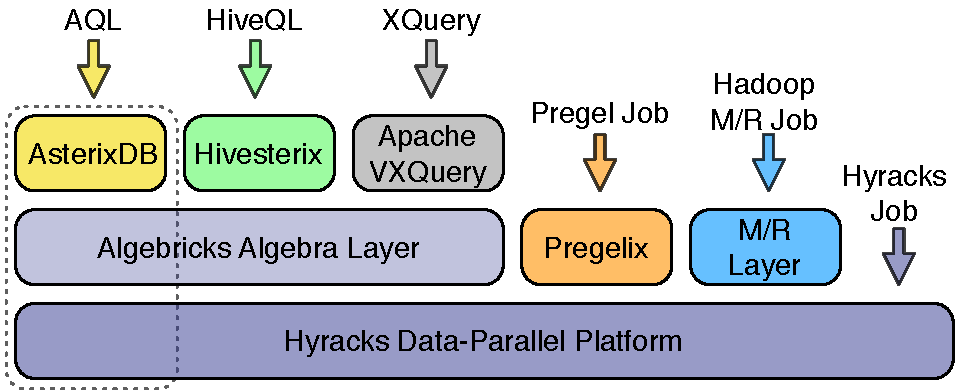
\includegraphics[width=6in]{images/asterixdb_stack}
%\vspace*{\betweenfigureandcaption}
\caption{Asterix software stack\label{fig:asterixdb_stack}}
%\vspace{-0.1in}
\end{figure}

Hyracks has also been successfully used to implement a clone of Pregel~\cite{Pregel}, called Pregelix~\cite{pregelix}. Pregelix implements a parallel framework to perform graph data processing at scale. Underneath, it uses Hyracks to implement the Pregel model using dataflow primitives. In terms of performance, it beats the foremost process-parallel open-source Pregel implementation called Giraph~\cite{giraph}. More details about the implementation of Pregelix are out of scope of this thesis, but can be found in \cite{pregelix}.

We proceed next to explore the related work in this area in Chapter~\ref{ch:foundations}. In Chapter~\ref{ch:hyracks} we describe the design and implementation of the Hyracks layer followed by that of Algebricks in Chapter~\ref{ch:algebricks}. Chapter~\ref{ch:asterixdb} describes how AsterixDB was built using Hyracks and Algebricks. Finally, we conclude in Chapter~\ref{ch:conclusions-and-future-work}.

\chapter{Related Work}
\label{ch:foundations}

In this chapter, we describe existing systems and research related to Big Data systems. Hyracks builds upon prior work in the area of Parallel Database systems and Data-Intensive computing. We start by providing a brief history of Parallel Database systems, followed by and overview of Data-Intensive computing systems.

\section{Parallel Database Systems}

The period from the early 80s to the mid-90s of the previous century saw a flurry of work in the area of parallel database systems, both in the research community as well as in industry. The Gamma Database Machine Project~\cite{GammaVLDB,GammaTKDE} was a parallel database research project that was developed at the University of Wisconsin, Madison. Gamma was based on a shared-nothing architecture consisting of a number of a number of processors connected to each other by a communication network. The shared-nothing architecture showed promise of being scalable to 1000s of nodes. Gamma applied partitioned-parallel techniques to process SQL queries over relational data. They used hash-based parallel algorithms owing to their theoretical infinite scalability due to the lack of a need for centralized control. Gamma's predecessor, DIRECT~\cite{DBLP:journals/tse/BoralDFJW82}, had shown that centralized control was an impediment to scalability.

Around the same timeframe as Gamma, the GRACE Database Machine project~\cite{GRACE} was being developed at the University of Tokyo, in Japan. The GRACE machine performed parallel query processing using a combination of hashing and sorting. The Grace hash join was a by-product of this project.

Teradata~\cite{Teradata} was an industrial parallel database, also based on the shared-nothing architecture, that used principles similar to Gamma and the GRACE projects. In the early 90s, Teradata was already shipping parallel database systems that scaled to around 200 processors.

In \cite{DewittGrayPDB}, DeWitt and Gray provide an excellent summary of parallelization techniques that have been successfully used by parallel database systems to achieve very high scalability.

\section{Data-Intensive Computing Systems}

The area of data-intensive computing was kick-started by the introduction of the MapReduce~\cite{mapreduce} system by Google. MapReduce provided a simple programming abstraction for developers to build data-processing tools that could process massive quantities of data distributed across thousands of machines. The MapReduce platform assumes that data is organized as files that are split into blocks and stored in a distributed filesystem (such as the Google Filesystem~\cite{GFS-Paper}). The MapReduce model allows programmers to express data processing tasks by implementing a combination of Map and Reduce functions. The infrastructure then applies these functions in parallel to large quantities of data to achieve the final result. For example, if one was interested in counting the number of unique words in a large number of text files, they would write a Map function that scanned through the lines of the text file to tokenize each line into words and produce (<word>, 1) pairs. The MapReduce contract guarantees that the provided Map function is invoked on each file provided as input to the process. The infrastructure then sorts the output of the Map function on the key (the word, in our word-count example), and uses a hash function to create a large number of partitions of the (<word>, 1) pairs. The corresponding partitions produced by each Map function invocation are merged to form the input to the Reduce functions, while maintaining the sorted property of the key. In the word-count example, the Reduce function would be implemented to accept (<word>, count) pairs and add up the counts of successive entries that have the same word value, thereby producing the final number of occurrences of each word in the input documents. Since MapReduce targeted clusters of cheap commodity machines, fault-tolerance was an important requirement. MapReduce achieved fault-tolerance through repeated execution of failed Map and Reduce function invocations. Due to its simplicity in enabling data-parallel computing in a fault-tolerant manner, it was quickly adopted by the open-source community to create the Hadoop~\cite{hadoop} platform. 

Microsoft introduced Dryad~\cite{Isard:2007kx}, a generalized data-parallel computing platform which abstracted processing in the form of vertices and edges. Dryad allowed the programmer to instantiate an arbitrary graph of these vertices and edges and run them in a fault-tolerant, parallel manner on a cluster of commodity machines.

Nephele/PACTS~\cite{NephelePACTs}, now renamed to Apache Flink, was a research system that extended the MapReduce model to add other second-order operators, such as Match, Cross, and Co-group, while still preserving the Map and Reduce operators.

Spark~\cite{DBLP:conf/hotcloud/ZahariaCFSS10} is a Big Data processing platform that is built around the concept of Reliable Distributed Datasets (RDDs). RDDs model datasets that are partitioned and distributed across the cluster. These data partitions could either represent data stored on a distributed filesystem or data that is pinned in memory. The Spark infrastructure manages these RDDs and guarantees that they are reliably available to the processing layer, by recomputing partitions, if necessary. Spark has achieved quite some success over the past few years as a dominant data-parallel compute platform in the Hadoop stack. In recent years, it has replaced the Hadoop MapReduce layer for Big Data processing.

\section{Extensible Database Systems}

There have been a number of research projects over the last several decades that have focused on developing extensible database frameworks so that system developers can assemble a full-fledged database system by putting together pre-built components instead of starting from scratch.
Genesis~\cite{Batory:1986:GPD:318826.318854} investigated the feasibility of decomposing database systems into smaller reusable components. 

Integration of abstract data types into database systems~\cite{Stonebraker86} was a first step into achieving data model extensibility.
EXODUS~\cite{Carey:1986:AEE:318826.318839} was a system built in an era of object-oriented databases when there was heavy experimentation at the language and data model levels. 
The high-level goal of EXODUS was to provide a general configurable tool-set to build data management systems efficiently. 
In this regard, the goals of this work are similar to those of EXODUS. However, EXODUS was not designed with the aim to parallelize queries.
The EXODUS optimizer generator~\cite{Graefe:1987:EOG:38714.38734} was built as part of the EXODUS project to provide an extensible optimizer generator. 
System designers could use its extensibility to implement their own equivalence rules that the rewriter applied to enumerate query plans, much like the rewrite rule system in Algebricks. 
Volcano~\cite{journals/tkde/Graefe94} and Cascades~\cite{Cascades} took the work from EXODUS further by adding support for parallelism.

\chapter{Hyracks: A High-Performance Dataflow Runtime Engine}
\label{ch:hyracks}

In this chapter, we describe the design and implementation of Hyracks. Hyracks, as described in Chapter~\ref{ch:intro}, is an efficient, parallel, dataflow runtime layer that underpins the AsterixDB stack.

\section{Hyracks Overview}
\label{ch:hyracks:sec:overview}

Hyracks is a partitioned-parallel dataflow execution platform that runs on shared-nothing clusters of computers.
Large collections of data items are stored as local partitions distributed across the nodes of the cluster.
A Hyracks job (the unit of work in Hyracks), submitted by a client, processes one or more collections of data to produce
one or more output collections (also in the form of partitions).
Hyracks provides a programming model and an accompanying infrastructure to efficiently divide computations on large data
collections (spanning multiple machines) into computations that work on each partition of the data separately.
In this section we utilize a small example to describe the steps involved in Hyracks job execution.
We also provide an introductory architectural overview of the Hyracks software platform.

\subsection{Example}
\label{ch:hyracks:sec:overview:subsec:example}

As will be explained more completely in section \ref{ch:hyracks:sec:model}, a Hyracks job is a dataflow DAG composed of operators (nodes) and connectors (edges).
Operators represent the job's partitioned-parallel computation steps, and connectors represent the (re-) distribution of data from step to step.
Internally, an individual operator consists of one or several activities (internal sub-steps or phases).
At runtime, each activity of an operator is realized as a set of (identical) tasks that are clones of the activity and that operate on individual
partitions of the data flowing through the activity.

Let us examine a simple example based on a computation over files containing CUSTOMER and ORDERS data drawn from the TPC-H~\cite{tpch:website} dataset.
In particular, let us examine a Hyracks job to compute the total number of orders placed by customers in various market segments. 
The formats of the two input files for this Hyracks job are of the form:
\vspace{-1mm}
\begin{center}
{\small
\begin{tabular}{l}
CUSTOMER (C\_CUSTKEY, C\_MKTSEGMENT, \dots)\\
ORDERS (O\_ORDERKEY, O\_CUSTKEY, \dots)\\
\end{tabular}
}
\end{center}
\vspace{-1mm} where the dots stand for remaining attributes that are not directly relevant to our computation.

% \begin{verbatim}
% CREATE TABLE CUSTOMER ( C_CUSTKEY     INTEGER NOT NULL,
%  C_NAME        VARCHAR(25) NOT NULL,
%  C_ADDRESS     VARCHAR(40) NOT NULL,
%  C_NATIONKEY   INTEGER NOT NULL,
%  C_PHONE       CHAR(15) NOT NULL,
%  C_ACCTBAL     DECIMAL(15,2)   NOT NULL,
%  C_MKTSEGMENT  CHAR(10) NOT NULL,
%  C_COMMENT     VARCHAR(117) NOT NULL);
% CREATE TABLE ORDERS  ( O_ORDERKEY       INTEGER NOT NULL,
%  O_CUSTKEY        INTEGER NOT NULL,
%  O_ORDERSTATUS    CHAR(1) NOT NULL,
%  O_TOTALPRICE     DECIMAL(15,2) NOT NULL,
%  O_ORDERDATE      DATE NOT NULL,
%  O_ORDERPRIORITY  CHAR(15) NOT NULL,
%  O_CLERK          CHAR(15) NOT NULL,
%  O_SHIPPRIORITY   INTEGER NOT NULL,
%  O_COMMENT        VARCHAR(79) NOT NULL);
% \end{verbatim}

To be more precise about the intended computation, the goal for the example job is to compute the equivalent of the following SQL query:
\begin{sql}
select C_MKTSEGMENT, count(O_ORDERKEY)
from CUSTOMER join ORDERS on C_CUSTKEY = O_CUSTKEY
group by C_MKTSEGMENT
\end{sql}
% \caption{TPC-H query used as the running example.}\label{fig:tpch-query}
% \end{figure}

A simple Hyracks job specification to perform this computation can be constructed as shown in Figure~\ref{fig:example01_spec}.
For each data source (CUSTOMER and ORDERS), a file scanner operator is used to read the source data.
A hash-based join operator receives the resulting streams of data (one with CUSTOMER instances and another with ORDERS
instances) and produces a stream of CUSTOMER-ORDERS pairs that match on the specified condition (C\_CUSTKEY = O\_CUSTKEY).
The result of the join is then aggregated using a hash-based group operator on the value of the C\_MKTSEGMENT field.
This group operator is provided with a COUNT aggregation function to compute the count of O\_ORDERKEY occurrences within a group.
Finally, the output of the aggregation is written out to a file using a file writer operator.

As noted earlier, data collections in Hyracks are stored as local partitions on different nodes in the cluster.
To allow a file scanner operator to access the partitions, its runtime tasks must be scheduled on the machines containing the partitions.
As indicated in the figure, metadata provided to the two file scanner operators specifies the machines where the partitions of the CUSTOMER
and ORDERS files are available.
For the sake of this toy example, the CUSTOMER file has two partitions that reside on nodes NC1 and NC2, respectively.
The ORDERS file also has two partitions, but each partition is two-way replicated;
one can be accessed on either of nodes NC3 or NC2, and the other on NC1 or NC5.
(This information about replication gives Hyracks multiple scheduling options for the ORDERS file scanner's tasks.)

Moving downstream, our example Hyracks job specification computes the join in a partitioned manner as well.
To enable this, of course, the data arriving at the join tasks (join partitions) must satisfy the property that
CUSTOMER and ORDERS instances that match will be routed to the same join task.
In the job specification, every edge between two operators carries an annotation indicating the data distribution
logic to be used for routing data from the source (producer) partitions to the target (consumer) partitions.
The example job in Figure~\ref{fig:example01_spec} uses hash-partitioning of the CUSTOMER and ORDERS instances on
C\_CUSTKEY and O\_CUSTKEY, respectively, to enforce the required data property for the join operator's partitions.
Hash-partitioning is then used again to repartition the output partitions from the join operator to the grouping
operator on the C\_MKTSEGMENT field to ensure that all CUSTOMER-ORDERS pairs that agree on that field will be routed
to the same partition for aggregation.  The final result of the job will be created as a set of partitions (with as
many partitions as grouping operators being used) by using a 1:1 connector between the group operator and the file
writer operator; the 1:1 connector will lead Hyracks to create as many consumer tasks as there are producer tasks and
route the results pairwise without repartitioning.

When Hyracks begins to execute a job, it takes the job specification and internally expands each operator into its
constituent activities.
This results in a more detailed DAG, as shown in Figure~\ref{fig:example01_han}.
This expansion of operators reveals to Hyracks the phases of each operator along with any sequencing dependencies among them.
The hash-based join operator in the example expands into two activities; its first activity builds a hashtable on one input
and the second activity then probes the resulting hashtable with the other input in order to produce the result of the join.
Note that the build phase of the join operation has to finish before the probe phase can begin;
this sequencing constraint is captured as a dotted arrow (a blocking edge) in the figure from the join-build activity to the join-probe activity.
Similarly, the hash-based grouping operator in our example expands into an aggregation activity that blocks an output generation activity to
model the fact that no output can be produced by the aggregator until it has seen all of its input data.
The reason for having operators express their internal phases (activities) in this manner is to provide Hyracks with enough insight into the
sequencing dependencies of the various parts of a job to facilitate execution planning and coordination.
Activities that are transitively connected to other activities in a job only through dataflow edges are said to together form a stage.
Intuitively, a stage is a set of activities that can be co-scheduled (to run in a pipelined manner, for example).
Section \ref{ch:hyracks:sec:implementation} describes more details about this process.

The planning of the details of a job's parallel execution is done in the order in which stages become ready to execute.
(A given stage in a Hyracks job is ready to execute when all of its dependencies, if any, have successfully completed execution.)
Figure~\ref{fig:example01_rt} shows the runtime task graph that results from planning the activities in a stage.
While the figure depicts the tasks for all three stages of the job, Hyracks actually expands each stage into tasks just prior to the stage's execution.
At runtime, the three stages in our example will be executed in order of their readiness to run.
Hyracks will start by running the scanning of CUSTOMER data along with the hash-build part of the join tasks,
pipelining (and routing) the CUSTOMER data between the parallel tasks of these initial activities.
Once the first stage is complete, the next stage, which probes the hashtable using the ORDERS data and performs aggregation,
will be planned and executed. After completion of the second stage, the output generation tasks of the group-by operator along
with the file writer tasks will be activated and executed, thus producing the final results of the job.
The job's execution is then complete.

\vspace{-2mm}
\begin{figure}[htp]
\centering
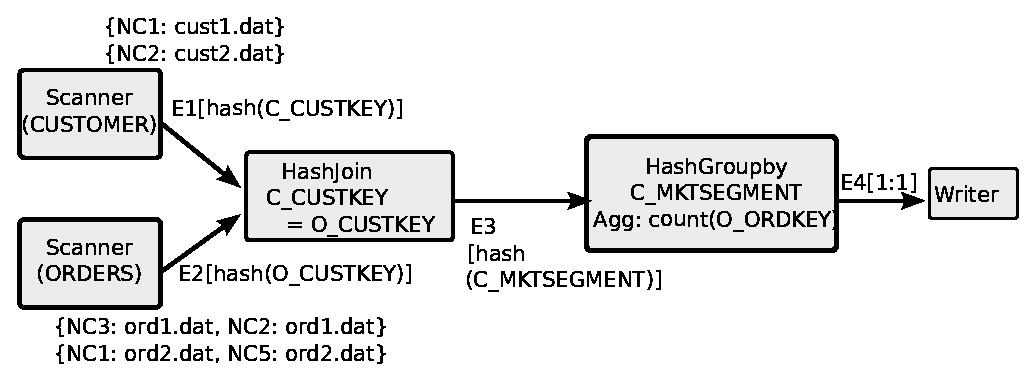
\includegraphics[scale=0.8]{images/tpch-jobspec}
\caption{Example Hyracks job specification}\label{fig:example01_spec}
\end{figure}
\vspace{-2mm}

\vspace{-2mm}
\begin{figure}[htp]
\centering
\includegraphics[scale=0.8]{images/tpch-han}
\caption{Example Hyracks Activity Node graph}\label{fig:example01_han}
\end{figure}
\vspace{-4mm}

\begin{figure*}[htp]
\centering
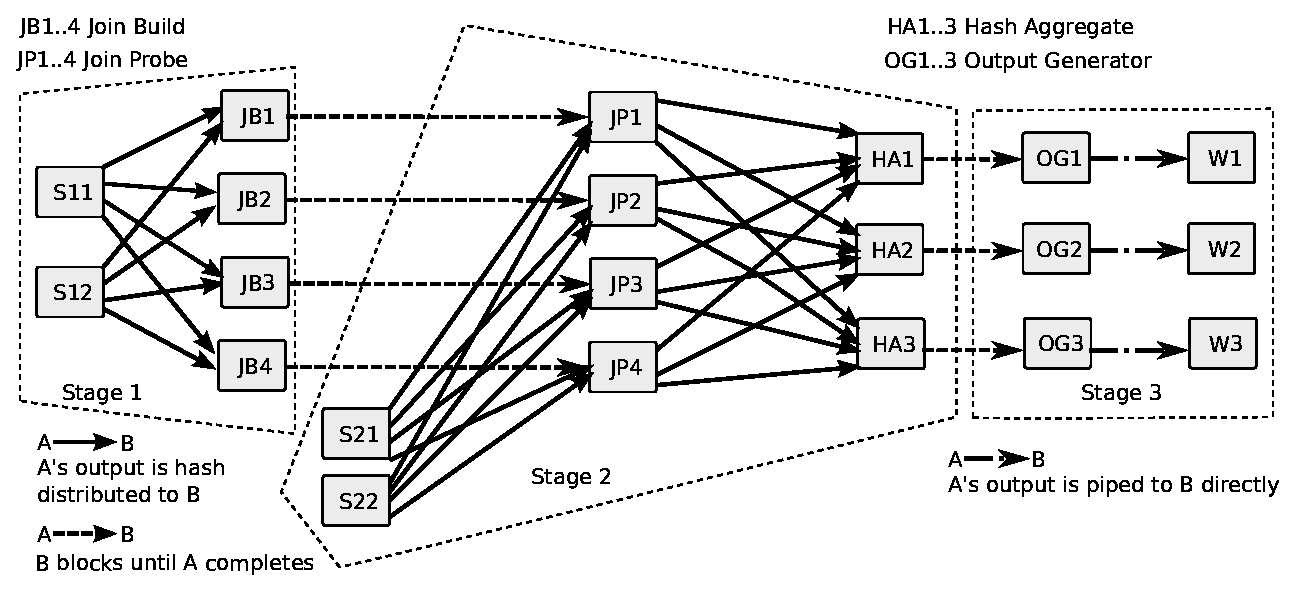
\includegraphics[scale=0.7]{images/tpch-rt}
\caption{Parallel instantiation of the example}\label{fig:example01_rt}
\end{figure*}

\subsection{High-level Architecture}

Figure \ref{fig:sysarch} provides an overview of the basic architecture of a Hyracks installation.
Every Hyracks cluster is managed by a Cluster Controller process.
The Cluster Controller accepts job execution requests from clients, plans their evaluation strategies (e.g., computing stages),
and then schedules the jobs' tasks (stage by stage) to run on selected machines in the cluster.
In addition, it is responsible for monitoring the state of the cluster to keep track of the resource loads at the various worker machines.
The Cluster Controller is also responsible for re-planning and re-executing some or all of the tasks of a job in the event of a failure.
Turning to the task execution side, each worker machine that participates in a Hyracks cluster runs a Node Controller process.
The Node Controller accepts task execution requests from the Cluster Controller and also reports on its health (e.g., resource usage levels)
via a heartbeat mechanism.  More details regarding the controller architecture and its implementation are provided in section \ref{ch:hyracks:sec:implementation}.

\begin{figure}
\centering
\includegraphics[scale=0.8]{images/architecture}
\caption{Hyracks system architecture}\label{fig:sysarch}
\end{figure}

\eat{

Hyracks runs on a shared-nothing cluster of commodity computers with local CPUs, memory, and disks. Figure \ref{fig:sysarch} shows the high level architecture of Hyracks. Some nodes are designated as ``cluster managers'' and assume the responsibility of coordinating and monitoring ``node managers''. A cluster manager is responsible for accepting job creation requests from clients, breaking a job up into discrete stages, deciding parallelization and placement of operators in each stage on the cluster, and initiating job distribution to the node managers. In addition to job management, a cluster manager also receives periodic heartbeats and resource utilization metrics from node managers which it uses in job planning and restarting failed stages. Node managers are responsible for accepting job fragments from a cluster manager and executing them using local resources. The part of a job that is deployed on a node manager is called a joblet. A joblet holds a collection of operators that perform computation on that node. Operators may exchange data with other operators on the same node (using in-process communication) or with operators on other nodes (using network communication). Whenever in-process communication can be used, Hyracks does so without the overhead of data serialization and deserialization. Periodically, node managers send heartbeat messages to cluster managers to show liveness and to relay resource utilization on the node (e.g., CPU, memory and disk activity).

\section{Hyracks jobs}

Clients specify Hyracks jobs as Hyracks Operator Descriptor nodes (HODs) connected to each other by Hyracks Connector Descriptors (HCDs) to form an acyclic directed graph. A HOD node is similar to an execution plan tree node as described in \cite{University97parallelquery}. On receiving such a job specification, the cluster manager first replaces every HOD with one or more Hyracks Activity Nodes (HAN). The process of creating a set of HANs for a HOD are delegated by Hyracks to the HOD object. This allows for an extensible operator framework.

\begin{figure}
\centering
\includegraphics[scale=0.23]{example01}
\caption{Example Hyracks job specification}\label{fig:example01_spec}
\end{figure}

Figure \ref{fig:example01_spec} shows an example specification of a job that computes the total time spent by visitors on a web site. The job gets its inputs from two logical sources called ``visits'' and ``urls''. Let us assume that ``visits'' contains (userid, page\_url, time\_spent) triplets and ``urls'' contains (page\_url, web\_site) pairs. To compute the total time spent by visitors on a website, the two inputs are joined on the ``page\_url'' fields. The output of the join is grouped on the ``web\_site'' field, and finally the ``total\_time'' field is summed up for each group. FS1 and FS2 in the figure are file scanner HODs that are parameterized with the location information of their inputs. As shown, FS1 gets its input in the form of two partitions. The first partition is replicated on the Hyracks node called NC1 in a file called visits1.dat and on NC5 in a file called vis1.dat. The second partition is available only at NC2 in a file called visits2.dat. Similarly, FS2 is configured with an input that is partitioned two ways. The two scanners feed their outputs to a Join HOD. The Join HOD in this example uses the hash-join algorithm. A sorter HOD is used to sort the join output on the web\_site field so that the grouping HOD can operate in constant space. Finally, the file writer HOD is used to produce the result.

Edges in a job specification are annotated with the type of data distribution to use. For example, E1 and E2 use a hash-based distribution on page\_url to distribute the file data to the join instances, routing data from the two sides that match on the page\_url field to the same join operator instance. Similarly, a hash distribution is used by E3 to partition data among the sorters on the web\_site field. E4 is a 1-1 edge that pipes the output of one producer to one consumer. Finally, E5 is an N-1 edge that merges the outputs of the aggregators into the file writer instance.

Figure \ref{fig:example01_han} shows the result of expansion of the HOD graph into the HAN graph. Notice that the original join HOD has been replaced with two activity nodes -- one to perform the build phase of the hash table for the hash-join, and the other to perform the probe on the hash table. A dotted arrow from the builder to the probe indicates a constraint that the probe cannot begin until the builder has completed. Hyracks guarantees that all activity nodes derived from the same HOD are co-located on the same Hyracks node at runtime so they can share information (e.g., the hash table for the join and the run files for the sorter). Note that the two inputs of the original join HOD are now connected to the HANs that actually use them. Similarly, the sort HOD has been replaced with run generation and merging activity nodes.

\begin{figure}
\centering
\includegraphics[scale=0.20]{example01_han}
\caption{Example Hyracks Activity Node graph}\label{fig:example01_han}
\end{figure}

The next step in job planning is to split it into stages. All HANs that are connected only by non-blocking edges are grouped into a stage, splitting the complete job into independent stages. The stages are planned and executed by Hyracks in such a way that all of a stage's dependencies are complete before it is executed. Hyracks plans each stage in order to decide how many instances to create (and where) for each HAN in the stage. To aid this decision, Hyracks asks HANs for any node affinities (e.g., the file scanner must indicate that it should be instantiated where some replica of each partition of the file can be accessed). The job specification can also include constraints regarding the degree of partitioned parallelism of each operator. In addition, Hyracks provides the stage planner with the ability to gather statistics (if any) from preceding stages and use them for planning. Once each stage is planned, the HAN instances are instantiated in participating Hyracks node managers to form a DAG of Hyracks Operator Nodes (HONs) at runtime. Note that the step of planning the degree of parallelism and placement of HONs is delayed until the stage is ready to run -- this allows current cluster conditions (maintained by the Resource Accountant) to play a role in the process. The HONs are responsible for consuming data from their inputs, performing computation, and sending outputs to their consuming HONs. Figure \ref{fig:example01_rt} shows the HON graph for the example. The dotted polygons bound the HONs that form a stage.

\begin{figure*}
\centering
\includegraphics[scale=0.24]{example01_rt}
\caption{Parallel instantiation of the example}\label{fig:example01_rt}
\end{figure*}

}


\section{Computational Model}
\label{ch:hyracks:sec:model}

\eat{

Computational model (3 columns)
    End user model (People, Programs) (1 Figure)
        Hyracks User model (1/2 column)
        Map-Reduce User Model (Compat layer) (1/2 column)
            Describe the TPC-H query as Map/Reduce tasks (1 Figure)
    Operator Implementor Model
        Operator Descriptor
        Operator Activity
        Operator Task
        Connector Descriptor


}

In this section, we describe the Hyracks approach to data representation and the Hyracks programming model as they pertain to two broad classes of users:
end users who use Hyracks as a Job assembly layer to solve problems, and operator implementors who wish to implement new operators for use by end users.
(Compilers for higher-level languages essentially fall into the first class of users as well.)
We also describe the built-in operators and connectors that are available as part of the initial software distribution of Hyracks.

\subsection{Data Treatment in Hyracks}

In Hyracks, data flows between operators over connectors in the form of records that can have an arbitrary number of fields.
Hyracks provides support for expressing data-type-specific operations such as comparisons and hash functions.
The type of each field is described by providing an implementation of a descriptor interface that allows Hyracks to perform serialization and deserialization.
For most basic types, e.g., numbers and text, the Hyracks library contains pre-existing type descriptors.
The Hyracks use of a record as the carrier of data is a generalization of the (key, value) concept found in MapReduce and Hadoop.
The advantage of the generalization is that operators do not have to artificially package (and repackage) multiple data objects into a single ``key'' or ``value'' object \footnote{It is interesting to note that Apache Flink (previously known as Nephele/PACTS) switched to this model from the key-value model recently.}.
The use of multiple fields for sorting or hashing also becomes natural in this model.
For example, the Hyracks operator library includes an external sort operator descriptor
that can be parameterized with the fields to use for sorting along with the comparison functions to use.
Type descriptors in Hyracks are similar to the Writable and WritableComparator interfaces in Hadoop.
However, a subtle but important difference is that Hyracks does not require the object instances that flow between operators to themselves implement a specific interface;
this allows Hyracks to directly process data that is produced and/or consumed by systems with no knowledge of the Hyracks platform or its interfaces.

\subsection{End User Model}

Hyracks has been designed with the goal of being a runtime platform
where users can hand-create jobs, like in Hadoop and MapReduce, yet at
the same time to be an efficient target for the compilers of
higher-level programming languages such as Pig, Hive, or Jaql. In
fact, the Hyracks effort was born out of the need to create an
appropriate runtime system for the ASTERIX project at UCI
\cite{asterix:website}, a project in which we are building a scalable
information management system with support for the storage, querying,
and analysis of very large collections of semi-structured nested data
objects using a new declarative query language (AQL).
Figure~\ref{fig:enduser} shows the entire AsterixDB stack.

\subsubsection{Hyracks Native User Model}

A Hyracks job is formally expressed as a DAG of operator descriptors
connected to one another by connector descriptors, as was indicated in
Figure \ref{fig:example01_spec}.  In addition to its input and output
connectors, an operator descriptor may take other parameters specific
to its operation.  For example, the ExternalSortOperatorDescriptor in
the Hyracks built-in operator library needs to know which fields in
its input record type are to be used for sorting, the comparators to
use to perform the sorting operation, and the amount of main memory
budgeted for its sorting work.

Hyracks currently allows users to choose between two ways of
describing the scheduling choices for each of the operators in a job.
One option is to list the exact number of partitions of an operator to
be created at runtime along with a list of choices of worker machines
for each partition.  Another option is just to specify the number of
partitions to use for an operator, leaving Hyracks to decide the
location assignments for each of its partitions.

\begin{figure} [htb!]
  \centering
  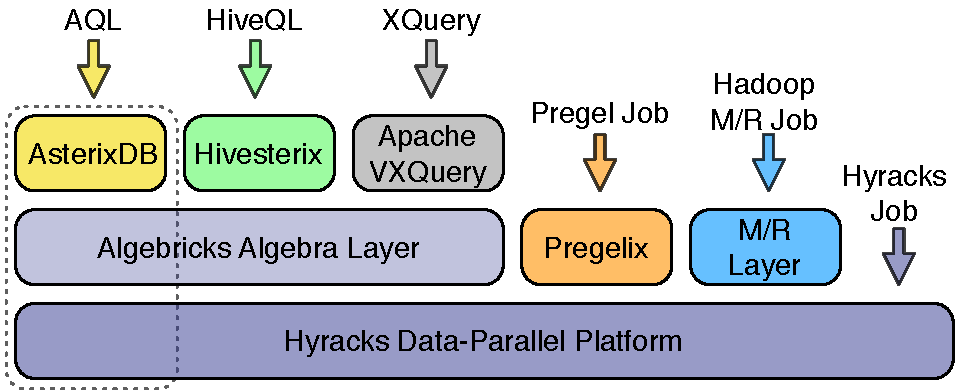
\includegraphics[width=6in]{images/asterixdb_stack}
  \caption{End User Models of Hyracks}
  \label{fig:enduser}
\end{figure}

\subsubsection{Hyracks Map-Reduce User Model}

MapReduce has become a popular paradigm for data-intensive parallel computation using shared-nothing clusters.
Classic example applications for the MapReduce paradigm have included processing and indexing crawled Web documents, analyzing Web request logs, and so on.
In the open source community, Hadoop is a popular implementation of the MapReduce paradigm that is quickly gaining traction even in more traditional enterprise IT settings.
To facilitate easy migration for Hadoop users who wish to use Hyracks, we have built a Hadoop compatibility layer on top of Hyracks.
The aim of the Hyracks Hadoop compatibility layer is to accept Hadoop jobs unmodified and run them on a Hyracks cluster.

In MapReduce and Hadoop, data is initially partitioned across the nodes of a cluster and stored in a distributed file system (DFS).
Data is represented as \texttt{(key, value)} pairs.
The desired computation is expressed using two functions:
\begin{alltt}
map    (k1,v1)       \(\rightarrow\) list(k2,v2);
reduce (k2,list(v2)) \(\rightarrow\) list(k3,v3).
\end{alltt}

A MapReduce computation starts with a map phase in which the \texttt{map} functions are applied in parallel on different partitions of the input data.
The \texttt{(key, value)} pairs output by each \texttt{map} function are then hash-partitioned on their \texttt{key}.
For each partition, the pairs are sorted by their \texttt{key} and sent across the cluster in a shuffle phase.
At each receiving node, all of the received partitions are merged in sorted order by their \texttt{key}.
All of the pair values sharing a given key are then passed to a single reduce call.
The output of each \texttt{reduce} function is finally written to a distributed file in the DFS.

To allow users to run MapReduce jobs developed for Hadoop on Hyracks, we developed two extra operator descriptors that can wrap the
\texttt{map} and \texttt{reduce} functionality.\footnote{The \texttt{combine} functionality of MapReduce is fully supported as well,
but those details are omitted here for ease of exposition.} 
The data tuples provided as input to the \id{hadoop\_mapper} operator descriptor are treated as \texttt{(key, value)} pairs and,
one at a time, passed to the \texttt{map} function.
The \id{hadoop\_reducer} operator descriptor also treats the input as \texttt{(key, value)} pairs, and groups the pairs by \texttt{key}.
The sets of \texttt{(key, value)} pairs that share the same \texttt{key} are passed, one set at a time, to the \texttt{reduce} function.
The outputs of the \texttt{map} and \texttt{reduce} functions are directly output by the operator descriptors.
To emulate a MapReduce framework we employ a sort operator descriptor and a hash-based distributing connector descriptor.

\begin{figure*}[!htb]
\centering
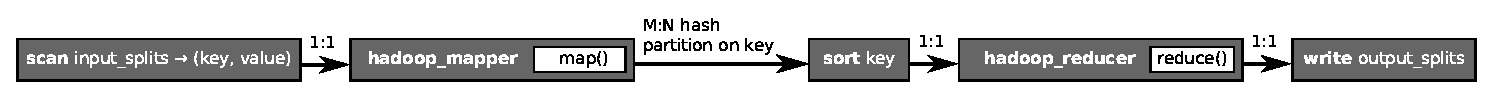
\includegraphics[scale=0.7]{images/hyrax-hadoop}
\caption{Hyracks plan for Hadoop jobs}\label{fig:hyrax-hadoop}
\end{figure*}

Figure~\ref{fig:hyrax-hadoop} shows the Hyracks plan for running a MapReduce job.
After data is read by the scan operator descriptor, it is fed into the \id{hadoop\_mapper} operator descriptor using a 1:1 edge.
Next, using an $M$:$N$ hash-based distribution edge, data is partitioned based on \texttt{key}.
(The ``$M$'' value represents the number of maps, while the ``$N$'' value represents the number of reducers.)
 After distribution, data is sorted using the sort operator descriptor and passed to the \id{hadoop\_reducer} operator descriptor using a 1:1 edge.
Finally, the \id{hadoop\_reducer} operator descriptor is connected using a 1:1 edge to a file-writer operator descriptor.

\subsection{Operator Implementor Model}

One of the initial design goals of Hyracks has been for it to be an extensible runtime platform.
To this end, Hyracks includes a rich API for operator implementors to use when building new operators.
The implementations of operators made available ``out of the box'' via the Hyracks operator library are also based on the use of this same API.

Operators in Hyracks have a three-part specification:
\begin{enumerate}
\item \emph{Operator Descriptors}: Every operator is constructed as an implementation of the Operator Descriptor interface.
Using an operator in a job involves creating an instance of the descriptor of that operator.
The descriptor is responsible for accepting and verifying parameters required for correct operation from the user during job assembly.
During the job planning phase, the descriptor is responsible for expanding itself into its constituent activities (as illustrated back in Figure~\ref{fig:example01_han}).
\item \emph{Operator Activities}: Hyracks allows an operator to describe, at a high level, the various phases involved in its evaluation.
Phases in an operator usually create sequencing dependencies that describe the order in which the inputs of the operator
are required to be made available and the order in which the outputs will become available.
Again, Figure \ref{fig:example01_han} showed the expansions for the hash-join and the hash-based grouping operators into their component activities.
As a part of the expansion, activities indicate any blocking dependencies and the mapping of overall operator inputs and outputs to the activities' inputs and outputs.
For example, when the hash-join operator is expanded, it indicates to Hyracks that its join-build activity consumes one input and its join-probe activity consumes the other.
It also indicates that its join-probe activity produces the output.
At a high level, this describes to Hyracks that the second input is not required to be available until the stage containing the join-build activity is complete.
Conversely, it also indicates that output from the join will not be available until the stage containing the join-build activity is complete.
Hyracks then uses this information to plan the stages of a job in order of necessity.
Deferring planning to the moment just prior to execution allows Hyracks to use current cluster conditions
(availability of machines, resource availability at the various machines, etc.) to help determine the schedule for a stage's tasks.
\item \emph{Operator Tasks}: Each activity of an operator actually represents a \emph{set} of parallel tasks to be scheduled on the machines in the cluster.
Tasks are responsible for the runtime aspect of the activity -- each one consumes a partition of the activity's inputs and produces a partition of its output.
The tasks corresponding to activities of the same partition of the same operator may need to share state.
For example, the join-probe task needs to be given a handle to the hashtable constructed by the join-build task.
To facilitate such state sharing, Hyracks co-locates those tasks that belong to a given partition of an activity of the same operator.
For example, in Figure \ref{fig:example01_rt}, the join-probe tasks are co-located with their corresponding join-build tasks.
Note that the join-build task will no longer be active when the join-probe task is scheduled, but Hyracks provides a shared context
for the two tasks to use to exchange the required information.
In the future we plan to explore alternative state transfer mechanisms (albeit at a higher cost),
e.g., to use when co-location is impossible due to resource constraint violations at a machine.
In terms of operator implementation, the implementor of a new operator can implement the runtime behavior
of its activities by providing single-threaded implementations of an iterator interface (a la \cite{GraefeQP}),
much as in Gamma \cite{GammaTKDE}.

\subsection{Hyracks Library}

Hyracks strongly promotes the construction of reusable operators and connectors that end users can then just use to assemble their jobs.
Hyracks, as part of its software distribution, comes with a library of pre-existing operators and connectors.
Here we briefly describe some of the more important operators and connectors.

\subsubsection{Operators}

\begin{asparaitem}
\item \emph{File Readers/Writers}:
\begin{asparaitem}
\item \emph{Line File Reader/Writer}: Reads/writes files from/to the local file system, treating a file as a sequence of lines.
\item \emph{Delimited File Reader/Writer}: Reads/writes files from/to the local file system; the files contain records separated by record delimiters,
and the records contain fields separated by field delimiters. %% The operator can be parameterized to configure its delimiters.
\item \emph{HDFS File Reader/Writer}: Reads/writes files from/to the Hadoop Distributed File system. %% The input format of the file being read/written can be configured.
%% These operators are used by the Hadoop compatibility layer to read/write files from/to HDFS, but they can also be used in the assembly of arbitrary Hyracks jobs.
\end{asparaitem}
\item \emph{Mappers}:
\begin{asparaitem}
\item \emph{Native mapper}: Used to evaluate a function once for each item in the input. Mappers can be used to implement traditional operators such
as projection and selection. %% from the relational algebra. 
%% The Mapper operator is parameterized with the function to be called for each item in its input.
\item \emph{Hadoop Mapper}: Used to call the Mapper interface in the Hadoop MapReduce library.
It is used by the compatibility layer to invoke Hadoop mappers.
\end{asparaitem}
\item \emph{Sorters}:
\begin{asparaitem}
\item \emph{In-memory Sorter}: Uses main memory to sort its input. 
% It accepts the fields in the input to use along with the comparators for those fields
% to sort the input data.
\item \emph{External Sorter}: Tries to use a main memory allocation to sort its input data, but when the input does not fit into memory,
it creates and merges runs on disk. %% It accepts the fields in the input to use along with the comparators for those fields to sort the input data (like
%% the in-memory sorter). It also accepts the maximum memory budget available for its use.
\end{asparaitem}
\item \emph{Joiners}:
\begin{asparaitem}
\item \emph{In-memory Hash Joiner}: Performs an equijoin by using memory to build a hash-table on one input and then probing the table with the other input.
%% It accepts the set of fields from each side that have to match for the join. In addition, it accepts the hash-functions to use to build and probe the hashtable and the
%% comparators to to compare the field values.
\item \emph{Hybrid Hash Joiner}: Performs an equijoin using the hybrid hash-join algorithm \cite{GraefeQP}. 
% It works with bounded memory by creating overflow partitions
% when the input data is larger than its provided memory budget. In addition to the parameters required by the In-memory Hash Joiner, it also accepts a memory budget.
\item \emph{Grace Hash Joiner}: Performs an equijoin using the Grace hash-join algorithm \cite{GraefeQP}. 
% It works with bounded memory by eagerly partitioning each input
% and then performing in-memory hash joins of the corresponding partitions of each input one-at-a-time. It requires the same parameters as the Hybrid Hash Joiner.
\end{asparaitem}
\item \emph{Aggregators}:
\begin{asparaitem}
\item \emph{Hash-based Aggregator}: Groups input data using an in-memory hash table. A custom aggregator function is invoked for each group of the input data.
%% The operator accepts the fields to use for grouping along with the hash-functions and the comparators for those fields.
\item \emph{Preclustered Aggregator}: Groups input data using very little state assuming it is already clustered on the grouping fields.
%% Similar to the hash-based aggregator, it invokes a custom aggregator function for each group.
% This operator can be used if during job assembly it is known that the input data to this operator satisfies the clustered property.
% Alternatively, one of the Sorter operators can be used to enforce this data property prior to aggregation.
\end{asparaitem}
\end{asparaitem}

\subsubsection{Connectors}
Connectors distribute data produced by a set of \emph{sender}
operators to a set of \emph{receiver} operators.
\begin{asparaitem}
\item \emph{M:N Hash-Partitioner:} Hashes every tuple produced by
  senders (on a specified set of fields) to generate the receiver
  number to which the tuple is sent.  Tuples produced by the same
  sender keep their initial order on the receiver side.
% , but there is
%   no guarantee regarding the order of tuples coming from different
%   senders.
\item \emph{M:N Hash-Partitioning Merger:} Takes as input sorted
  streams of data and hashes each tuple to find the receiver. On
  the receiver side, it merges streams coming from different senders
  based on a given comparator, thus producing ordered partitions.
\item \emph{M:N Range-Partitioner:} Takes the position $k$ of the
  partitioning field and a set of disjoint $n$ ranges, each range
  associated with one of the $n$ receiver operators. (The field at
  position $k$ must always contain integer values.) Every tuple
  produced by a sender is distributed to the receiver associated
  with the range in which the value of the $k$-th field lies.
\item \emph{M:N Replicator:} Copies the data produced by every sender
  to every receiver operator.
\item \emph{1:1 Connector:} Connects exactly one sender to one receiver
  operator. % , sending all data from the output of the sender to the input
%   of the receiver.

\end{asparaitem}

\end{enumerate}


\section{Hyracks Implementation details}
\label{ch:hyracks:sec:implementation}

In this section we describe some of the details of the Hyracks implementation.
We first describe the control portion of Hyracks, which maintains cluster membership and performs job scheduling, tracking, and recovery.
We then discuss some of the salient implementation details of modules that help Hyracks to run its operators and connectors efficiently.

\subsection{Control Layer}
\label{ch:hyracks:sec:implementation:subsec:control}

As was shown in Figure \ref{fig:sysarch}, a Cluster Controller (CC) is used to manage a Hyracks cluster.
Worker machines are added to a Hyracks cluster by starting a Node Controller (NC) process on that machine and
providing it with the network address of the Cluster Controller process whose cluster it is to join. The NC then initiates
contact with the CC and requests registration.
As part of its registration request, the NC sends details about the resource capabilities (number of cores, etc.) of its worker machine.
On successful registration, the CC replies to the NC with the rate at which the NC should provide heartbeats back to the CC to maintain continued membership in the cluster.

On receiving a job submission from a client, the CC infers the stages of the job (as was illustrated in Figures~\ref{fig:example01_han} and~\ref{fig:example01_rt}). Scheduling of a stage that is ready
to execute is performed using the latest information available about the cluster. (This may happen much later than when the job was submitted, e.g., in a long multi-stage job.)
Once it has determined the worker nodes that will participate in the execution of the stage, the CC initiates task activation on those worker nodes in parallel by pushing a
message to start the tasks. This is different from the way the Hadoop Job Tracker disseminates tasks to the Task Trackers -- Hadoop uses a pull model where the Task Trackers pull
tasks from the Job Tracker by means of a periodic heartbeat.
Although eagerly pushing job start messages increases the number of messages on the cluster, we have adopted this approach to minimize the wait time for tasks to start execution.
This becomes increasingly important as a platform tries to target short jobs.
In the future, we will explore ways of minimizing the network traffic for control messages by exploiting opportunities to piggyback multiple messages targeting the same NC.

The control logic of the Hyracks Cluster Controller was initially implemented in Overlog \cite{BOOM} using the JOL~\cite{jol:website} library. It was later reimplemented in Java due to performance concerns. We describe the Overlog implementation here since it provides insight into the behavior of the control layer in Hyracks.

Overlog is an extension of Datalog that has support
for events. Integration with JOL was convenient since both JOL and Hyracks are implemented in Java. The JOL implementation of Overlog models data as tables of records with
a declared schema. The fields in the tables can be arbitrary Java objects. JOL allows
Java code to register callbacks that are invoked by the Overlog interpreter when modifications are made to the tables. JOL also allows insertion and deletion of records
in a table from Java. At a very high level, the Java code in the CC is used to translate events from the outside world (clients submitting jobs and NC registrations/heartbeats)
into inserts and deletes on JOL tables. This action triggers the JOL interpreter to execute the JOL program which results in modifications to one or more tables that have
Java callbacks attached. When invoked with data that is inserted into or deleted from the tables by JOL, these callbacks apply the desired effects in the outside world
(e.g., by sending start/abort task messages to the NCs). Figure~\ref{fig:jolcontroller} shows the role of JOL and Java code as a controller framework.

\vspace{-1mm}
\begin{figure} [htb!]
  \centering
  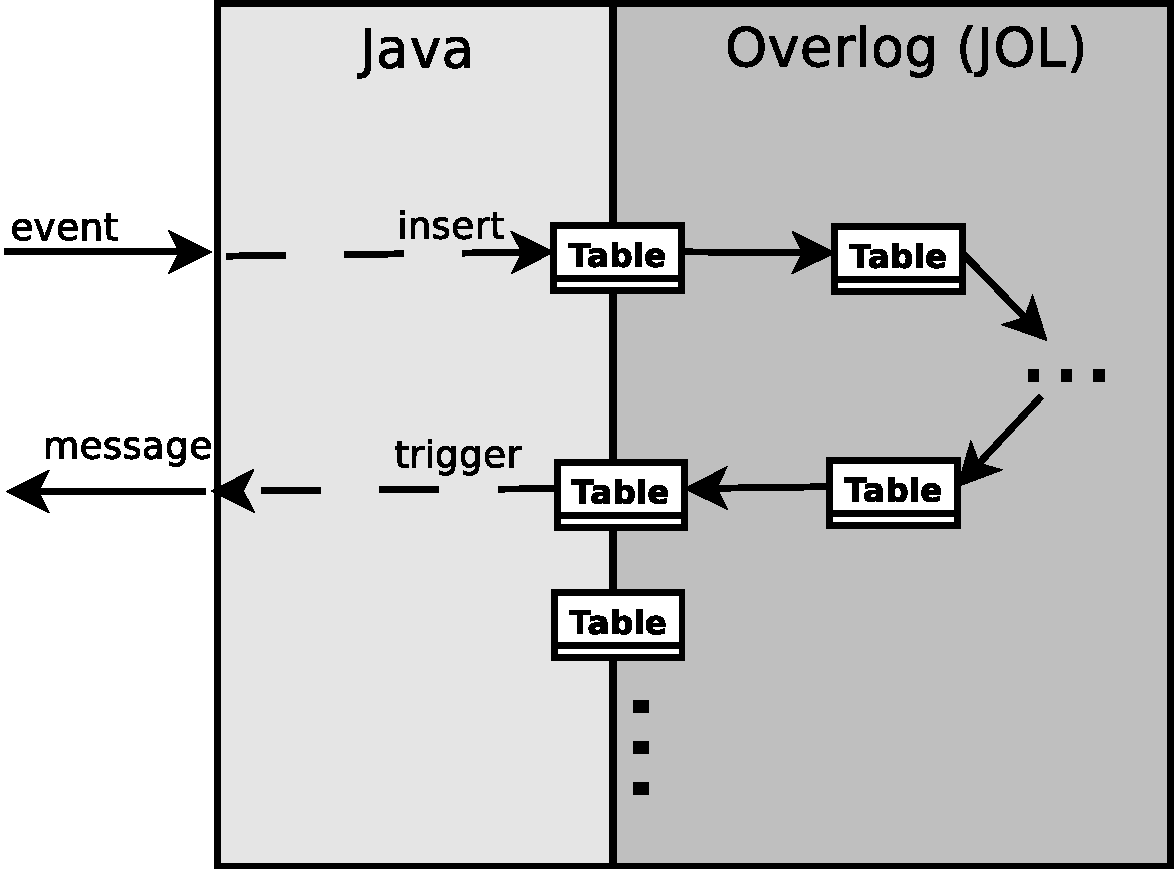
\includegraphics[scale=0.5]{images/jolcontroller}
  \caption{Mixed Java/JOL controller framework}
  \label{fig:jolcontroller}
\end{figure}
\vspace{-1mm}

Table~\ref{tbl:joltables} shows a few of the JOL tables that are relevant to identifying the stages of a Hyracks job. When a job is submitted, the CC translates the
job specification into insertions of records into the \id{operatordescriptor} (one record per Operator Descriptor) and \id{connectordescriptor} (one record per Connector
Descriptor) tables. It then visits every Operator Descriptor in the job specification and inserts a record into the \id{activitynode} table for every activity of each Operator
Descriptor. As part of the expansion of the Operator Descriptor into activities, a mapping from the Operator Descriptor inputs (and outputs) to the Operator Task inputs (and
outputs) is provided along with blocking dependencies between activities. The input/output mapping is captured in the \id{activityconnection} table while the blocking information
is captured in the \id{activityblocked} table. Once the CC has inserted records into these tables, it invokes the JOL runtime to evaluate the Overlog program.
Figure~\ref{fig:jolcontroller} shows the part of the Overlog program used by the Cluster Controller to infer stages of activities and populate the \id{activitystage\_rec} and
\id{activitystage} tables. The \id{activitystage\_rec} table is populated using rules 1 thru 4 recursively and the final result of stage assignments to activities is recorded
in the \id{activitystage} table. The rules specified in Overlog can be summarized as follows:
\begin{enumerate}
\item Rule 1: Initially assume all activities can be evaluated in the earliest stage by inserting an assignment of stage 0 to every activity in the \id{activitynode} table.
\item Rule 2: If an activity A1 must block on activity A2, and A1 is assigned a stage earlier than or the same as A2, insert a stage assignment for A1 that is one greater
than the stage assigned to A2.
\item Rules 3 and 4: If activity A1 is connected to activity A2 through a Connector Descriptor, and A1 and A2 belong to different stages, insert a stage assignment for A1 that
is the later of A1's and A2's stages. This rule occurs twice, once for A1 and once for A2, because the \id{connectordescriptor} table captures a one-way connection whereas
for the stage assignment we concern ourselves with the existence of a connection. Intuitively, if we wish to co-schedule (for pipelining) the activities connected by a data
flow connector, they will both need to be assigned to the latter of the stages to which they belong.
\item Rule 5: Finally, the actual stage number associated with an activity is the maximum over all of the stage number assignments and is captured in the \id{activitystage} table.
\end{enumerate}

\begin{table*}
\center
\caption{Tables identifying stages of a Hyracks job.}\label{tbl:joltables}
\begin{footnotesize}
\begin{tabular}{|l|l|}
\hline
Table Name & Table Attributes \\
\hline \hline
\id{operatordescriptor} & JobId, OperatorDescriptorId, OperatorDescriptor  \\
\hline
\id{connectordescriptor} & JobId, ConnectorDescriptorId, SourceOperatorId, \\ & SourcePort, TargetOperatorId, TargetPort, ConnectorDescriptor \\
\hline
\id{activitynode} & JobId, OperatorDescriptorId, ActivityId, Activity \\
\hline
\id{activityconnection} & JobId, OperatorDescriptorId, OperatorPort, \\ & Direction, ActivityId, ActivityPort \\
\hline
\id{activitystage} & JobId, OperatorDescriptorId, ActivityId, StageNumber \\
\hline
\id{activityblocked} & JobId, BlockingOperatorDescriptorId, BlockingActivityId, \\ & BlockedOperatorDescriptorId, BlockedActivityId \\
\hline
\end{tabular}
\end{footnotesize}
\end{table*}

\eat{
\begin{table*}
\caption{Fragment of Overlog program for inferring stages of activities.}
\label{fig:jolexample}
\begin{footnotesize}
\begin{tabular}{|l|l|l}
activitystage\_rec & (JobId, OpId, ActivityId, 0) \pdef 
     activitynode(JobId, OpId, ActivityId,\longunderscore); & (1)\\
activitystage\_rec & (JobId, OpId2, ActivityId2, Stage) \pdef 
     activitystage\_rec(JobId, OpId1, ActivityId1, Stage1), & (2) \\
&     activitystage\_rec(JobId, OpId2, ActivityId2, Stage2),\\
&     activityblocked(JobId, OpId1, ActivityId1, OpId2, ActivityId2), \\
&     Stage2 \leq Stage1 \ \ \{\ \ Stage := Stage1 + 1;\ \  \}; \\
activitystage\_rec & (JobId, OpId2, ActivityId2, Stage) \pdef 
    activitystage\_rec(JobId, OpId1, ActivityId1, Stage1), & (3) \\
  &  activitystage\_rec(JobId, OpId2, ActivityId2, Stage2), \\
  &  activityconnection(JobId, OpId1, Op1Port, Dir.OUT, ActivityId1, \longunderscore), \\
  &  activityconnection(JobId, OpId2, Op2Port, Dir.IN, ActivityId2, \longunderscore), \\
  &  connectordescriptor(JobId, \longunderscore\,,, OpId1, Op1Port, OpId2, Op2Port, \longunderscore), \\
  &  Stage1 \neq  Stage2 \ \  \{\ \ Stage := java.lang.Math.max(Stage1, Stage2);\ \ \}; \\
activitystage\_rec & (JobId, OpId1, ActivityId1, Stage) \pdef 
     activitystage\_rec(JobId, OpId1, ActivityId1, Stage1), & (4) \\
   & activitystage\_rec(JobId, OpId2, ActivityId2, Stage2), \\
   & activityconnection(JobId, OpId1, Op1Port, Dir.OUT, ActivityId1, \longunderscore), \\
   & activityconnection(JobId, OpId2, Op2Port, Dir.IN, ActivityId2, \longunderscore), \\
   & connectordescriptor(JobId,\longunderscore\,, OpId1, Op1Port, OpId2, Op2Port, \longunderscore), \\
   &  Stage1 \neq  Stage2 \ \  \{\ \ Stage := java.lang.Math.max(Stage1, Stage2);\ \ \}; \\
activitystage & (JobId, OpId, ActivityId, max<Stage>) %\pdef 
     activitystage\_rec(JobId, OpId, ActivityId, Stage); & (5)
\end{tabular}
\end{footnotesize}
\end{table*}
}
The scheduling and fault-recovery logic was also implemented in Overlog using the general principles described above. Although Overlog was very expressive and could succinctly represent most logic that was necessary for performing scheduling actions and handling faults, it had some major drawbacks. The simple act of assigning a monotonically increasing integer to each item in a collection, which can be implemented to have linear complexity in any imperative language, is a quadratic operation in Overlog. Assigning such an integer, involves repeatedly computing the maximum number assigned so far, and assigning one more than that number to the ``next'' item in the collection. Quite a few places in the Hyracks control layer needed the assignment of sequential numbers (for example, the assignment of partition ids to the Hyracks Operator Nodes), and the quadratic complexity of this operation created a performance bottleneck when the collection sizes were large. This directly translated to longer scheduling times for large jobs. Since there was no easy way to work around this issue (and it was not our focus, at that time), we decided to reimplement the control layer in Java to recapture all the lost performance in an expedient manner. It would be interesting to investigate ways of adding efficient mechanisms for number assignment to a language like Overlog.

\subsection{Task Execution Layer}

Once a stage of a Hyracks job becomes ready to run,
the CC activates the stage on the set of NCs that have been chosen to run the stage and then waits until the stage completes or until an NC failure is detected.
In the remainder of this section we explore the task activation process and then discuss some details of the implementation of the data-processing and data-movement
aspects of Tasks and Connectors, respectively.

\subsubsection{Task Activation}

When a stage becomes ready to run, the Cluster Controller sends messages to the Node Controllers participating in that stage's execution to perform task activation in three
steps.
\begin{enumerate}
\item \emph{Receiver Activation}: The CC initiates a ReceiverActivation request to every NC that participates in a stage's execution. Each NC, on receipt of this request,
creates the Task objects that have been designated to run at that NC (as determined by the scheduler). For each Task that accepts inputs from other
Tasks, it creates an endpoint that has a unique network address. The mapping from a Task object's input to the endpoint address is relayed back to the CC as the response to
this request.
\item \emph{Sender-Receiver Pairing}: Once the CC receives the ReceiverActivation responses containing local endpoint addresses from the NCs, it merges all of them together to
create a global endpoint address map. This global map is now broadcast to each NC so that the send side of each Task object at that NC knows the network addresses of its
consumer Tasks.
\item \emph{Connection Initiation}: Once pairing has completed on all NCs, the CC informs all of the NCs that the Tasks can be started.
\end{enumerate}

\subsubsection{Task Execution and Data Movement}

The unit of data that is consumed and produced by Hyracks tasks is called a Frame.
A frame is a fixed-size (configurable) chunk of contiguous bytes. A producer of data packs a frame
with a sequence of records in a serialized format and sends it to the consumer who then interprets the records. Frames never contain partial records; in other words, a record
is never split across frames. A naive way to implement tasks that process records is to deserialize them into Java objects and then process them. However, this 
has the potential to create many objects, resulting in more data copies (to create the object representation) and a burden on the garbage collector (later) to reclaim
the space for those objects. To avoid this problem, Hyracks provides interfaces for comparing and hashing fields that can be implemented to work off of the binary data
in a frame. Hyracks includes implementations of these interfaces for the basic Java types (String, integer, float, etc.). Hyracks also provides Task implementors with helper
functions to perform basic tasks on the binary data such as to copy complete records, copy specific fields, and concatenate records from source frames to target frames.

A task's runtime logic is implemented as a push-based iterator that receives a frame at a time from its inputs and pushes result frames to its consumers. Note that the task-runtime only
implements the logic to process streams of frames belonging to one partition without regards to any repartitioning of the inputs or outputs that might be required. Any
repartitioning is achieved by using a Connector. The connector runtime has two sides, the send-side and the receive-side. There are as many send-side instances of a connector
as tasks in the producing activity, while there are as many receive-side instances as tasks in the consuming activity. The send-side instances are co-located with the
corresponding producer tasks, while the receive-side instances are co-located with the consuming tasks. When a send-side instance of a connector receives a frame from its
producing task, it applies its redistribution logic to move records to the relevant receive-side instances of the connector. For example, the M:N hash-partitioning
connector in Hyracks redistributes records based on their hash-value. The send-side instances of this connector inspect each record in the received frame, compute
the hash-value, and copy it to the target frame meant for the appropriate receive-side instance. When a target frame is full, the send-side instance sends the frame to
the receive-side instance. If the send-side and receive-side instances of a connector are on different worker machines (which is most often the case), sending a frame
involves writing it out to the network layer. The network layer in Hyracks is responsible for making sure that the frame gets to its destination.

In order to use network buffers efficiently on the receive-side of a connector, Hyracks allows the connector implementation to specify the buffering strategy for received
frames. Figure~\ref{fig:networkbuffers} shows two buffering strategies that could be chosen by a connector. If the receive-side logic of a connector does not differentiate
between the frames sent by the various send-side instances, it can choose to use one network buffer for all senders. On the other hand, if the connector's logic requires
treating frames from different senders separately, it can use one network buffer per send-side instance. For example, the M:N hash-partitioning connector does not differentiate
frames based on their senders. However, an M:N sort-merge connector, which assumes that frames sent by a sender contain records that are pre-sorted, needs to decide which
sender's frame to read next in order to perform an effective merge.

\vspace{-1mm}
\begin{figure} [htb!]
  \begin{minipage}[b]{0.38\linewidth}
  \centering
  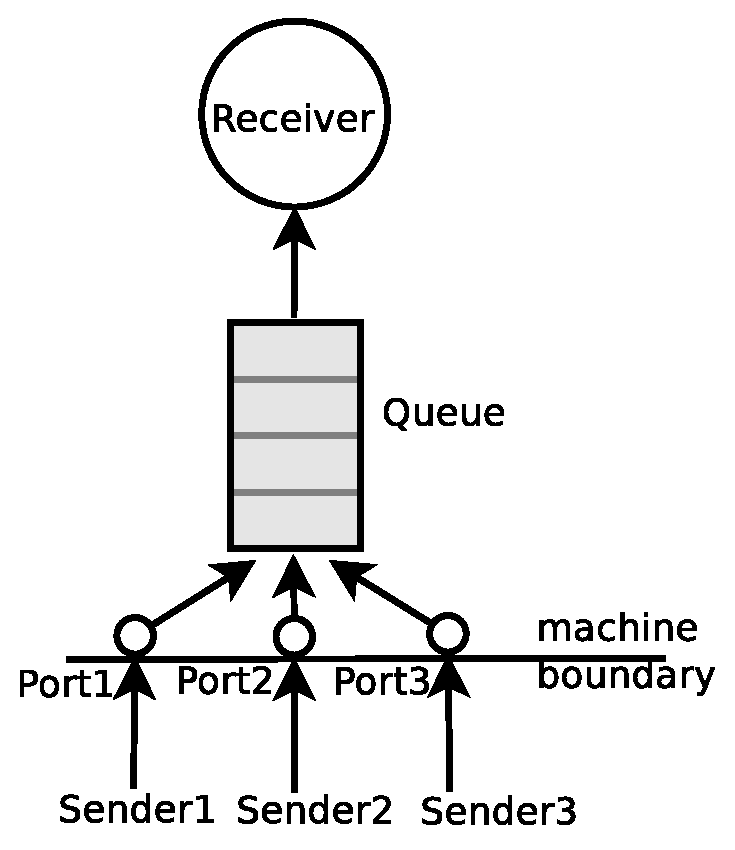
\includegraphics[scale=0.3, trim=10 10 30 10]{images/connector1}
  \legend{Shared buffer}
  \end{minipage}
  \begin{minipage}[b]{0.55\linewidth}
  \centering
  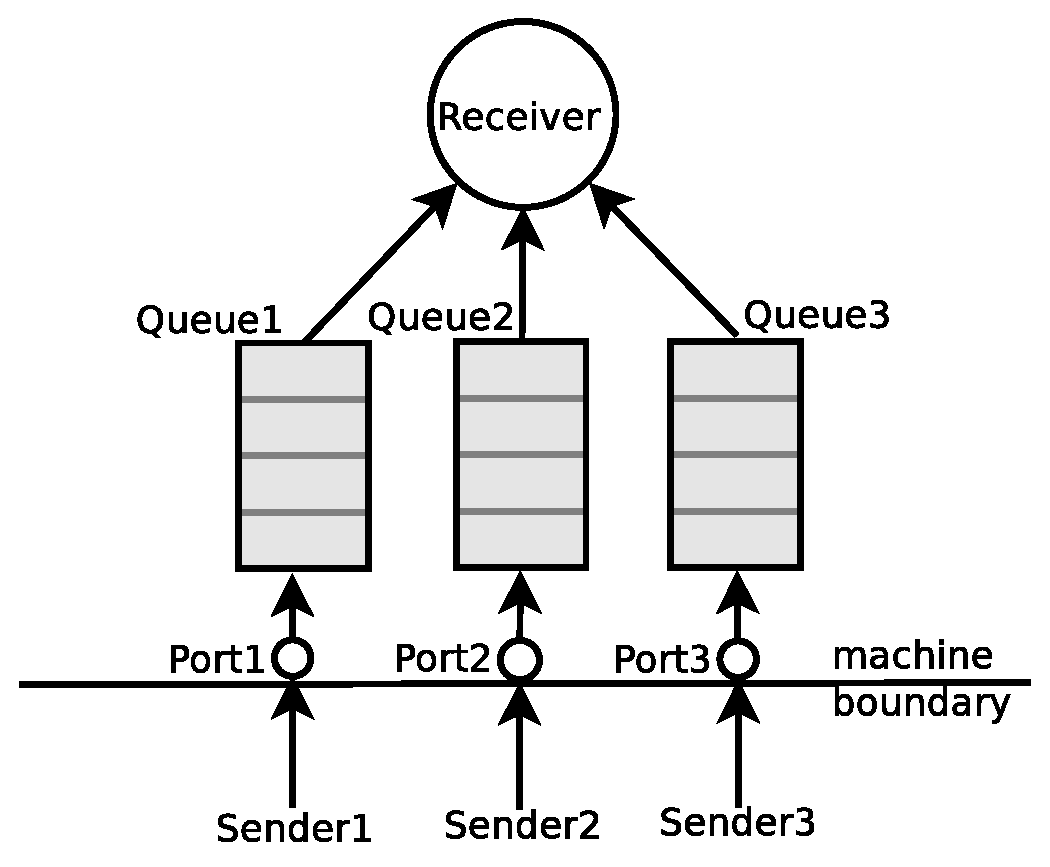
\includegraphics[scale=0.3, trim=7 10 40 10]{images/connector2}
  \legend{One buffer per sender}
  \label{subfig:networkbuffers}
  \end{minipage}
  \caption{Buffering strategies for connectors.}\label{fig:networkbuffers}
\end{figure}
\vspace{-1mm}

\section{Experimental Results}
\label{ch:hyracks:sec:experiments}

In this section we report the results of early performance comparisons (erformed in 2011) of Hadoop and Hyracks as data-intensive computing platforms. First, we compare the performance
of jobs written using the
MapReduce paradigm by running them on Hadoop and running the same jobs unchanged on Hyracks using its Hadoop compatibility layer. Next, we show the difference in performance
that results from not being limited to the MapReduce model in Hyracks. Finally, we explore the performance of Hadoop and Hyracks when node failures occur by using a simple model
for generating failures.

For all of the experiments shown in this section, we used a cluster
of ten IBM machines each with a 4-core Xeon 2.27 GHz CPU, 12GB of main memory, and four locally attached 10,000 rpm SATA drives. The same cluster was used for Hyracks
as well as Hadoop. The Hadoop version used was 0.20.1 (the latest release available when these experiments were performed, in 2011).

\subsection{MapReduce on Hyracks}

In this section, we compare the running times of three very different kinds of jobs (K-Means clustering, a TPC-H style query, and Set-Similarity Joins) on Hadoop
versus on Hyracks using the compatibility layer.

\subsubsection{K-Means}
K-Means is a well known clustering algorithm that tries to find clusters given a set of points. Mahout \cite{mahout:website} is a popular open source project
that includes a Hadoop implementation of the K-Means algorithm as MapReduce jobs.
The clustering problem
consists of grouping a set of $n$ points into $k$ clusters
$\{C_i\}_{i=1,k}$ with centers $\{\mu_i\}_{i=1,k}$, such that each
point is assigned to the cluster with the closest center. The K-Means
MapReduce implementation~\cite{nips06-mapreducemulticore} starts with a randomized
algorithm (called canopy computation) to heuristically determine the number of
clusters that the K-Means algorithm must try to find.
The canopy MapReduce job finds $k$ points to serve as initial centroids of the
$k$ clusters that will then be refined by subsequent iterations of the K-Means algorithm.
Each iteration of the K-Means algorithm is also implemented as a MapReduce job. The Map phase
scans over the set of data points in the input and finds their closest centroid $\mu_j$ among
the $k$ centroids computed in the previous step. Once the closest centroid is found,
that input point is deemed to belong to cluster $j$. The output of the Map phase is
regrouped by the cluster assignment of each point and routed to the Reducers.
The Reduce phase computes a new cluster centroid for each of the $k$ clusters by averaging the coordinates of all points assigned to that cluster.

\begin{figure} [htb!]
  \centering
  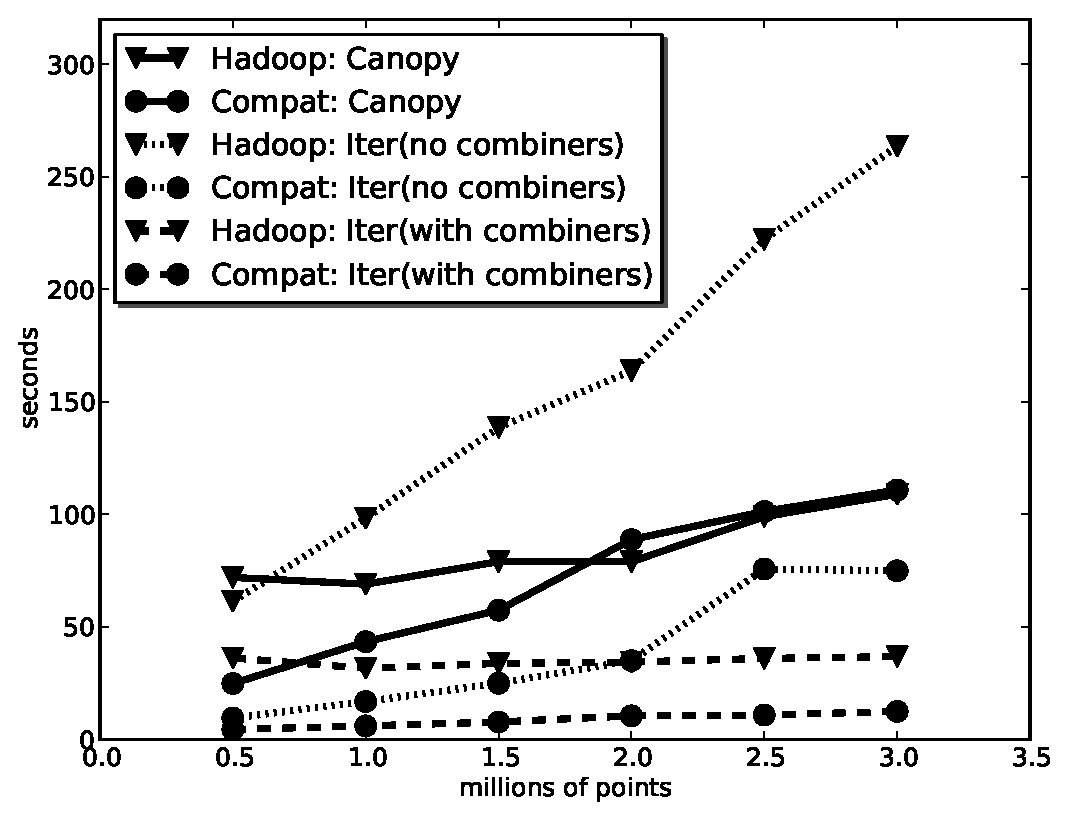
\includegraphics[scale=0.6]{images/KMeans}
  \caption{K-Means on Hadoop and Hyracks}
  \label{fig:kmeans}
\end{figure}

In Figure~\ref{fig:kmeans} we show separately the time taken by the canopy computation
phase and by the iterations for K-Means on both systems. We further explore the efficiency tradeoffs
of Hyracks vs. Hadoop as a data-platform by presenting the average running-time of the iterations both with and
without combiners in the two systems. Turning off combiners for the iterative part
of the K-Means algorithm increases dramatically the amount of data that is moved from the
Map phase to the Reduce phase (although it does not change the final result).

From Figure~\ref {fig:kmeans} we see that the canopy computation phase benefits the least from
running on Hyracks since it is mostly CPU intensive. This phase initially (for 0.5
and 1 million points) shows faster time to completion on Hyracks.
However, as the size of the data grows from 1.5 to 3 million points, the two lines
essentially converge.  This is because Hyracks runs the same CPU-intensive user functions
that Hadoop runs, and hence there is not much room for improvement there.
On the other hand, when much of a job's time is spent in re-organizing data
by partitioning and sorting, running the MapReduce job on Hyracks performs better.
The K-Means iteration results clearly show this behavior.  
This improvement owes itself to the more efficient nature of the data-movement
layer that forms the foundation for the Hyracks operators and connectors.

In Hadoop, moving data from the mappers to the reducers is performed rather inefficiently.
All data from the mappers is written to disk before it is moved to the reducer side.
When a reducer is notified of a mapper's completion, it initiates a pull of its
partition using HTTP. The resultant near-simultaneous fetch requests from all reducers to the mappers
leads to disk contention on the Map side as the reducers try to read all of the requested
partitions from disk; there is also a surge in network traffic created by such
simultaneous requests \cite{conf/nsdi/CondieCAHES10}.

In Hyracks, data is instead pushed from the producers to the consumers in the form of fixed
sized chunks (on the order of 32KB) incrementally, as they are produced. This leads to a much smoother
utilization of the network throughout the processing time of the producer. Also, since the
producer decides when a block is sent out, the aforementioned disk contention issue does not arise
in Hyracks.



\subsubsection{Set-Similarity Joins}

Set-Similarity Joins match data items from two collections that are deemed to be similar to each other according to a similarity function. Work reported in \cite{FuzzyJoinMR}
performed an extensive evaluation of algorithms for computing such joins using the MapReduce framework. From that work we took the best MapReduce algorithm to compare
its performance on Hadoop vs. on Hyracks using the Hadoop compatibility layer. This ``fuzzy join'' computation requires three stages of MapReduce jobs, as shown in Figures
\ref{fig:fuzzyjoin-tokensbasic}, \ref{fig:fuzzyjoin-ridparisimporved}, and \ref{fig:fuzzyjoin-recordparisbasic}.
The first stage tokenizes the input records and produces a list of tokens ordered by frequency using two MapReduce jobs. The second stage (one MapReduce job) produces
record-id pairs of similar records by reading the original data and using the tokens produced in the first stage as auxiliary data. The final stage of SSJ computes
similar record pairs from the record-id pairs from Stage 2 and the original input data using two MapReduce jobs.
We refer the reader to \cite{FuzzyJoinMR} for more details about the algorithm.

\begin{figure}
    %% \begin{figure}
    \center
    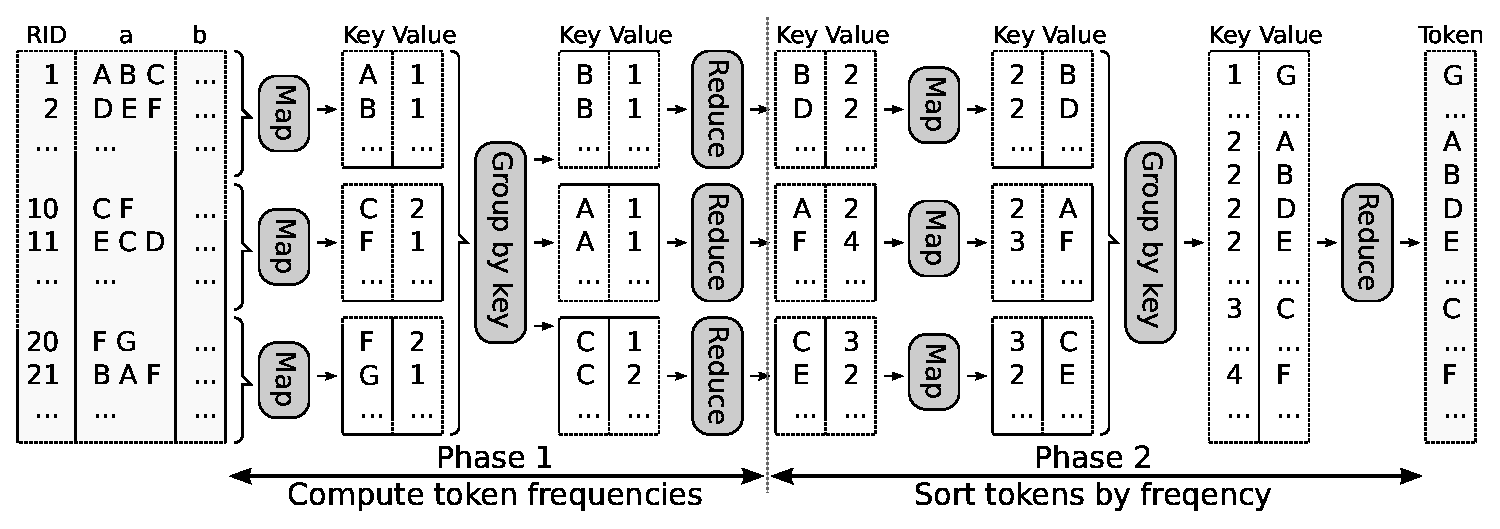
\includegraphics[scale=0.7]{images/fuzzyjoin-tokensbasic}
    \caption{Example data flow of Stage 1 of Set-Similarity
      Joins. (Basic Token ordering for a self-join on attribute
      ``\texttt{a}''.)}
    \label{fig:fuzzyjoin-tokensbasic}
    %% \end{figure}

    %% \begin{figure}
    \center
    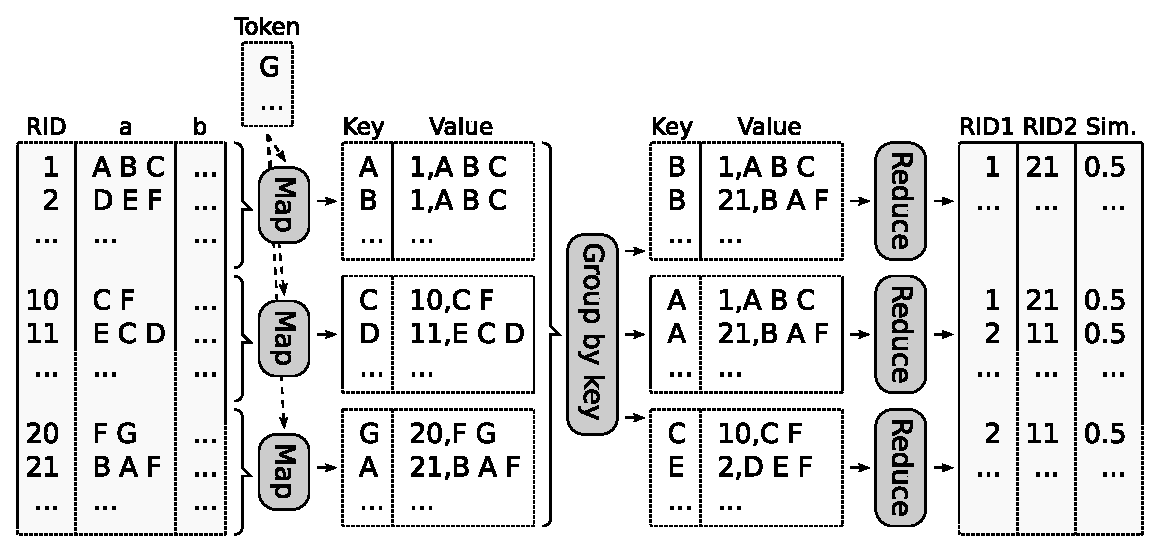
\includegraphics[scale=0.7]{images/fuzzyjoin-ridpairsimproved}
    \caption{Example data flow of Stage 2 of Set-Similarity
      Joins. (Basic Kernel for a self-join on attribute ``\texttt{a}''.)}
    \label{fig:fuzzyjoin-ridparisimporved}
    %% \end{figure}
\end{figure}

    \begin{figure}
    \center
    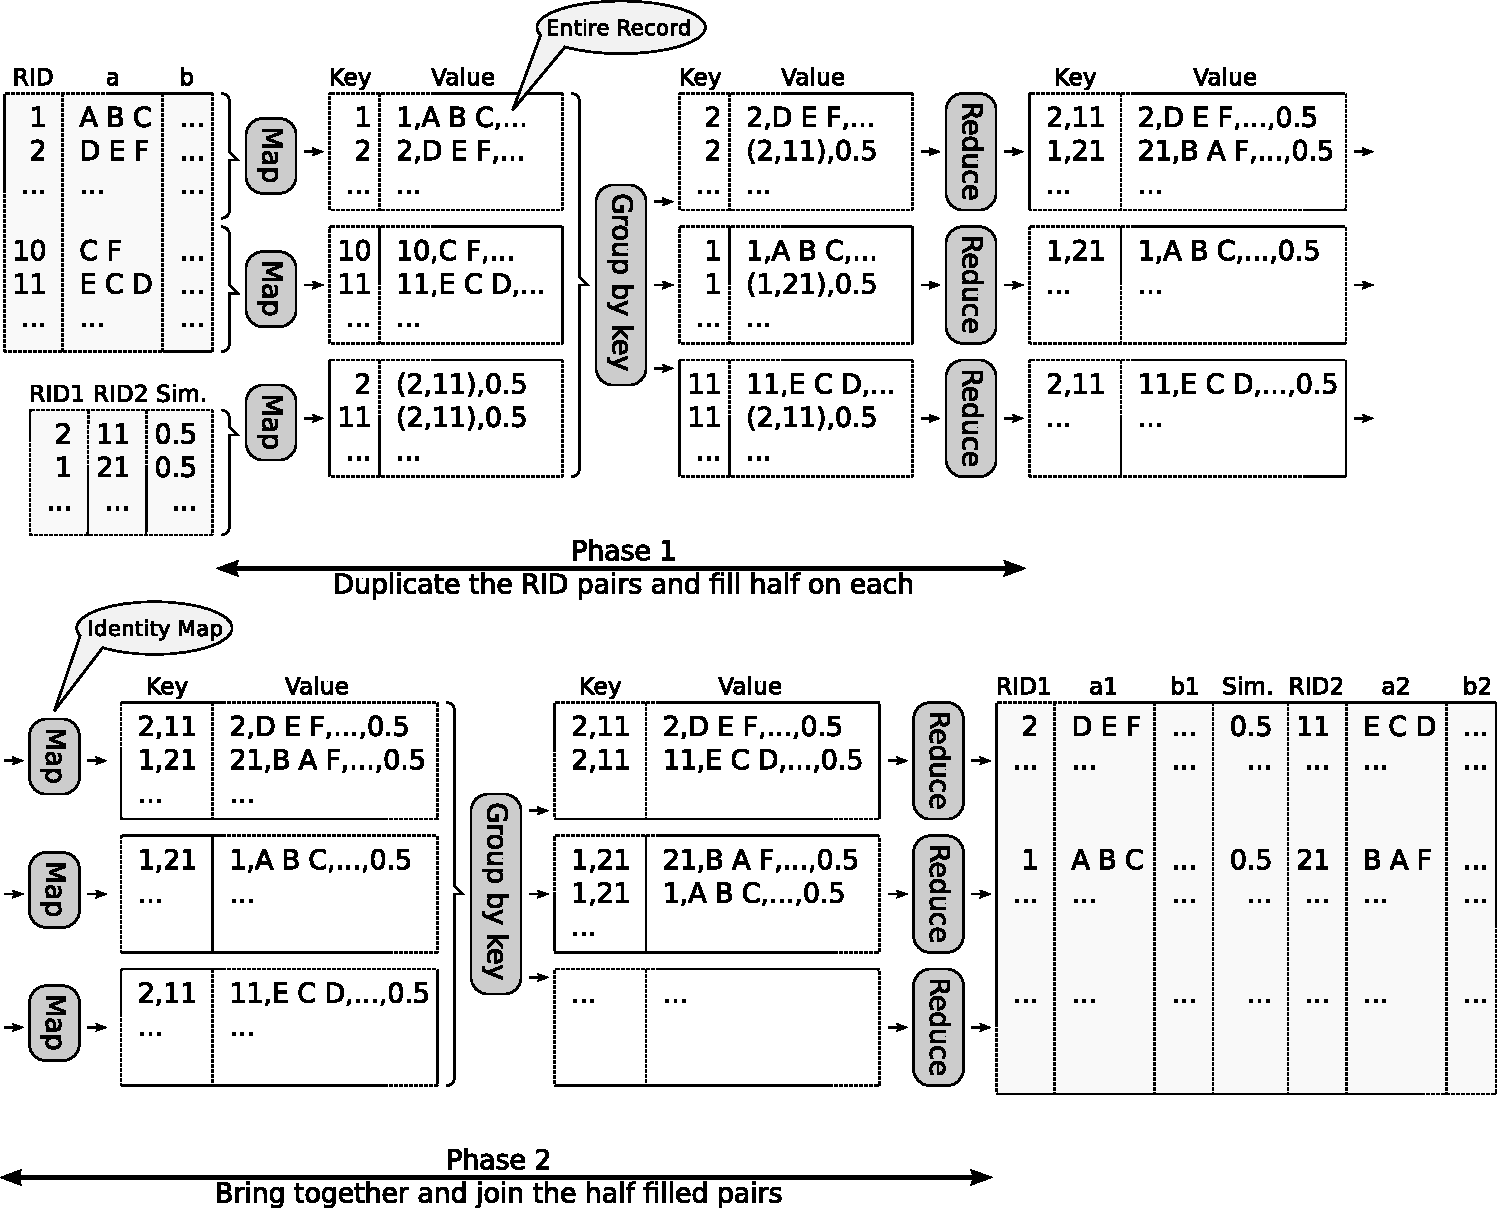
\includegraphics[scale=0.7]{images/fuzzyjoin-recordpairsbasic}
    \caption{Example data flow of Stage 3 of Set-Similarity Joins using
      Basic Record Join for a self-join case. ``\texttt{a1}'' and
      ``\texttt{a2}'' correspond to the original attribute
      ``\texttt{a}'', while ``\texttt{b1}'' and ``\texttt{b2}''
      correspond to attribute ``\texttt{b}''.}
    \label{fig:fuzzyjoin-recordparisbasic}
    \end{figure}
For comparing the performance of Set-Similarity Joins (SSJ), we used the algorithm shown in the figures to find publications with similar titles in the DBLP
dataset~\cite{dblp:xml} by performing a
join of the DBLP data with itself. In order to test performance for different sizes of data, we increased the DBLP data sizes to 5x, 10x, and 25x over the original dataset
(which contains
approximately 1.2M entries) using the replication scheme of~\cite{FuzzyJoinMR}. Table~\ref{tbl:sizeup-fuzzyjoins} shows the running times for the three
stages of the SSJ algorithm on the three different sizes of data. The row labeled ``Hadoop'' represents the time taken to run each stage as a Hadoop job; ``Compat'' shows the
time taken to run the same MapReduce jobs using the compatibility layer on Hyracks (Please ignore the row labeled ``Native'' for now; it will be explained shortly).

\begin{table} [htb!]
\caption{Size-up for Parallel Set-Similarity Joins (10 nodes)}\label{tbl:sizeup-fuzzyjoins}
\center
\begin{tabular}{cl||c|c|c|c}
                     &        & Stage 1 & Stage 2 & Stage 3 & Total time\\
\hline\hline
\multirow{3}{*}{5x}  & Hadoop &   75.52 &  103.23 &   76.59 &  255.34 \\
                     & Compat &   24.50 &   38.92 &   23.21 &   86.63 \\
                     & Native &    11.41 &   32.69 &    9.33 &   53.43 \\
\hline
\multirow{3}{*}{10x} & Hadoop &   90.52 &  191.16 &  107.14 &  388.82 \\
                     & Compat &   42.15 &  128.86 &   38.47 &  209.49 \\
                     & Native &   16.14 &   81.70 &   14.87 &  112.71 \\
\hline
\multirow{3}{*}{25x} & Hadoop &  139.58 &  606.39 &  266.26 & 1012.23 \\
                     & Compat &  105.98 &  538.74 &   60.62 &  705.34 \\
                     & Native &   34.50 &  329.30 &   27.88 &  391.68 \\
\end{tabular}
\end{table}

In the column labeled ``Stage 1'' in Table~\ref{tbl:sizeup-fuzzyjoins}, we see that the MapReduce jobs running on Hadoop scale smoothly with increasing data sizes.
The Hadoop compatibility layer on Hyracks
also shows this trend. However, the job running on Hyracks is faster because it benefits from two improvements: low job startup overhead and more efficient data movement
by the infrastructure.
Hyracks uses push-based job activation, which introduces very little wait time between the submission of a job by a client and when it begins running on the node controllers.

In the column labeled ``Stage 2'' in Table~\ref{tbl:sizeup-fuzzyjoins}, we observe a near constant difference between the running times of Hadoop and Hyracks. This is because
most of the time in this stage is spent in the Reducer code that uses a quadratic algorithm~\cite{FuzzyJoinMR} to find matching records.
The key thing to note is that
most of
the work in this stage is done in the Reduce phase in user-defined code, so the only improvement we can expect is due to lower overhead of the infrastructure.

The column labeled ``Stage 3'' in Table~\ref{tbl:sizeup-fuzzyjoins}, shows that at 5x data size, the ratio of the Hadoop completion time to the Hyracks compatibility
layer completion time is 3.3; the ratio drops to about 2.8 at the 10x
data size. As the amount of data grows to 25x, we see the compatibility layer completing about 4 times faster than Hadoop.
This is because Stage 3 performs two ``joins'' of the record-ids with the original data to produce similar-record-pairs from the similar-record-id-pairs that were produced by
the previous
stage. Every join step reshuffles all of the original input data from the Map to the Reduce phase, but the output of the join is fairly small. Most of the work is thus
performed in moving the data (as the Map and Reduce code is fairly simple). At smaller data sizes, Hadoop times are dominated by startup overhead, while for larger data
sizes the dominating factor is data redistribution. 

\subsubsection{TPC-H}

The TPC-H query is the query from the Hyracks running example that was introduced in Section~\ref{ch:hyracks:sec:overview:subsec:example}. Figure~\ref{fig:tpchmr} shows the structure of the two
MapReduce jobs corresponding to the running example from Figure~\ref{fig:example01_spec}.

\begin{figure} [htb!]
  \centering
  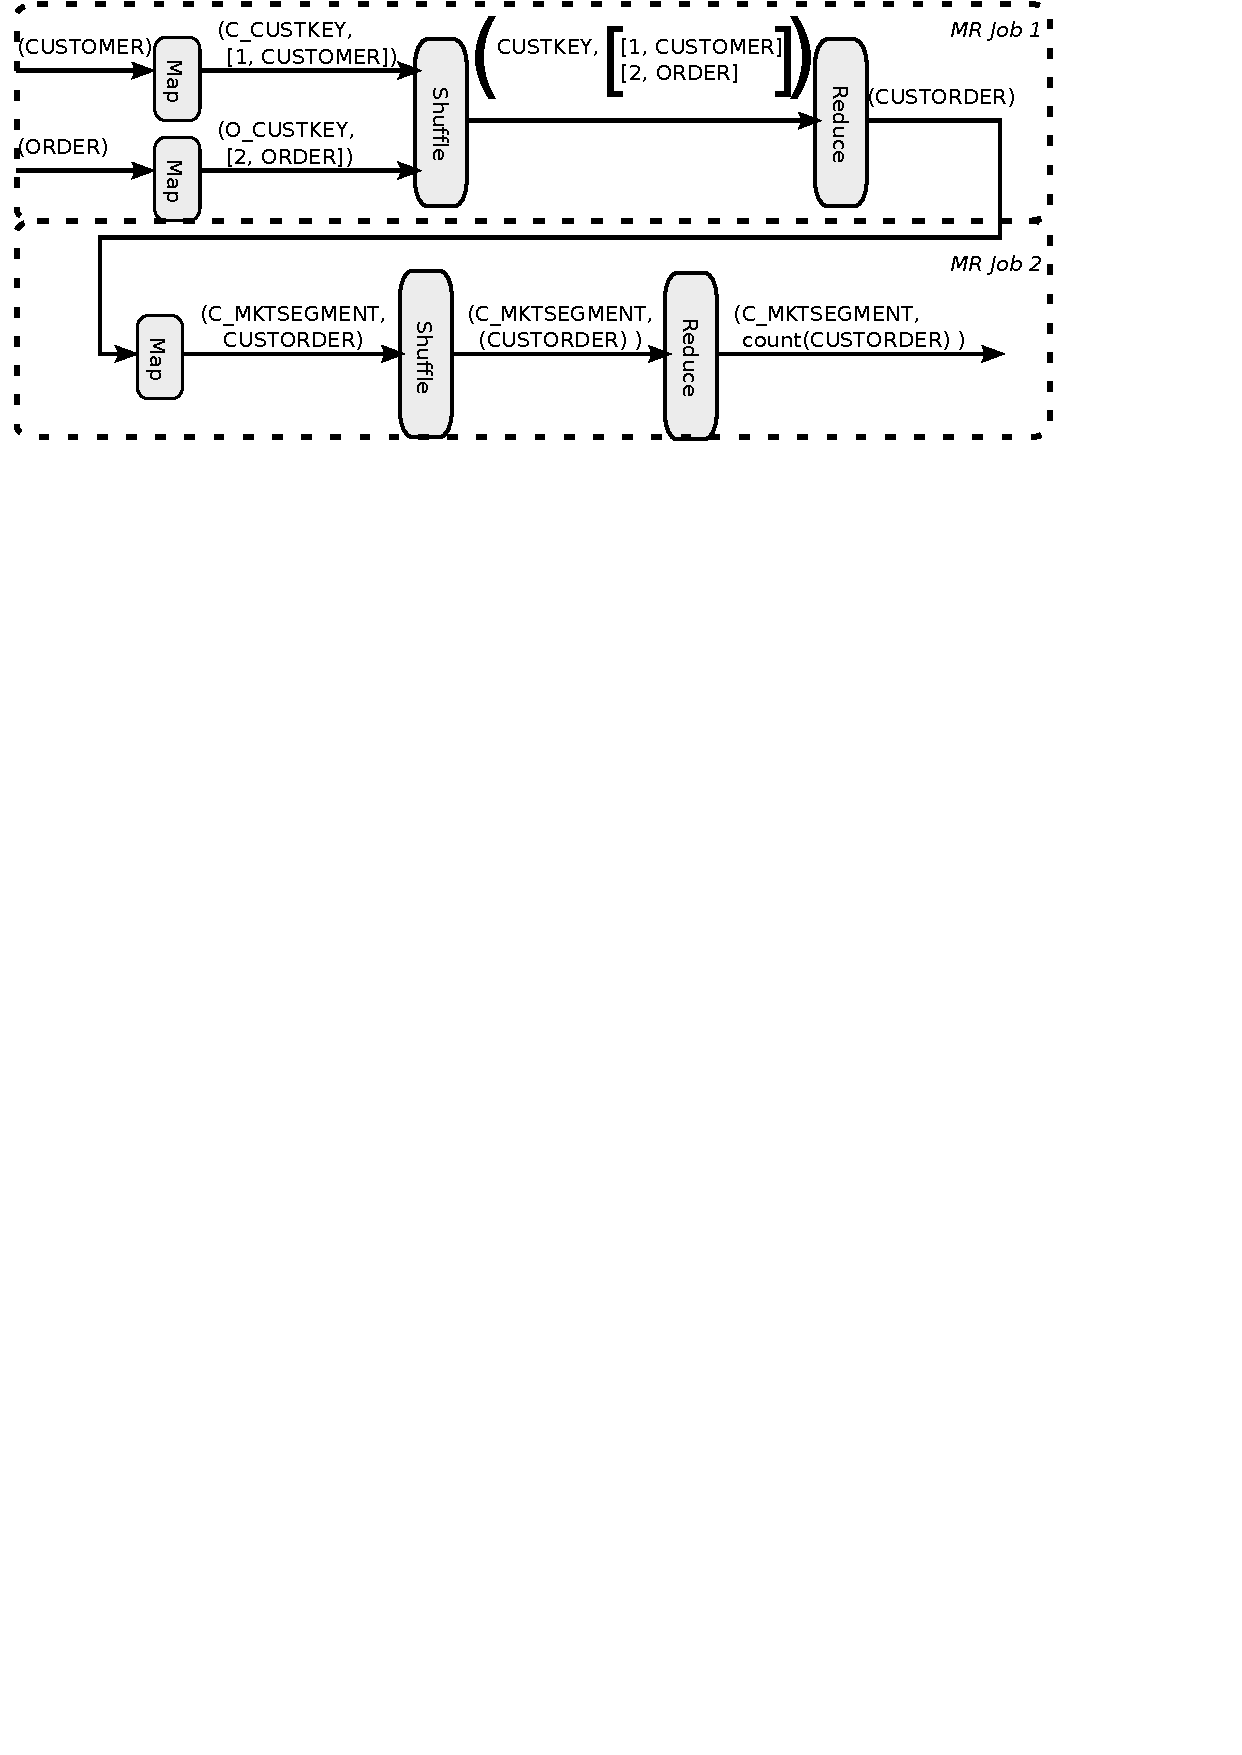
\includegraphics[scale=1]{images/tpch-mr}
  \caption{Hadoop implementation of TPC-H query from Fig.~\ref{fig:example01_spec}.}
  \label{fig:tpchmr}
\end{figure}

The first MapReduce job in Figure~\ref{fig:tpchmr} performs the join using the tagged-join method described in \cite{MapReduceBenchmark}, while the second job computes
the aggregation.  The Mapper of the first job generates the value field as a tagged output that indicates whether the record is
from the CUSTOMER source or the ORDER source. The associated key is generated by extracting the C\_CUSTKEY field if it is a customer record or the O\_CUSTKEY if it
is an ORDER record.
The Reducer of the join job then receives all records (both CUSTOMER and ORDER) that match on the join key. The Reducer function then generates the CUSTOMER-ORDER pairs
to be sent to the output.
The data generated from this first MapReduce job is used as the input for the second MapReduce job, which performs the aggregation step by grouping
the data on the value of the C\_MKTSEGMENT field and then computing the desired count. The Mapper of this job produces the value of C\_MKTSEGMENT as the key and the
CUSTOMER-ORDER pair as the value. The Reducer thus receives
a list of CUSTOMER-ORDER pairs for the same value of C\_MKTSEGMENT that it then counts. The final query output is emitted as a pair of C\_MKTSEGMENT and count values.

As with the other tasks, we measured the end-to-end response time of the jobs by running them on Hadoop and comparing that with the time it took to run the
same MapReduce jobs on Hyracks using the compatibility layer. In addition to the standard configuration of running the two MapReduce jobs sequentially, with HDFS used to store
the intermediate join result, we also executed the compatibility layer with ``pipelining'' between jobs turned on. In this case the join job pipelines data to the aggregation
MapReduce job without the use of HDFS.

As we see from Figure~\ref{fig:tpch-sizeup}, TPC-H on Hadoop takes about 5.5 times the time taken by the compatibility
layer on Hyracks for smaller data sizes (scale 5). Job start-up overhead in Hadoop is responsible for this slowness. As data sizes grow, we observe that the running times for
Hadoop and the compatibility
layer grow super-linearly. This is not surprising since there are two sort steps involved, one in the first MapReduce job to perform the join of CUSTOMER and ORDER data, and
the second to perform aggregation in the second MapReduce job. The result of the join is quite large, and hence a substantial amount of time is spent in partitioning and
sorting. To measure the time spent in writing the join results to HDFS and reading it back in, we also ran in compatibility mode with pipelining turned on. We observe from
Figure~\ref{fig:tpch-sizeup} that I/O to and from HDFS adds significant overhead. At scale 40, the compatibility layer takes about 133 seconds (about 25\% longer
than the pipelined execution).
Note however that all of the MapReduce running times exhibit a super-linear curve owing to the sort operations (We will ignore the ``Hyracks Native'' curve for now).

\begin{figure} [htb!]
  \centering
  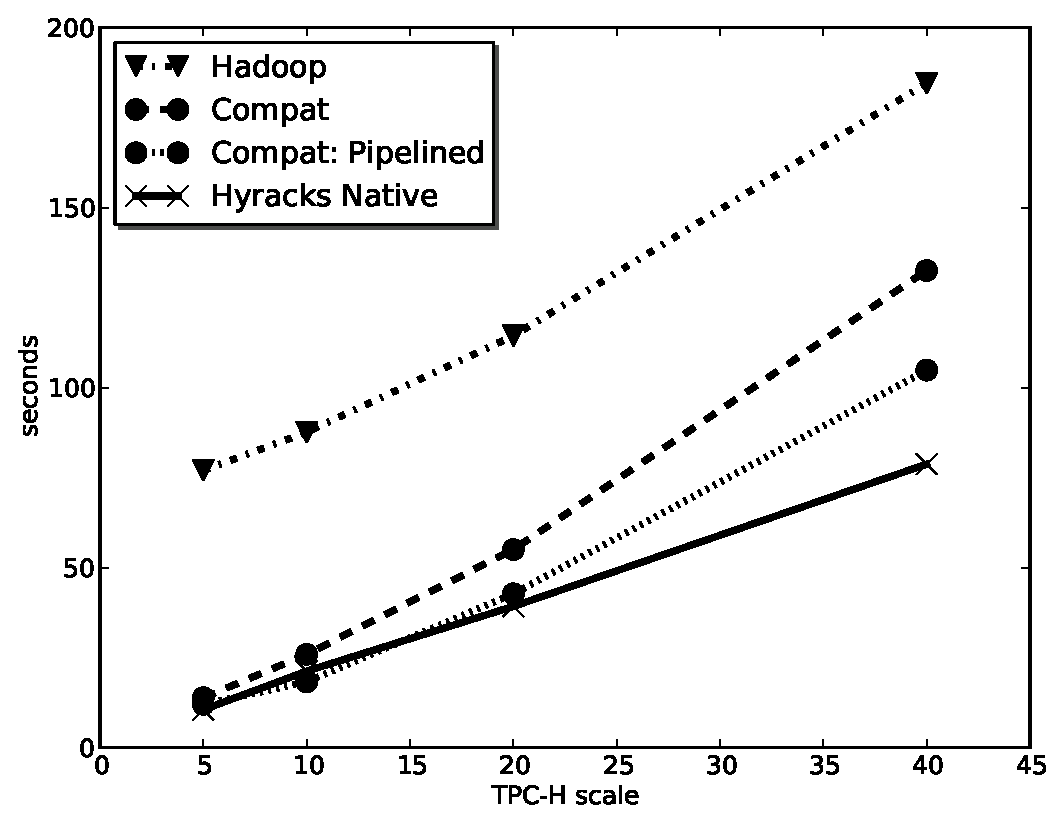
\includegraphics[scale=0.6]{images/tpch-sizeup}
  \caption{TPC-H query from Fig.~\ref{fig:example01_spec} with Hadoop and Hyracks.}
  \label{fig:tpch-sizeup}
\end{figure}

\subsection{Beyond MapReduce}

We now show the results of running two experiments to study the performance improvements obtainable in Hyracks by not being restricted to the MapReduce programming model.
We present results for Set-Similarity Joins and the TPC-H join/aggregate example query.

\subsubsection{Set-Similarity Joins (Take 2)}

\begin{figure} [htb!]
    %% \begin{figure}
    \center
    \includegraphics[scale=0.5]{images/fuzzyjoin-hyrax-stage1}
    \caption{Hyracks-native plan for Stage 1 of Set-Similarity Self-Joins.}
    \label{fig:fuzzyjoin-hyrax-stage1}
    %% \end{figure}
    %% \begin{figure}
    \center
    \vspace{.5em}
    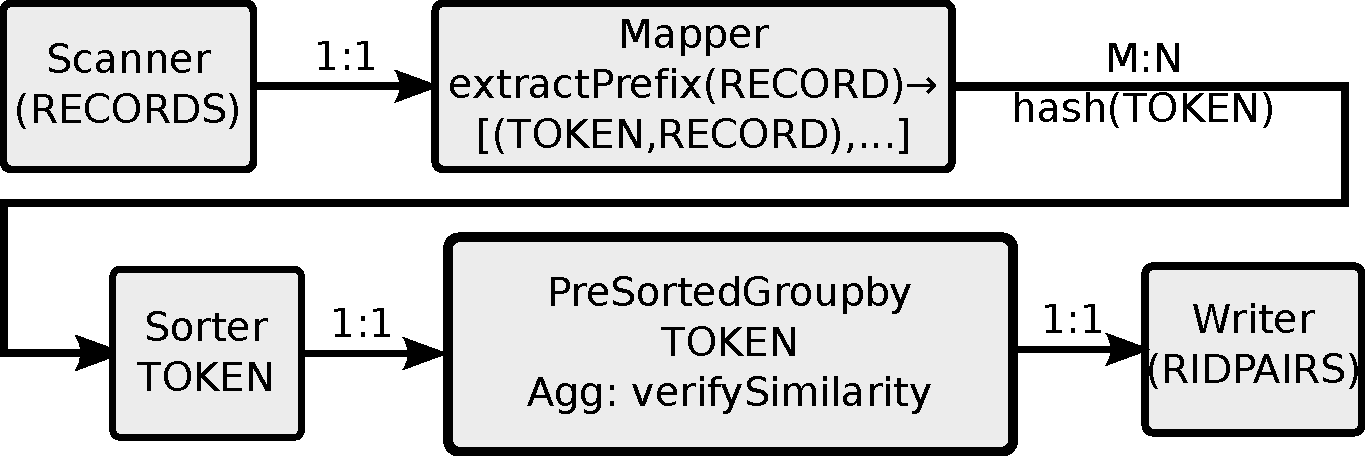
\includegraphics[scale=0.5]{images/fuzzyjoin-hyrax-stage2}
    \caption{Hyracks-native plan for Stage 2 of Set-Similarity Self-Joins.}
    \label{fig:fuzzyjoin-hyrax-stage2}
    %% \end{figure}
    %% \begin{figure}
    \center
    \vspace{.5em}
    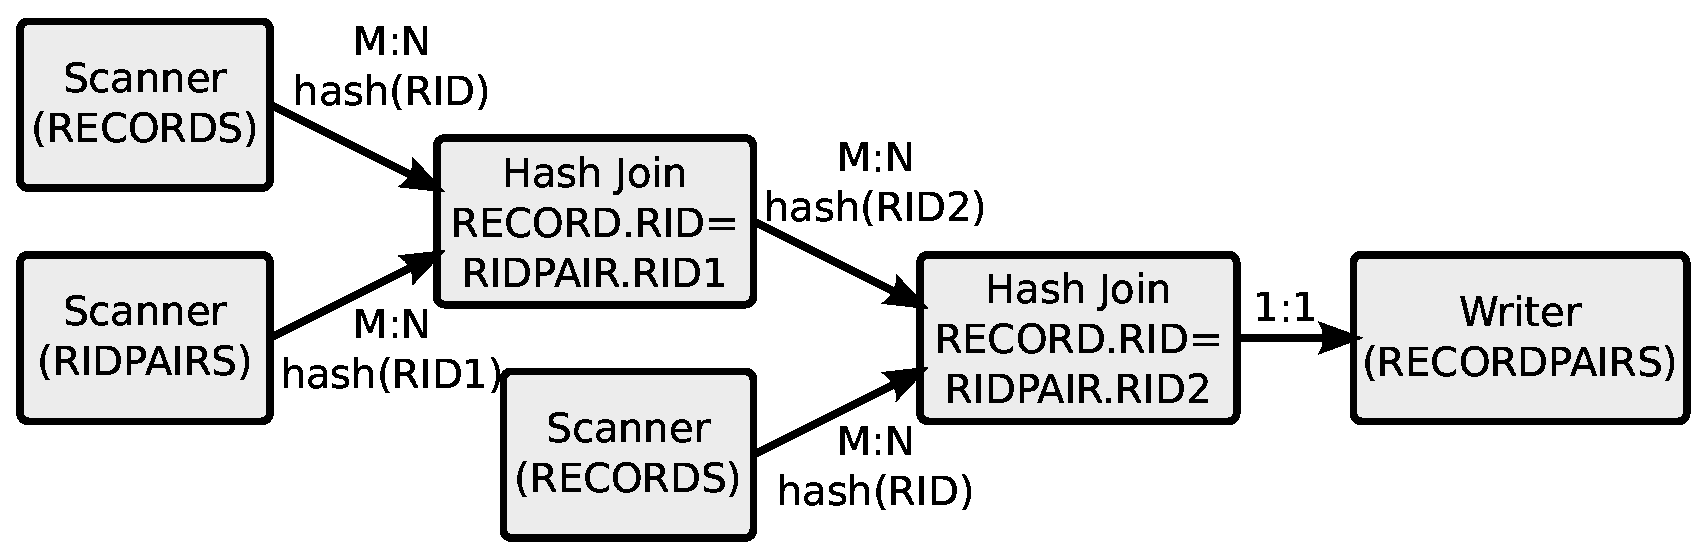
\includegraphics[scale=0.5]{images/fuzzyjoin-hyrax-stage3}
    \caption{Hyracks-native plan for Stage 3 of Set-Similarity Self-Joins.}
    \label{fig:fuzzyjoin-hyrax-stage3}
    %% \end{figure}
\end{figure}

Figures \ref{fig:fuzzyjoin-hyrax-stage1}, \ref{fig:fuzzyjoin-hyrax-stage2}, and \ref{fig:fuzzyjoin-hyrax-stage3} show the native Hyracks job specifications to
implement the three stages of the Hadoop based Set-Similarity Join examined in the previous subsection.

In Table~\ref{tbl:sizeup-fuzzyjoins}, the row labeled ``Native'' shows the time
required by the Hyracks jobs to perform Set-Similarity Joins. We can now compare these
times to those that we examined previously. These faster Native times are due in part to the savings
already discussed, but here we also see additional algorithmic benefits. Stage 1 benefits the most
from the Native formulation due to the use of hash based grouping, which does not need
to sort the input data like in Hadoop. Stage 3, in the Native case, benefits from using
hash join operators that perform the joins by building a hash-table on one of their inputs
and then probing the table using the other input. This strategy is cheaper than first
sorting both inputs on the join key to bring the matching values from both the sides
together (which is what happens in Hadoop). In Stage 2, we used sort-based grouping since it performed
slightly better than its hash-based counterpart. Usually, hash-based aggregation works well
for traditional aggregates when grouping is performed on relatively low cardinality attributes, as
compression is achieved by the aggregation. In the case of Stage 2, however, the grouping
operation is used to separate the input into groups without applying an incremental aggregation function.
The sort operator in Hyracks implements the ``Poor man's normalized key'' optimization mentioned
in~\cite{GraefeCPUCache} which can be exploited when building Hyracks Native jobs.
This optimization helps in terms of providing cheaper comparisons and better cache locality.  
After sorting, the ``aggregation'' function performs a quadratic scan of the items
within each group. This is seen in Table~\ref{tbl:sizeup-fuzzyjoins} as a super-linear growth in the completion time for Stage 2.

In summary, we see that the Native formulation of Set-Similarity Joins run about 2.6 to 4.7
times faster than their MapReduce formulation running on Hadoop and about 1.6 to 1.8
times faster than running the same MapReduce jobs on Hyracks using its compatibility layer.

\subsubsection{TPC-H (Take 2)}

We now compare the two MapReduce TPC-H implementations with the native Hyracks implementation.
The ``Hyracks Native'' line in Figure~\ref{fig:tpch-sizeup} shows the results of natively running the TPC-H query in Figure~\ref{fig:example01_spec}.
Notice that for large data the TPC-H query executes on Hyracks much faster than the MapReduce counterparts on Hadoop or on Hyracks via the compatibility layer. As in the
native expression of
Set-Similarity Joins, this is due in part to the fact that the TPC-H query uses hash-joins and hash-based aggregation. In addition, Hyracks does not need to materialize
intermediate results between the
joiner and the aggregator. In contrast, since Hadoop accepts one MapReduce job at a time, it needs to persist the output of the Join job for this example in HDFS. To
minimize the ``damage'' caused by this materialization on the Hadoop completion time, we set the replication factor in HDFS to 1 (meaning no replication). We observe that
the Hyracks job scales linearly with growing data size since all operations in the pipeline have linear computational complexity for the memory and data sizes
considered here.

To conclude, Hyracks is a more efficient alternative to Hadoop for MapReduce jobs, and even greater performance benefits can be achieved by not being restricted
to the MapReduce programming model. Here we have compared the performance characteristics of Hadoop and Hyracks in detail for K-Means clustering, Set-Similarity joins, and an
example TPC-H query. We have measured even greater benefits for simpler jobs. For example, the standard Hadoop Word-Count MapReduce job on 12 GB of data ran approximately twice
as fast on Hyracks using the compatibility layer than on Hadoop, and a Native Word-Count implementation on Hyracks ran approximately 16 times as fast as the Hadoop
MapReduce version.

\subsection{Fault Tolerance Study}

A system designed to run on a large number of commodity computers must be capable of detecting and reacting to possible faults that might occur during its regular operation.
In this part of the thesis, we perform a very simple experiment to illustrate the fact that, while being able to run jobs through to the end despite failures is valuable,
doing so by being pessimistic and ever-prepared for incremental forward-recovery is not a general ``right'' answer. Hadoop uses a naive strategy based on storing all
intermediate
results to durable storage before making progress. While such a naive strategy is a safe first approach, we wish to begin exploring the path of applying more
selective fault-tolerance. Hyracks is in a better position to exploit operator and connector properties to achieve the same degree of fault tolerance while doing less
work along the way. As our first step in this direction, the Hyracks fault-tolerance strategy that we use for the experiment in this section is to simply restart
all jobs impacted by failures.
Although such a strategy cannot be the only one in a system like Hyracks, we believe that this is actually an effective strategy for smaller to medium-sized jobs.

We used the TPC-H example query shown in Figure~\ref{fig:example01_spec} on data scale 40 for this experiment. In our experimental
set-up, we had the client submit the same job
request over and over again in an infinite loop without any think time and we measured the observed completion time for every request.
Separately, we killed a randomly chosen cluster
node at regular intervals. In different runs of the experiment, we changed the mean time between failures from 100 seconds to 1600 seconds. The same experiment was
performed with the jobs running on Hyracks and then with the corresponding jobs running on Hadoop. Figure~\ref{fig:tpch-fault-tolerance} shows the observed request
completion time (retry times included) for the two systems for different MTBF (mean time between failure) values. The data inputs to the jobs in both systems were
replicated so that a node failure could still allow progress of the job.

\begin{figure} [htb!]
  \centering
  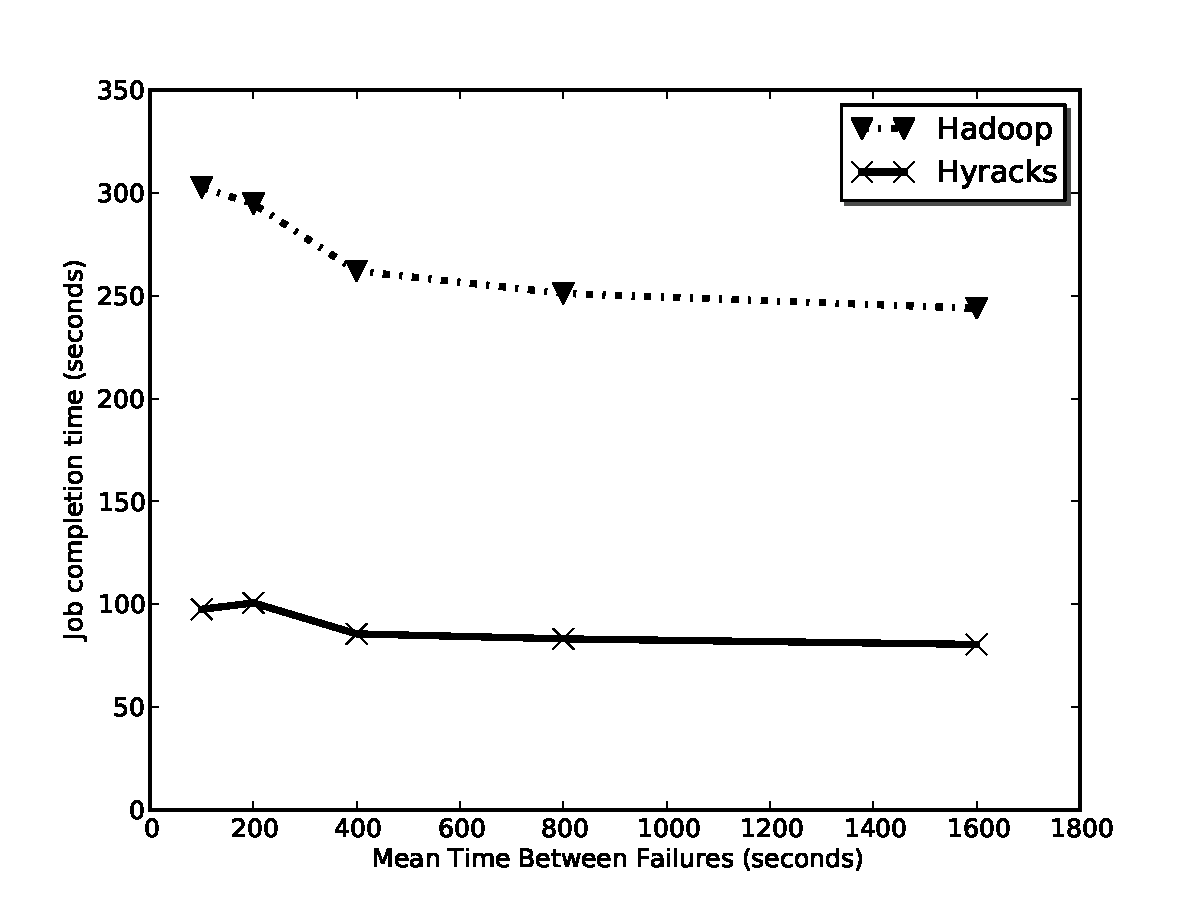
\includegraphics[scale=0.6]{images/tpch-fault-tolerance}
  \caption{TPC-H query from Fig.~\ref{fig:example01_spec} in the presence of failures.}
  \label{fig:tpch-fault-tolerance}
\end{figure}

In Hadoop in order to provide as much isolation from failures as possible, every
map task writes its output to the local disk before its data is made available to the reducer side. On the reducer side, every partition fetched from every map task is written
to local disk before a merge is performed. The goal of the extra I/O in Hadoop is to make sure that at most one task needs to be restarted when a failure occurs. In the current
implementation of Hyracks, however, data is pipelined from producers to consumers, so a single failure of any one node requires a restart of all of the operators that are 
currently part of the same pipelined stage.

We observe from Figure~\ref{fig:tpch-fault-tolerance} that Hyracks runs the TPC-H job to completion faster even when failures are injected into the cluster very frequently.
Note also that, since a given Hyracks job runs to completion much faster than the ``fault-tolerant'' Hadoop job, a given Hyracks job is less likely to be hit by a failure
during its execution in the first place.

As we mentioned earlier, a strategy
that requires a complete restart cannot be the only fault recovery strategy in a system. If the mean time between failures is less than the mean time to complete a
job, then such a job
may never complete.

\section{Conclusion}

This chapter described the design and implementation of Hyracks. Hyracks was built from the group-up to serve as an efficient, parallel, dataflow runtime platform. Based on the the performance comparison performed with the Hadoop MapReduce layer for a variety of tasks, we can conclude that the design philosophy of Hyracks has merit. Since its availability as an open-source project, Hyracks has also proven to be a successful research platform that has been used to build various other systems on top of. For example, Hyracks has been used to build the Pregelix layer to perform graph analytics at massive scale, which in turn has been used to solve graph problems arising in the field of genetics.

\chapter{Algebricks: A Data Model-Agnostic Compiler Backend}
\label{ch:algebricks}

In this chapter, we describe the design and implementation of the Algebricks layer. As we started to build the AQL compiler for the AsterixDB platform, we realized that having a generic compiler framework to compile declarative languages to evaluate using a parallel dataflow platform like Hyracks would be useful to the community at large. Based on prior research in the area of extensible systems and query algebras, we designed the Algebricks library to help query language implementors avoid spending time building a lot of boiler plate code that goes into implementing a full-fledged compiler. Algebricks, along with Hyracks, enables query language implementors to have a complete parallel query compiler in a matter of days.


\section{The Algebricks Framework}\label{sec:algebricks-fw}

Algebricks is an 
%data-model-agnostic, 
algebraic layer for parallel query
processing and optimization.
To be useful to implement various data-intensive query languages,
Algebricks has been carefully designed to be {\em agnostic} of the data model of the data that it processes. 
Logically, operators operate on collections of tuples containing data values. 
The types and formats of data values carried inside a tuple are not specified by the Algebricks toolkit; language implementors are free to define any value types as abstract data types. 
For example, a language developer implementing a SQL compiler on top of Algebricks would define SQL's scalar data types to be the data model, provide a type computer for SQL expressions, and implement runtime functions such as scalar functions and aggregate functions as well as runtime operations such as comparison and hashing. 
AQL~\cite{ASTERIX} has a richer set of data types, including various collection types and nested types, and these have been implemented on top of the Algebricks API
as well.

The Algebricks framework consists of the following parts:

%\begin{compactenum}
\begin{list}{\labelitemi}{\leftmargin=1em}\itemsep 0pt \parskip 0pt
\item A set of logical operators,
\item A set of physical operators,
\item A rewrite rule framework,
\item A set of generally applicable rewrite rules,
\item A metadata provider API that exposes metadata (catalog) information to Algebricks, and,
\item A mapping of physical operators to the runtime operators and connectors in Hyracks.
\end{list}
%\end{compactenum}

\begin{figure}[tb]
  \centering
  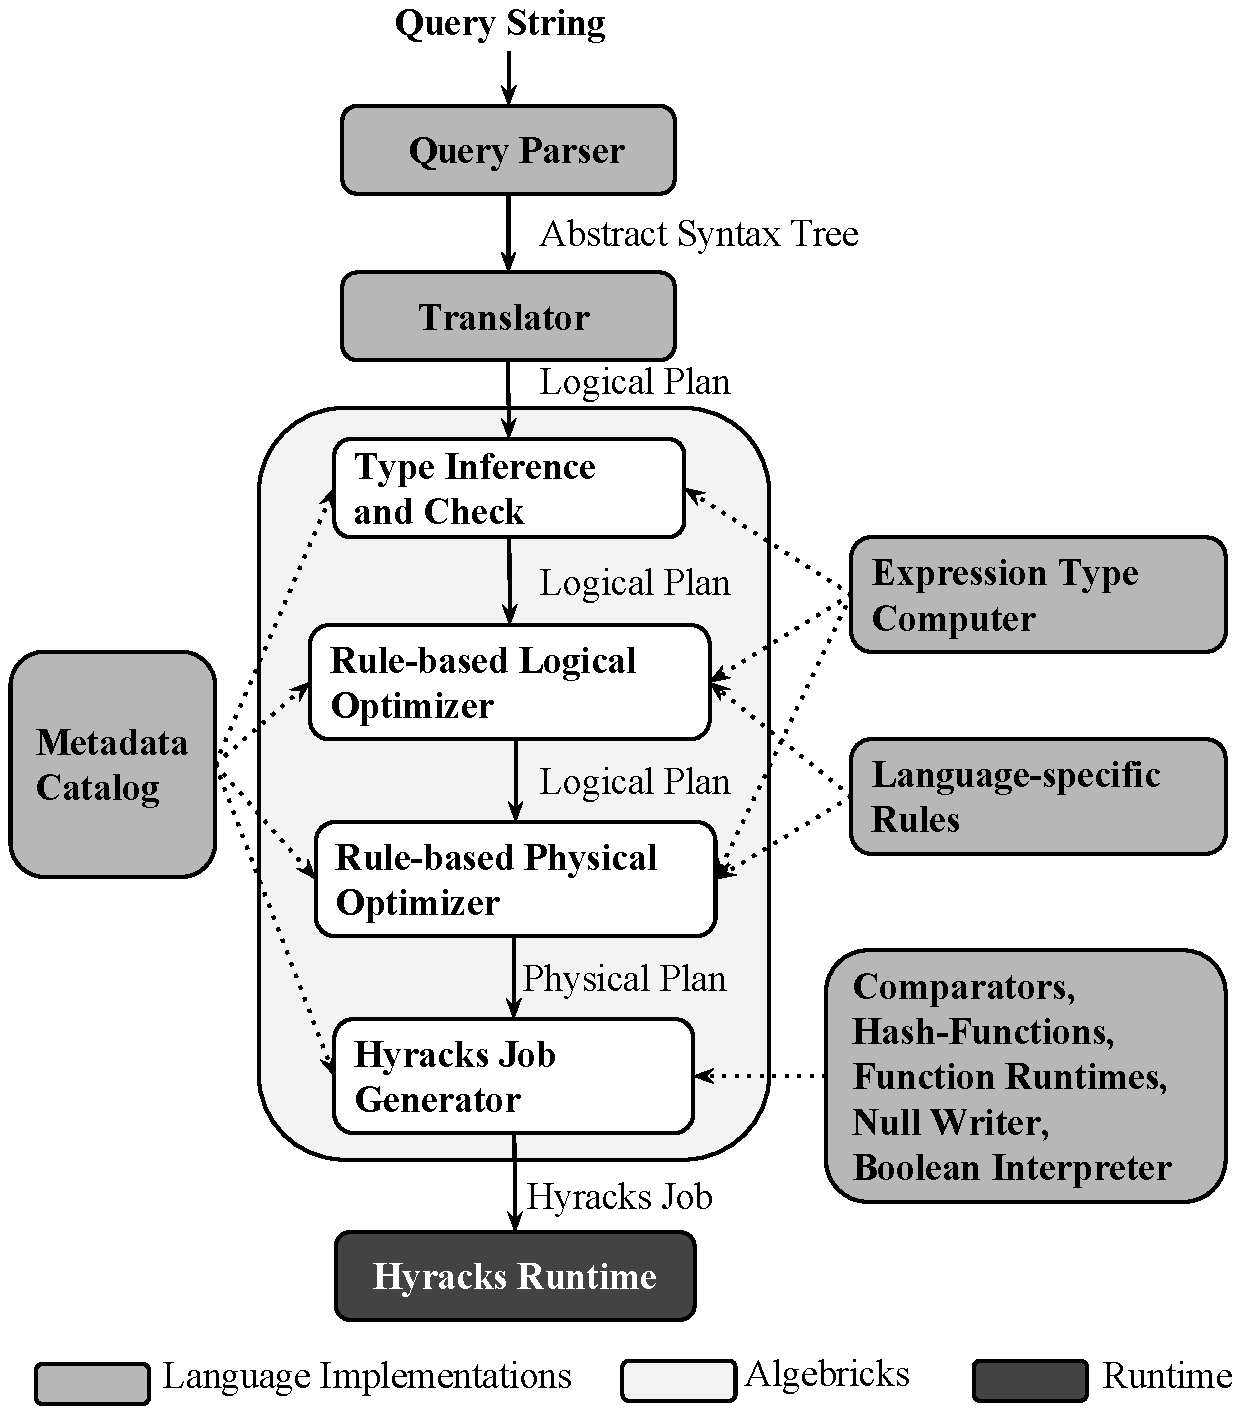
\includegraphics[width=5in]{images/compiler_flow}
  \vspace{-3ex}
  \caption{Flowchart of a typical Algebricks-based compiler.}
  \label{fig:flowchart}
\end{figure}

\textbf{Compilation Flow}. 
Figure~\ref{fig:flowchart} shows the typical sequence of compilation steps followed by a query processor built using Algebricks. 
An incoming query string is first lexically analyzed and parsed to construct an abstract syntax tree (AST).
This AST is then translated into 
the Algebricks logical plan, which is composed of logical operators (described in
Section~\ref{subsec:logoperators}) and serves as an intermediate representation to perform the next steps involved in query compilation. 
Type inference and checking is done over the initial logical plan, using a language-provided expression type computer which infers the type and checks type errors for each individual expression. 
The logical plan is then handed to the logical optimizer which rewrites it heuristically using logical rewrite rules. 
%The optimized logical plan is then translated to an Algebricks physical plan by selecting physical operators (described in
%section~\ref{subsec:phyoperators}) for every logical operation in the plan, by the physical optimizer. 
The physical optimizer translates the optimized logical plan to an Algebricks physical plan by selecting physical operators (described in
Section~\ref{subsec:phyoperators}) for every logical operation in the plan.
Both optimizers are rule-based and configured by selecting the set of rules to execute during the optimization phases.
The resulting physical plan is processed by the Hyracks Job Generator to produce a Hyracks job that is parallelized and evaluated by the Hyracks
execution engine.

\textbf{Rewriting Rules}. 
The query parser and translator (the first two stages in Figure~\ref{fig:flowchart} are query language specific and must be implemented by a query language developer. 
The next three stages (the optimizers and Hyracks job generator) are provided by the Algebricks library to be used by the developer. 
Algebricks also includes a library of language-agnostic rewrite rules that can be reused by the compiler developer. 
Additional language-specific rules are usually required in the optimization process, too. 
%VASSILIS Check
These need to be implemented by the developer by extending well-defined interfaces in the Algebricks library.
Note that a language-provided expression type computer should be called during certain rule applications to propagate updated types for the updated intermediate logical plans. 
The rewrite rule framework is described in Section~\ref{subsec:rewriter}.

\textbf{Metadata Catalog}. As shown in Figure~\ref{fig:flowchart}, the various phases of the query compilation process need access to information about the
environment in which the query is being compiled (usually described as catalog metadata). 
%The catalog contains metadata about data sources that are accessible in a query. 
The catalog is the authoritative source of logical properties of sources (such as schema,
integrity constraints, key information, etc.) and their physical properties (access methods, physical location, etc.) Algebricks
provides a Metadata Interface (Section~\ref{subsec:metadata}) that must be implemented by the compiler developer so that the various parts of the Algebricks
compiler can access relevant metadata information. 
%The Metadata Interface is described in Section~\ref{subsec:metadata}.

\textbf{Runtime Operations/Functions}. 
The Hyracks Job Generator maps physical operators selected by the Physical Optimizer to Hyracks runtime operators and connectors. 
In the process of this translation, the runtime operators need to be injected with data model-specific operations. 
The exact nature of the operation depends on the runtime operator being used. 
For example, the Sort operator  must be provided a comparator to compare two data model instances so that the input records can be sorted; the  Hash-Join operator needs a hash-function and a comparator to compute its result; the Select operator requires a boolean interpreter to interpret the result of its filtering condition expression; the Outer-Join operators need a null writer to generate null fields according to the language-defined data format. 
When using Algebricks, the language developer must provide families of operations (usually one family for each data type, for example, comparators and hash functions) that are needed for correct runtime Job construction.
Finally, the language developer must implement a mapping from function expressions to its own function runtime implementations (e.g., arithmetic functions, string functions, aggregate function, etc.) so that the data model agnostic runtime operators (e.g., select, assign, aggregate, etc.) can evaluate the data model-dependent functions.



\subsection{Metadata Interface}\label{subsec:metadata}

Every data-management system that accesses stored data or external data sources to process queries requires some form of metadata that describes locations of the stored files or external data sources and the various access paths available to get to the data bits. 
For example, relational databases use a catalog to store information (schema) about
the tables and indexes present in the database; such information is used by the query compiler when compiling query plans. 
Algebricks provides a Metadata Interface which must be implemented by the author of the host language so that the Algebricks compiler can access metadata information required during the compilation process. 
The goal of this interface is to allow Algebricks access to all relevant details about datasources while not constraining the host language to a specific representation of the metadata internally.
%
The Metadata Interface provides the following pieces of information to the compiler:

\begin{asparaitem}
\item \textbf{Data Source Metadata}. Stored collections of data or external data sources are both modeled as a Data Source in Algebricks. 
For example, in HiveQL, a table would be considered a Data Source while a dataset or an external data feed would be modeled as a Data Source in AsterixDB~\cite{ASTERIX,DBLP:conf/edbt/GroverC15}.
The Data Source interface enables Algebricks to get metadata about the data that it represents. 
Source metadata can be broadly classified as Logical Metadata and Physical Metadata. 
Logical Metadata about a Data Source includes the type information of the data it represents and other logical properties such as functional dependencies and integrity constraints (keys, etc.). 
Physical Metadata provides details of how the data is physically stored or obtained, specifically providing partitioning information and any local ordering present in the stored data.

\item \textbf{Access Path Binding}. The Metadata Interface in Algebricks also serves as a factory to create the runtime binding to connect the compiled Hyracks job to the ``last mile" (operators that are capable of reading the data from the stored location).

\item \textbf{Function Metadata}. Algebricks further uses the Metadata Interface to find Function Metadata to optimize function applications that appear in the plan being compiled.
\end{asparaitem}

\subsection{Logical Operators}\label{subsec:logoperators}

The logical operators in Algebricks draw inspiration from a variety of algebraic systems proposed for nested-relational models description
\cite{Jaeschke:1982:RAN:588111.588133,NST-Algebra} and for the processing of semi-structured data \cite{Papakonstantinou2003299,Jagadish:2002gu,Deutsch:2004:NFL:1316689.1316706}. 
Tuples in Algebricks are used as an abstraction that hold values.
Algebricks operators logically consume and produce collections of tuples. 
Tuples contain fields that are created and manipulated by the operators; 
field names are represented by names prepended with a \$ sign in the description that follows. 
Note that tuples as used in this section are not to be confused with tuples in the relational model, as Algebricks tuple field
values are allowed to be of arbitrary data types (not just scalar types like in the relational model). 
For example, in AsterixDB, an entire record (a composite data structure that contains name-value pairs) can be the value of a field in an Algebricks tuple and a concrete field type (i.e., open type in AQL~\cite{ASTERIX}) can even be determined at runtime.
\eat{\nick{I didn't fully understand the difference between tuples in Algebricks and in the relational model. Is it just that we allow nesting? Then we could say it is similar to nested relational datamodels or maybe to query languages with complex values. These are all well known concepts.}}

Operators may also contain references to scalar or aggregation functions wrapped inside a generic logical expression interface which exposes the used fields and allows for field name substitution. 
This allows Algebricks to rewrite the plan, while at runtime native functions are run against the data model of the implemented language.
A logical expression also has methods for computing logical constraints that can be inferred from that expression.
The constraints currently implemented are functional dependencies and equivalence classes.
They are used during rewriting, e.g. to reason about interesting orders and partitioning properties.
There are three implementations of the logical expression interface:
\eat{
\nick{The part about ILogicalExpression looks like it hasn't been integrated
it (probably my fault :-) It could have its own paragraph title, so it
stands out as a sub-topic. And rephrase the glue text to say more
clearly that we isolate everything related to scalars in these
ILogicalExpression instances.}
}

\begin{list}{\labelitemi}{\leftmargin=1em}\itemsep 0pt \parskip 0pt
\item {\em Constant} holds constant values.
\item {\em VariableReference} points to a logical variable (with a logical id) which is a column in a tuple.
\item {\em FunctionCall} holds a function identifier and references to argument expressions.
  It models all expressions which are not constants nor variables and it is the only kind of expression that is not a leaf in an expression tree.
\end{list}

{\em FunctionCall} is further refined by four implementations:

\begin{list}{\labelitemi}{\leftmargin=1em}\itemsep 0pt \parskip 0pt
\item {\em ScalarFunctionCall} is used for functions that compute their result by looking at only one tuple.

\item {\em AggregateFunctionCall} functions produce a result after iterating over a collection of tuples.
SQL aggregate functions belong here.
%fall in this category.

\item {\em StatefulFunctionCall} is similar to AggregateFunctionCall, but produces a result after each tuple, not only at the end. 
      Position variables in XQuery fall in this category: for every binding in a for-clause, they output the binding's index in the sequence.

\item {\em UnnestingFunctionCall} is given an input tuple and then can be called multiple times, each time returning a possibly different result, until a special value is returned. 
      Examples are the {\em range} function in Asterix which returns integer values from a specified range or the {\em collection} function in XQuery which returns nodes according to the arguments' available collection.
\end{list}

From a given function expression, a query language implementation can create the runtime artifact, i.e., an evaluator, 
which is capable of implementing its language-specific runtime semantics.
Evaluators run code specific to every language: in the case of Hivesterix (a HiveQL implementation on top of Algebricks; see Section~\ref{sec:hivesterix}), it runs the native Hive evaluators, which were not designed specifically for Algebricks. 
  Translation between logical function calls and evaluators is done at job generation time (Section~\ref{subsec:jobgen}). 
  This design has the advantage that it allows multiples ways of implementing the translation from logical to physical.
  In Hivesterix, this is done by having the function call expressions reference their evaluators.
  In AsterixDB, evaluators register themselves in a global map which is keyed on function identifiers.


\subsection{Physical Operators}\label{subsec:phyoperators}

While the logical operators described in Section~\ref{subsec:logoperators} capture the semantics of an Algebricks logical plan, physical operators are used to specify the exact algorithm to use for evaluating each operator. 
During the query rewrite process (described in Section~\ref{subsec:rewriter}) rules assign physical operators to each logical operator in the query plan, thus deciding the concrete algorithms to use in evaluating the query. 
Most logical operators in Algebricks map to a unique physical operator. 
However, Join and Group-By operators have multiple concrete implementations. Physically, joins can be performed using the Hybrid-Hash Join~\cite{DeWitt:1984:ITM:602259.602261} or the Nested-Loop Join algorithms. 
The Group-By operation can be performed using a pre-clustered implementation that assumes that its input is already clustered with respect to the 
grouping keys or by using a hash-based or sort-based Group-By algorithm that is capable of spilling to disk when the in-memory state exceeds available memory \cite{WenBCT13}.

In addition to physical operators corresponding to logical operators, Algebricks also provides physical operators to enforce order properties as well as partitioning properties of data distributed to individual operations during parallel evaluation of the query. 
Data distribution between operator partitions is expressed using an Exchange operator, motivated by~\cite{exchange}. 
\eat{\nick{It is true we use Exchange operators to enforce partition properties.
But Sort may also be used as an enforcer (for order properties), even
if the query semantics doesn't require sorting. In case we don't have
it somewhere else, we could add a short sentence saying we can
introduce enforcers for local properties (ordering and grouping).
 }
}
Currently, the data distribution strategies offered by Exchange operators in Algebricks are:

\begin{asparaitem}

\item {\em One-to-One Exchange}: This strategy is used for the local movement of data without redistribution of
data between partitions.

\item {\em Hash Exchange}: The Hash Exchange strategy hashes specified fields to determine how tuples are to be routed to the destination
partitions. This operator helps in partitioning data based on field values so that two tuples with the same partitioning field
values are routed to the same destination.

\item {\em Range Exchange}: The Range Exchange strategy uses a provided range vector to determine the destination partition to send a record to, based on the values of specified fields. 
The range vector maps disjoint ranges of values to target partitions. The value of the partitioning fields of each record are used to probe the range vector to decide the target partition. 
In addition to sending equal values to the same partition, range-based partitioning also sends close-by values to the same site. 
Such a distribution strategy is useful for performing a global sort in a parallel manner.

\item {\em Random Exchange}: Sometimes it is desirable to redistribute data to a set of partitions in a load-balanced manner, but without necessarily maintaining a value-based partitioning property. 
The Random Exchange Operator does exactly that by sending each record to a randomly determined partition.

\item {\em Broadcast Exchange}: The Broadcast Exchange strategy is used to make sure that the same data is delivered to every partition of the next operator. 
An example situation for the use of the Broadcast Exchange operator is while joining a small relation with a large partitioned relation. 
The small relation is broadcast to each machine where a partition of the large relation resides prior to performing a local join at each site.

\end{asparaitem}


%In addition to the data-exchange strategies listed above, 
Moreover, the Hash Exchange, Range Exchange, and Random Exchange strategies have a second variant each, namely, Hash-Merge Exchange, Range-Merge Exchange, and Random-Merge Exchange. A merge variant applies the same partitioning strategy as the non-merge variant, but uses a priority queue on the receiving side that merges all incoming streams so as to maintain a specified sort order that the data originally possessed before partitioning. 



\eat{
Table~\ref{tbl:phyoperators} summarizes the available
Physical Operators in Algebricks.

\begin{center}
\begin{table*}[ht]
{\small
\hfill{}
\begin{tabular}{ | l | l | p{3in} | }
\hline
Logical Operator & Physical Operator(s) & Description \\

\hline

\multirow{2}{*}{GroupBy Operator} & Presorted GroupBy & \\
\cline{2-3}
 & External Hash-Sort GroupBy & \\
\hline
\multirow{3}{*}{Join Operator} & Grace-Hash Join Operator & \\
\cline{2-3}
 & Hybrid-Hash Join & \\
\cline{2-3}
 & Nested-Loop Join & \\
\hline
\multirow{8}{*}{Exchange Operator} & One-to-One Exchange & \\
\cline{2-3}
 & Hash-Partition Exchange & \\
\cline{2-3}
 & Range-Partition Exchange & \\
\cline{2-3}
 & Random Exchange & \\
\cline{2-3}
 & Hash-Partition-Merge Exchange & \\
\cline{2-3}
 & Range-Partition-Merge Exchange & \\
\cline{2-3}
 & Random-Merge Exchange & \\
\cline{2-3}
 & Broadcast Exchange & \\
\hline
\end{tabular}
\caption{Algebricks Physical Operators}
\label{tbl:phyoperators}
}
\end{table*}
\end{center}
}

In Algebricks, the physical operator layer is extensible.
Compilers on top of Algebricks can register new physical operators by implementing the following interface:

\begin{java}
public interface IPhysicalOperator {
    public PhysicalRequirements requiredPropertiesForChildren(
        IPhysicalPropertiesVector requiredByParent);

    public void deliveredProperties(ILogicalOperator op,
        IOptimizationContext context);

    public void contributeRuntimeOperator(
        IHyracksJobBuilder builder,
        IOpSchema propagatedSchema, IOpSchema[] inputSchemas,
        IOpSchema outerPlanSchema);
}
\end{java}


The methods \codepiece{requiredPropertiesForChildren} and \codepiece{deliveredProperties} compute and propagate ordering, grouping and partitioning properties, close in spirit to SCOPE~\cite{ScopeJournal}.
These properties guarantee that the correct semantics of the operators are implemented, e.g., a Pre-Clustered Group-By will have its inputs partitioned by (a subset of) the group-by key and locally clustered on each partition, while allowing for optimizations, e.g., if the data partitioning already satisfies the requirements, no re-partitioning of the input is needed.
The \codepiece{contributeRuntimeOperator} method is essential in the job generation phase, discussed in Section~\ref{subsec:jobgen}.

In AsterixDB, we need physical operators for B-tree indexes, to enable efficient access to the native storage layer~\cite{storage}. 
Since they are AsterixDB specific, they cannot be part of the Algebricks library, so they are added as language specific operators for accessing its native storage layer~\cite{storage}.
%, including B-tree indexes, which are not part of the Algebricks library. 
The BTreeSearch physical operator's \codepiece{contributeRuntimeOperator} constructs a Hyracks B-Tree search runtime operator which is added to the job DAG together with an incoming edge from the Hyracks operator that produces the search intervals. 
BTreeSearch generally delivers a local ordering property on the key fields. For a primary index, the operator also delivers a hash-partitioning property of the key fields.
The operator generally requires its input (a stream of key intervals) be broadcast over the locations where the index is partitioned, but for primary indexes, the required property is hash-partitioning.

\eat{
If the output of the BTreeSearch operator is used by a join, \codepiece{requiredPropertiesForChildren} will generally have a broadcast requirement, but for an equality search on a primary index, this can be replaced by hash partitioning. 
Also, in the case of a primary index, the physical requirements contain a local order on the search keys so the B-tree search is more efficient.
}

\subsection{Rewriter}\label{subsec:rewriter}

The Algebricks optimizer uses Logical-to-Logical rewrite rules to create alternate logical formulations of the initial DAG.
Logical-to-Physical rewrite rules then generate a DAG of physical operators that specify the algorithms to use to evaluate the query.  
For example, a Join operator might be rewritten to a Hash-Join
physical operator. 
We expect that most language implementors using Algebricks will need a rewriting framework to perform additional useful data model-specific optimizations.
The Algebricks toolkit contains a rewriting framework that allows users to write their own rewrite rules, but it also comes with a number of ``out of the box'' rules that the user can choose to reuse for compiling their high-level language.
Examples of rules that apply for most languages include:

\begin{asparaitem}
\item {\bf Push Selects}: Rule for pushing filters lower in the plan to eliminate data that is not useful to the query.
\item {\bf Introducing Projects}: Rule to limit the width of intermediate tuples by eliminating values that are no longer needed
in the plan.
\item {\bf Query Decorrelation}: Rule to decorrelate nested queries to use joins when possible.
\end{asparaitem}

An example rule implemented in AsterixDB that is not of general applicability is one that uses ASTERIX metadata~\cite{ASTERIX} to determine if a field is present in the declared schema (i.e., if its presence is known a priori) in order to determine which field access method to use: field-access-by-index or field-access-by-name.

The rewriter uses the properties below, which, together with the graph of operators, dictate whether a rule is fired or not.
%Those properties include:

\begin{list}{\labelitemi}{\leftmargin=1em}\itemsep 0pt \parskip 0pt
\item {\bf Used/Produced Variables}. Operators schemas determine how projections and selections
are pushed and are needed by most rules that change the order of operators.

\item {\bf Functional Dependencies and Data Properties}. The process of rewriting into a physical DAG uses partitioning properties and local physical properties (grouping, ordering) of input data sources. 
Similar to SCOPE~\cite{ScopeJournal}, these are computed based on functional dependencies and variable equivalence classes.
Based on partitioning properties, Data Exchange operators~\cite{Dewitt:1990fk,journals/tkde/Graefe94} are introduced
to perform data redistribution between partitions.

\item {\bf Equivalence Classes}. The optimizer analyzes equivalence classes of variables.
%Variables within an equivalent class are equivalent to each other.
For example, after an equal inner join, a variable in the left-hand side join key
and its corresponding variable in the right-hand side join key are equivalent after the join operator. 
With the information of equivalent classes, functional dependencies and data properties are further propagated.
\end{list}

\subsection{Job Generation}\label{subsec:jobgen}

The job generation component outputs a Hyracks job implementing the Algebricks plan (Figure~\ref{fig:flowchart}).
The job is constructed by walking the plan and calling the \codepiece{contributeRuntimeOperator} method on the physical operators.
A physical operator can contribute either
\begin{inparaenum}[(a)]
  \item a full Hyracks operator,
  \item a micro-operator, which becomes part of a pipeline running inside one Hyracks operator,
  \item a connector, typically when the Algebricks operator is an exchange.
\end{inparaenum}
The Hyracks runtime for \codepiece{DataSourceScan} and 
\codepiece{WriteResult} operators are obtained through the Metadata Interface which also returns partitioning information needed to instantiate those operators. 
%In the case of sorting or join operators that need hash functions or comparators, they are picked based on the field types and set in the corresponding Hyracks operators.
%\nick{Is it still 1-to-1 between Algebricks plan and Hyracks job or could we generate multiple jobs to implement a plan?}
While the job generator currently only generates Hyracks jobs, its architecture conceptually supports other runtimes (e.g. Spark, Tez).
E.g., instead of generating Hyracks connectors, in Tez we would create ``edges" and in Spark ``partitioners", which are all similar concepts representing data movement from producers to consumers.


\section{Using Algebricks}
\label{sec:usage}

In this section we delve into the details of how three query processing systems --- Hivesterix (Hive-on-Hyracks), AsterixDB, and VXQuery --- use Algebricks to compile queries.

\subsection{Hivesterix}
\label{sec:hivesterix}
Hivesterix compiles HiveQL queries to run on the Hyracks platform.
For each HiveQL query, 
Hivesterix obtains the physical query plan from the Hive compiler
and turns that into an Algebricks logical plan for
Algebricks to produce a Hyracks job that calls
back to Hive's function evaluators at runtime.
Let us walk through a HiveQL example.
A simple HiveQL query shown below filters records from a TPC-H ``lineitem'' table to retain only those records which satisfy the filter predicate. 
Furthermore, the aggregated overall ``revenue" from selected records are returned. 
The ``lineitem'' table used in the query has the schema shown in Table~\ref{tbl:lineitemchema}. 

%\nick{The faded colored boxes for logical plans are not easy to read. Could we use something similar to the ones for the Hyracks jobs, even if just one box?}
\lstset{numbers=left, numberstyle=\tiny, stepnumber=1, numbersep=5pt}
\begin{center}
\scriptsize
\begin{lstlisting}
select sum(l_extendedprice*l_discount) as revenue
from lineitem
where l_shipdate >= '1994-01-01'
  and l_shipdate < '1995-01-01'
  and l_discount >= 0.05 and l_discount <= 0.07
  and l_quantity < 24;
\end{lstlisting}
\end{center}


Hivesterix translates this query into the Algebricks plan below. In the plan, ``algebricks-*" (e.g., algebricks-gte, algebricks-lte) is a function
that Algebricks can recognize during rewriting but will use a language-provided runtime implementation at evaluation time.

% TODO should this be vertical table instead of horizontal?
\begin{table*}
\tiny
\begin{center}
\begin{tabular}{|l|l|l|l|l|l|l|l|l|}
\hline
Column Name &  l\_orderkey & l\_partkey & l\_suppkey & l\_linenumber & l\_quantity & l\_extendedprice & l\_discount & l\_tax\\ 
\hline
Data Type & bigint & bigint & bigint & bigint & float & float & float & float\\
\hline
\hline
Column Name & l\_returnflag & l\_linestatus & l\_shipdate & l\_commitdate & l\_receiptdate &l\_shipinstruct & l\_shipmode & l\_comment\\
\hline
Data Type & string & string & string & string & float & float & string & string\\
\hline
\end{tabular}
\caption{Schema of the TPC-H lineitem table.}\label{tbl:lineitemchema}
\end{center}
\end{table*}


\eat{
\begin{table}[!ht]
\begin{center}
\begin{tabular}{|l|l|}
\hline
Column Name & Data Type \\
\hline
\hline
l\_orderkey & bigint \\
\hline
l\_partkey & bigint \\
\hline
l\_suppkey & bigint \\
\hline
l\_linenumber & bigint \\
\hline
l\_quantity & float \\
\hline
l\_extendedprice & float \\
\hline
l\_discount & float \\
\hline
l\_tax & float \\ 
\hline
l\_returnflag & string \\
\hline
l\_linestatus & string \\
\hline
l\_shipdate & string \\
\hline
l\_commitdate & string \\
\hline
l\_receiptdate & float \\
\hline
l\_shipinstruct & float \\
\hline
l\_shipmode & string \\
\hline
l\_comment & string \\
\hline
\end{tabular}
\caption{Schema of the TPC-H lineitem table.}\label{tbl:lineitemchema}
\end{center}
\end{table}
}

\begin{center}
\scriptsize
\begin{lstlisting}
WRITE_RESULT( $$revenue )
AGGREGATE( $$revenue:sum($$l_extendedprice*$$l_discount) )
SELECT( algebricks-and(
    algebricks-gte($$1_shipdate, '1994-01-01'),
    algebricks-lt($$1_shipdate, '1995-01-01'),
    algebricks-gte($$l_discount, 0.05),
    algebricks-lte($$l_discount, 0.07),
    algebricks-lt($$l_quantity, 24)) )
ASSIGN( $$l_shipdate, $$l_discount, $$l_extendedprice, 
    $$l_quantity:
    column_expr($l, "l_shipdate"),
    column_expr($l,"l_discount"),
    column_expr($l, "l_extendedprice"),
    column_expr($l,"l_quantity") )
UNNEST( $$l:dataset(lineitem) )
EMPTY_TUPLE_SOURCE
\end{lstlisting}
\end{center}

While reading Algebricks plans, it is important to note that the dataflow is assumed to flow from the bottom of the plan to the top. 
The ``unnest'' operator produces the tuple streams from rows in the ``lineitem'' table. 
The Metadata Interface (Section~\ref{subsec:metadata}) implemented in Hivesterix probes the Hive meta-store (the catalog database used by Hive-on-Hadoop) to get schema information about the table accessed by the query. 
As seen in Table~\ref{tbl:lineitemchema}, the ``lineitem'' table has sixteen columns. 
Note that the translator does not prune the source fields not used in the query.  
Algebricks includes the logic necessary to perform this pruning. 
Continuing on with the initial plan for the query, the translator creates an ``assign" operator to extract fields from input tuples and a ``select'' operator to represent the ``where'' clause in the query. 
Finally, the ``aggregate'' operator is used to perform the aggregate sum and a ``write'' operator is used to write the results to HDFS. 
%Readers will find this expression of the query reminiscent of relational algebra~\cite{relalgebra} expressions.

After the translated plan is constructed, Hivesterix proceeds to optimize the query.
The Hivesterix optimizer is populated with a total of 61 optimization rules out of which 4 rules are specific to Hivesterix and the rest are part of the common Algebricks framework. 
Figure~\ref{fig:hivestrix_hyracks_job} visualizes the finally generated Hyracks job from the optimizer.
The Algebricks rewrite rules have all the logic necessary to parallelize the query without the need for Hivesterix to provide any additional code. 


\begin{figure}[!ht]
\vspace{-.8ex}
\centering
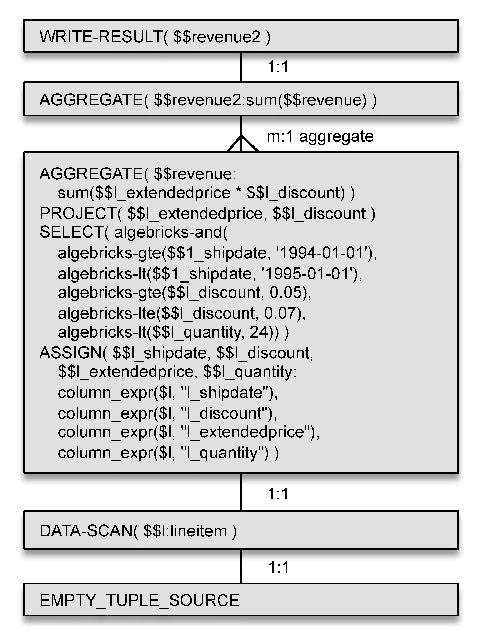
\includegraphics[width=0.70\columnwidth]{images/hivestrix_hyracks_job}
\vspace{-1ex}
\caption{Hivesterix Hyracks Job.}
\vspace{-.8ex}
\label{fig:hivestrix_hyracks_job}
\end{figure}


\eat{
\begin{center}
\scriptsize
\begin{lstlisting}
WRITE_RESULT( $$revenue2 )
ONE-TO-ONE EXCHANGE
AGGREGATE( $$revenue2:sum($$revenue) )
M-TO-ONE EXCHANGE
AGGREGATE( $$revenue:sum($$l_extendedprice*$$l_discount) )
ONE-TO-ONE
PROJECT( $$l_extendedprice, $$l_discount )
ONE-TO-ONE EXCHANGE
SELECT( algebricks-and(
    algebricks-gte($$1_shipdate, '1994-01-01'),
    algebricks-lt($$1_shipdate, '1995-01-01'),
    algebricks-gte($$l_discount, 0.05),
    algebricks-lte($$l_discount, 0.07),
    algebricks-lt($$l_quantity, 24)) )
ONE-TO-ONE EXCHANGE
ASSIGN( $$l_shipdate, $$l_discount, $$l_extendedprice,
    $$l_quantity:
    column_expr($l, "l_shipdate"),
    column_expr($l, "l_discount"),
    column_expr($l, "l_extendedprice"),
    column_expr($l, "l_quantity") )
ONE-TO-ONE EXCHANGE
DATA-SCAN( $$l:lineitem )
EMPTY_TUPLE_SOURCE
\end{lstlisting}
\end{center}
}

Note that most of the final Hyracks job looks similar to the original translated plan with the following differences:

\begin{list}{\labelitemi}{\leftmargin=1em}\itemsep 0pt \parskip 0pt
\item A project operator is injected into the plan to prune unnecessary columns.
\item An additional aggregate operator is injected to perform local aggregate in order to save the network bandwidth consumption, since the aggregation
function \textit{sum} is distributive.
\item An exchange operator with the associated data redistribution strategy has been introduced between every pair of operators. 
Operators below the lower aggregate operator use only one-to-one exchange operators.  
A m-to-one exchange is placed between the lower (local) aggregate and the higher (global) aggregate.
\end{list}



\subsection{Apache AsterixDB}

\eat{
\begin{itemize}
\item Very brief description of AsterixDB (one Paragraph)
\item Description of the datasets \& showing sample records 
\item Description of the query (in plain English)
\item Putting references to logical, optimized logical and physical plans
\item Describing the Hyracks job in details (broken into multiple phases): pushing selections down for each dataset, the intermediate partitioning step prior to the join, the HHJ step (AsterixDB uses HHJ for equi-joins), final record-construction step and results distribution)
\item Highlight and emphasize on the functions, rules and parts that fully reside in the AsterixDB code base (not part of the Algebricks) to clarify which parts are (re)-used from the Algebricks framework
\end{itemize}
}

Apache AsterixDB is a full-featured Big Data Management System for managing large quantities of semi-structured data. It is currently undergoing incubation at the Apache Software Foundation (ASF). 
AsterixDB's data model supports JSON-like data and adds more primitive and structured data types to JSON's data types.

As a slightly more complex example, consider the query below in the Asterix Query Language (AQL)~\cite{ASTERIX}.
This query performs a join between two natively stored data collections, ``GleambookMessages'' and ``GleambookUsers'',
that matches records from the two datasets on the ``author\_id'' and ``id'' fields respectively. Note that as allowed by the flexible AsterixDB data model,
``author\_id'' is not in the declared schema of ``GleambookMessages''
but ``id'' is part of the ``GleambookUsers'' schema.
Furthermore, we limit the results to contain users whose ``user\_since'' is within a time range and messages whose ``send\_time'' is within a specific time interval. Results are in the form of ADM (Asterix Data Model)~\cite{ASTERIX} records with two attributes, ``uname'' and ``message''. 

\begin{center}
\scriptsize
\begin{lstlisting}
for $message in dataset GleambookMessages
for $user in dataset GleambookUsers
where $message.author_id = $user.id 
  and $user.user_since >= datetime('2008-10-24T14:21:21')
  and $user.user_since < datetime('2008-10-25T14:21:21')
  and $message.send_time >=datetime('2011-02-24T20:01:48')
  and $message.send_time < datetime('2011-02-25T05:01:48')
return {"uname": $user.name, "message": $message.message}
\end{lstlisting}
\end{center}



\eat{
\begin{center}
\scriptsize
\begin{lstlisting}
{"message_id": int64("1"),
"author_id": int64("1"), 
"in_response_to": int64("33331"),
"sender_location": point("32.19,70.92"),
"send_time": datetime("2011-06-06T09:42:22"),
"message": "love samsung the screen is awesome"}

{"id": int64("1"),
"alias": "Chastity0001",
"name": "ChastityCarden",
"user_since": datetime("2010-05-07T19:13:33"),
"friend_ids":
 {{int64("2818"), int64("6982"), int64("13039")}}, 
"employment": [{"organization_name":"Streettax",
"start_date":date("2005-09-13")}]}
\end{lstlisting}
\end{center}
}

The AQL translator translates
the query to the following equivalent logical plan representation:

\lstset{numbers=left, numberstyle=\tiny, stepnumber=1, numbersep=5pt}
\begin{center}
\scriptsize
\begin{lstlisting}
DISTRIBUTE-RESULT( $$20 )
PROJECT( $$20 )
ASSIGN( $$20:open-record-constructor(
    "uname", field-access-by-name($$1, "name"),
    "message", field-access-by-name($$0, "message")) )
SELECT( algebricks-and(
    algebricks-eq(field-access-by-name($$0, "author_id"), 
        field-access-by-name($$1, "id")), 
    algebricks-ge(field-access-by-name($$1, "user_since"), 
        datetime("2008-10-24T14:21:21")), 
    algebricks-lt(field-access-by-name($$1, "user_since"), 
        datetime("2008-10-25T14:21:21")), 
    algebricks-ge(field-access-by-name($$0, "send_time"), 
        datetime("2011-02-24T20:01:48")), 
    algebricks-lt(field-access-by-name($$0, "send_time"), 
        datetime("2011-02-25T05:01:48"))) )
UNNEST( $$1:dataset("GleambookUsers") )
UNNEST( $$0:dataset("GleambookMessages") ) 
EMPTY_TUPLE_SOURCE
\end{lstlisting}
\end{center}

\begin{figure}[tb]
\vspace{-.8ex}
\centering
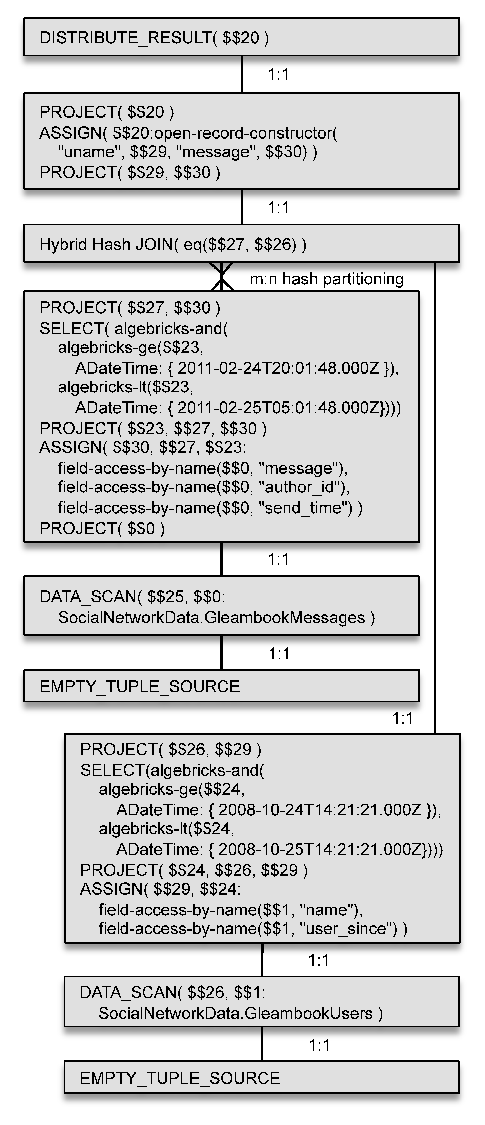
\includegraphics[width=0.5\columnwidth]{images/asterix_hyracks_job_renamed}
\vspace{-1ex}
\caption{AsterixDB Hyracks Job.}
\vspace{-.8ex}
\label{fig:asterix_hyracks_job}
\end{figure}

Then, the Algebricks optimizer transforms the initial logical plan into an optimized physical plan by applying logical and physical rewriting rules.
The optimizer utilizes 48 AsterixDB specific rules and 41 generic Algebricks rules. 
Figure~\ref{fig:asterix_hyracks_job} visualizes the generated Hyracks job for this example query.

Note that the final optimized Hyracks job has the following main differences from the original plan:

\begin{list}{\labelitemi}{\leftmargin=1em}\itemsep 0pt \parskip 0pt

\item A hybrid hash join operator is introduced to evaluate
the equality join condition.

\item The original select conditions are pushed into the two join branches.

\item Project operators are injected into the plan wherever necessary.

\item A hash partition exchange operator is enforced for the ``GleambookMessages'' branch to make sure data from this branch is partitioned by ``author\_id''.  Note that there is no re-partition exchange for the ``GleambookUsers'' branch because data from this branch has already been hash partitioned across the cluster according to the primary key ``id''.

\end{list}



\eat{
\begin{center}
\scriptsize
\begin{lstlisting}
DISTRIBUTE_RESULT( $$20 )
ONE_TO_ONE_EXCHANGE
PROJECT( $$20 )
ASSIGN( $$20:closed-record-constructor(
    "uname", $$29, "message", $$30) )
PROJECT( $$29, $$30 )
ONE_TO_ONE_EXCHANGE
Hybrid Hash JOIN( algebricks-eq($$27, $$26) )
{
  HASH_PARTITION_EXCHANGE( $$27 )
  PROJECT( $$27, $$30 )
  SELECT( algebricks-and(
      algebricks-ge($$23,
          ADateTime: { 2011-02-24T20:01:48.000Z }),
      algebricks-lt($$23, 
          ADateTime: { 2011-02-25T05:01:48.000Z })) )
  PROJECT( $$23, $$27, $$30 )
  ASSIGN( $$30, $$27, $$23:
      field-access-by-index($$0, 6), 
      field-access-by-index($$0, 2), 
      field-access-by-index($$0, 5) )
  PROJECT( $$0 )
  ONE_TO_ONE_EXCHANGE
  DATA_SCAN( $$25, $$0:demo.FacebookMessages )
  ONE_TO_ONE_EXCHANGE
  EMPTY_TUPLE_SOURCE
} {
  ONE_TO_ONE_EXCHANGE
  PROJECT( $$26, $$29 )
  SELECT( algebricks-and(
      algebricks-ge($$24,
          ADateTime: { 2008-10-24T14:21:21.000Z }), 
      algebricks-lt($$24, 
          ADateTime: { 2008-10-25T14:21:21.000Z })) )
  PROJECT( $$24, $$26, $$29 )
  ASSIGN( $$29, $$24:
      field-access-by-index($$1, 3), 
      field-access-by-index($$1, 5) )
  ONE_TO_ONE_EXCHANGE
  DATA_SCAN( $$26, $$1:demo.FacebookUsers )
  ONE_TO_ONE_EXCHANGE
  EMPTY_TUPLE_SOURCE
}
\end{lstlisting}
\end{center}
}


\subsection{Apache VXQuery}

\eat{
Highlights
\begin{itemize}

  \item path step optimizations
  \item xquery logic vs algebricks logic
  \item XML parser 
  \item query plan includes type information
\end{itemize}
}

Apache VXQuery is an XQuery processor built for handling large collections of XML data. 
It uses Algebricks and Hyracks to process XML by adding a binary representation of the XQuery Data Model (XDM), an XQuery parser, an XQuery optimizer, and the data model dependent expressions.
VXQuery is intended to implement the complete XQuery specification.

The example XQuery statement is based on weather data provided by the NOAA \cite{NOAA-GHCND:website}.
The query finds all precipitation ("PRCP") records for the "GHCND:USW00014771" station that occurred during 1999.
The precipitation readings are recorded in tenths of an inch.
After summing all readings, the result is divided by 10 to find the total precipitation for 1999 in inches.
The query (also included in our experiments as VQ2) is shown below followed by a sample XML weather record:

\lstset{numbers=left, numberstyle=\tiny, stepnumber=1, numbersep=5pt}
\begin{center}
\scriptsize
\begin{lstlisting}
fn:sum(
  for $r in collection("sensors")/dataCollection/data
  where $r/station eq "GHCND:USW00014771" 
    and $r/dataType eq "PRCP" 
    and year-from-dateTime(xs:dateTime(data($r/date))) 
        eq 1999
  return $r/value
) div 10
\end{lstlisting}
\end{center}

\lstset{numbers=left, numberstyle=\tiny, stepnumber=1, numbersep=5pt}
\begin{center}
\scriptsize
\begin{lstlisting}
<?xml version="1.0" encoding="UTF-8" standalone="yes"?>
<dataCollection pageCount="1" totalCount="3">
  <data>
    <date>1999-12-02T00:00:00.000</date>
    <dataType>PRCP</dataType>
    <station>GHCND:USW00014771</station>
    <value>0</value>
    <attributes>
      <attribute></attribute>
      <attribute></attribute>
      <attribute>a</attribute>
      <attribute></attribute>
    </attributes>
  </data>
  <data>
    <date>1999-12-02T00:00:00.000</date>
    <dataType>TMIN</dataType>
    <station>GHCND:USW00014771</station>
    <value>-6</value>
    <attributes>
      <attribute></attribute>
      <attribute></attribute>
      <attribute>0</attribute>
      <attribute></attribute>
    </attributes>
  </data>
</dataCollection>
\end{lstlisting}
\end{center}

Apache VXQuery begins by translating the XQuery statement into a logical query plan using the Algebricks logical operators.
The translator follows the XQuery specification and creates a correct Algebricks query plan with all the XQuery type checking expressions translated into the query plan.
The optimizer will use these expressions to type check the query plan.
%\yingyi{Prestion, is type checking done here?  It seems different
%from what we discussed.}.
%The translator takes a strict approach to building a logical query plan.
%The plan includes all the necessary type checking for data flowing through the query.

XQuery is a complex language with well-defined but complicated semantics for various parts of the language~\cite{XQuery-W3C-Formal-Semantics}.
Below we show the initial Algebricks logical plan generated by the VXQuery translator for the weather query.
Note that what appears as a simple path-step in XQuery (the / operator), is equivalent to a more complex expression that involves unnesting, sorting, duplicate-elimination, etc.
For example, lines 68-74 in the listing below represent "/dataCollection".
Please note that while we do not expect the reader to glean all the details of the plan shown, we wish to communicate the fact that Algebricks is capable of implementing the semantics of a complex query language like XQuery.

\newpage

%\definecolor{light-gray}{gray}{0.80}

\lstset{numbers=left, numberstyle=\tiny, stepnumber=1, numbersep=5pt}
\begin{center}
\scriptsize
\begin{lstlisting}
DISTRIBUTE-RESULT( $$59 )
UNNEST( $$59:iterate($$58) )
ASSIGN( $$58:divide(promote(<anyAtomicType?>, data($$56)), 
    promote(<anyAtomicType?>, data($$57))) )
ASSIGN( $$57:10 )
ASSIGN( $$56:sum(promote(<anyAtomicType*>, data($$55))) )
SUBPLAN {
  AGGREGATE( $$55:sequence($$54) )
  ASSIGN( $$54:sort-distinct-nodes-asc-or-atomics($$53) )
  SUBPLAN {
    AGGREGATE( $$53:sequence(child("value", 
        treat(<node*>, $$51))) )
    UNNEST( $$51:iterate($$49)
    NESTED-TUPLE-SOURCE
  }
  ASSIGN( $$49:treat(<item>, $$19) )
  SELECT( boolean($$48) )
  ASSIGN( $$48:and(boolean(data($$36)), 
      boolean(data($$47))) )
  ASSIGN( $$47:value-eq(promote(<anyAtomicType?>, 
      data($$45)), promote(<anyAtomicType?>,data($$46))) )
  ASSIGN( $$46:1999 )
  ASSIGN( $$45:year-from-dateTime(promote(<dateTime?>, 
      data($$44))) )
  ASSIGN( $$44:cast(<dateTime?>, $$43) )
  ASSIGN( $$43:data(treat(<item*>, $$42)) )
  ASSIGN( $$42:sort-distinct-nodes-asc-or-atomics($$41) )
  SUBPLAN {
    AGGREGATE( $$41:sequence(child("date", 
        treat(<node*>, $$39))) )
    UNNEST( $$39:iterate($$37) )
    NESTED-TUPLE-SOURCE
  }
  ASSIGN( $$37:treat(<item>, $$19) )
  ASSIGN( $$36:and(boolean(data($$27)), 
      boolean(data($$35))) )
  ASSIGN( $$35:value-eq(promote(<anyAtomicType?>, 
      data($$33)), promote(<anyAtomicType?>,data($$34))) )
  ASSIGN( $$34:"PRCP" )
  ASSIGN( $$33:sort-distinct-nodes-asc-or-atomics($$32))
  SUBPLAN {
    AGGREGATE( $$32:sequence(child("dataType", 
        treat(<node*>, $$30))) )
    UNNEST( $$30:iterate($$28) )
    NESTED-TUPLE-SOURCE
  }
  ASSIGN( $$28:treat(<item>, $$19) )
  ASSIGN( $$27:value-eq(promote(<anyAtomicType?>, 
      data($$25)),promote(<anyAtomicType?>,data($$26)) ) )
  ASSIGN( $$26:"GHCND:USW00014771" )
  ASSIGN( $$25:sort-distinct-nodes-asc-or-atomics($$24) )
  SUBPLAN {
    AGGREGATE( $$24:sequence(child("station", 
        treat(<node*>, $$22))) )
    UNNEST( $$22:iterate($$20) )
    NESTED-TUPLE-SOURCE
  }
  ASSIGN( $$20:treat(<item>, $$19) )
  UNNEST( $$19:iterate($$18) )
  ASSIGN( $$18:sort-distinct-nodes-asc-or-atomics($$17) )
  SUBPLAN {
    AGGREGATE( $$17:sequence(child("data", 
        treat(<node*>, $$15))) )
    UNNEST( $$15:iterate($$13) )
    ASSIGN( $$13:sort-distinct-nodes-asc-or-atomics($$12))
    NESTED-TUPLE-SOURCE
  }
  SUBPLAN {
    AGGREGATE( $$12:sequence(child("dataCollection", 
        treat(<node*>, $$10))) )
    UNNEST( $$10:iterate($$8) )
    ASSIGN( $$8:sort-distinct-nodes-asc-or-atomics($$7) )
    NESTED-TUPLE-SOURCE
  }
  SUBPLAN {
    AGGREGATE( $$7:sequence(child("root", 
        treat(<node*>, $$5))) )
    UNNEST( $$5:iterate($$3) )
    NESTED-TUPLE-SOURCE
  }
  ASSIGN( $$3:collection(promote(<string>, data($$2))) )
  ASSIGN( $$2:treat(<item>, $$1) )
  ASSIGN( $$1:"/sensors" )
  NESTED-TUPLE-SOURCE
}
EMPTY-TUPLE-SOURCE
\end{lstlisting}
\end{center}

After translating the plan, the Algebricks query optimization phase uses 22 Apache VXQuery rules and 30 generic Algebricks rules to create an optimized logical plan.
Apache VXQuery rules apply basic XQuery data type rules and path step expression optimizations to streamline the plan.
One of Algebricks' benefits to this plan is a more efficient way to calculate the aggregation.
Using Algebricks logical operators, the built-in rules enable efficient two-step aggregation across the cluster.
Further, the VXQuery query optimizer provides data specific details - enabling parallelization of the query plan.
Apache VXQuery achieves parallel execution simply by providing XQuery function properties to Algebricks. 
%Since XQuery's logical expressions use trinary logic, the Algebricks logic expressions are only used for optimizing when the XQuery expression is matched with a boolean effective value expresion ("boolean").
%The optimized query plan is show below:

In the job generation phase, the VXQuery Metadata Interface implementation finds how the non-fragmented XML documents are partitioned throughout a cluster.
Each machine has a unique set of XML documents residing in a directory specified by the query's fn:doc or fn:collection function.
While AsterixDB has a native storage option, Apache VXQuery scans external XML documents for each query.
The weather query uses the collection function to identify the ``sensors" directory on all nodes.
Using the plan and the metadata interface, Algebricks creates the Hyracks job shown in Figure \ref{fig:vxquery_hyracks_job}.

\begin{figure}[tb]
\vspace{-.8ex}
\centering
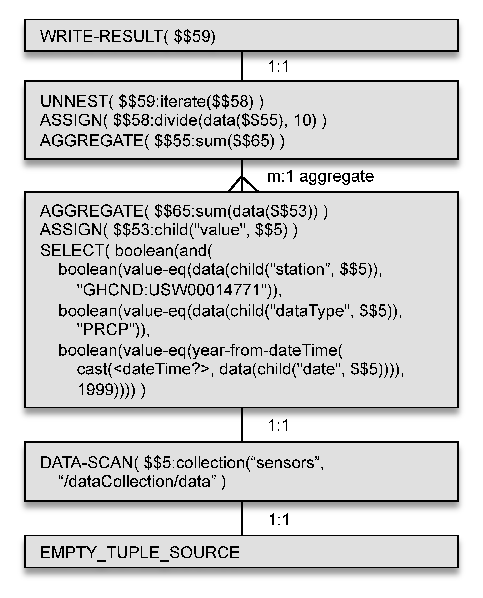
\includegraphics[width=0.50\columnwidth]{images/vxquery_hyracks_job}
\vspace{-1ex}
\caption{VXQuery Hyracks Job.}
\vspace{-.8ex}
\label{fig:vxquery_hyracks_job}
\end{figure}

\eat{
\begin{center}
\scriptsize
\begin{lstlisting}
DISTRIBUTE-RESULT ( $$59 )
ONE_TO_ONE_EXCHANGE
UNNEST( $$59:iterate($$58) )
ASSIGN( $$58:divide(data($$55), 10) )
AGGREGATE( $$55:sum($$65) )
RANDOM_MERGE_EXCHANGE
AGGREGATE( $$65:sum(data($$53)) )
ASSIGN( $$53:child("value", $$5) )
SELECT( boolean(and(
    boolean(value-eq(data(child("station", $$5)), 
        "GHCND:USW00014771")), 
    boolean(value-eq(data(child("dataType", $$5)), 
        "PRCP")), 
    boolean(value-eq(year-from-dateTime(cast(<dateTime?>, 
        data(child("date", $$5)))), 1999)))) )
ONE_TO_ONE_EXCHANGE
DATA-SCAN( $$5:collection("sensors", 
    "/dataCollection/data") )
ONE_TO_ONE_EXCHANGE
EMPTY-TUPLE-SOURCE
\end{lstlisting}
\end{center}
}

In the current implementation of VXQuery, we assume a collection of many (typically small) XML files. Nevertheless, Algebricks can also handle parallelization of queries over a single large document stored on a distributed storage system such as HDFS. We are currently implementing a parallel XML parser similar to \cite{oracle:xquery:website} to enable these use cases.
%Finally, Apache VXQuery can efficiently handle the query as long as each descendant tag node fits into the available memory.

\eat{
% Looks like this is covered inline for VXQuery
Note the following Apache VXQuery optimizations for the logical plan:

\begin{list}{\labelitemi}{\leftmargin=1em}\itemsep 0pt \parskip 0pt

\item The path step expression have been merged into the DATA-SCAN operator. As a result only the designated element is added to the data flow.

\item The aggregation is done using a local node sum and then a global sum from each node.

\item The SELECT operator's conditional expression has been inlined.

\end{list}
}


%The Metadata Interface specifies the XQuery parser, a SAX based XML parser, to read and translate the XML documents into XQuery Data Model (XDM) instances.
\eat{
The query demonstrates how Algebricks supports aggregation in multiple query languages.
In addition, Algebricks provides a framework to implement language specific optimizations: for example, XQuery has optimized the path step expression using Algebricks rewrite rules.
}

\section{Experimental Evaluation}\label{sec:experiments}

In this section, we demonstrate experimentally the parallel efficiency of Hivesterix, AsterixDB, and VXQuery. In addition to showing proof of their existence, these experiments aim to expose the direct benefits of using Algebricks in achieving good parallelization characteristics. We report performance for a representative set of queries for each system for different sizes of data and different numbers of nodes, with the goal of showing the scale-up and speed-up characteristics of each system.

\subsection{Hivesterix}
\noindent\textbf{Cluster}: We ran Hivesterix experiments on a 40-node cluster with a Gigabit Ethernet switch. 
Each node had a Quadcore Intel Xeon CPU E3-1230 V2 3.30GHz, 16GB of RAM, and 3TB RAID0 (3x1TB disks, linux software RAID). We compared Hivesterix and Hive-on-Hadoop (Hive-0.12.0). In the experiments,
the RAID0 disk on each node is used for the HDFS data directory
and the spilling workspace for query processing.
\noindent\textbf{Data}: For speedup experiments, we used TPC-H 250$\times$ (~250GB). For scaleup experiments, we used TPC-H 250$\times$,
500$\times$, 750$\times$, 1000$\times$ (~1TB) for 10, 20,
30, and 40 machines respectively.
\noindent\textbf{Configuration}: We ran eight partitions per machine.
\noindent\textbf{Queries}: We report three representative queries
from the TPC-H benchmark, a filter and aggregate query, a group-by query, and 
a join with group-by query, shown below.

\subsubsection*{HQ1: Filter + Aggregate Query (TPC-H Q14)}

\begin{lstlisting}
select sum(l_extendedprice*l_discount) as revenue
from lineitem
where l_shipdate >= '1994-01-01'
  and l_shipdate < '1995-01-01'
  and l_discount >= 0.05 and l_discount <= 0.07
  and l_quantity < 24;
\end{lstlisting}

\subsubsection*{HQ2: Group-by Query (TPC-H Q1)}

\begin{lstlisting}
select l_returnflag, l_linestatus, sum(l_quantity), 
  sum(l_extendedprice), 
  sum(l_extendedprice*(1-l_discount)),     
  sum(l_extendedprice*(1-l_discount)*(1+l_tax)), 
  avg(l_quantity), avg(l_extendedprice), avg(l_discount), 
  count(1) 
from lineitem 
where l_shipdate <= '1998-09-02' 
group by l_returnflag, l_linestatus 
order by l_returnflag, l_linestatus;
\end{lstlisting}

\subsubsection*{HQ3: Join + Group-By Query (TPC-H Q9)}

\begin{lstlisting}
select nation, o_year, sum(amount) as sum_profit
from (
  select n_name as nation, year(o_orderdate) as o_year, 
    l_extendedprice * (1 - l_discount) -  
    ps_supplycost * l_quantity as amount
  from orders o join (
    select l_extendedprice, l_discount, l_quantity, 
      l_orderkey, n_name, ps_supplycost 
    from part p join (
      select l_extendedprice, l_discount, l_quantity, 
        l_partkey, l_orderkey, n_name, ps_supplycost 
      from partsupp ps join (
        select l_suppkey, l_extendedprice, l_discount, 
          l_quantity, l_partkey, l_orderkey, n_name 
        from (
          select s_suppkey, n_name 
          from nation n join supplier s 
            on n.n_nationkey = s.s_nationkey
        ) s1 join lineitem l on s1.s_suppkey = l.l_suppkey
      ) l1 on ps.ps_suppkey = l1.l_suppkey 
          and ps.ps_partkey = l1.l_partkey
    ) l2 on p.p_name like '%green%' 
        and p.p_partkey = l2.l_partkey
  ) l3 on o.o_orderkey = l3.l_orderkey
) profit
group by nation, o_year
order by nation, o_year desc;
\end{lstlisting}

As indicated by Figures~\ref{fig:hivestrix_speed_up} and~\ref{fig:hivestrix_scale_up}, all queries show good speed-up and scale-up characteristics. All three benefit from scanning blocks of HDFS data in parallel. In HQ1 and HQ2, filtering is parallelized and aggregation is done in two phases, reducing the amount of data transferred across machines. HQ3 benefits from parallelizing joins across the cluster.
We have also executed TPC-H using Hive-on-Hadoop (Hive-0.12.0) and
a comparison with Hivesterix is shown in 
Figure~\ref{fig:hivestrix_hive}. (An interesting future exercise might include the new generation of "SQL on Hadoop" systems.)

\begin{figure}[!ht]
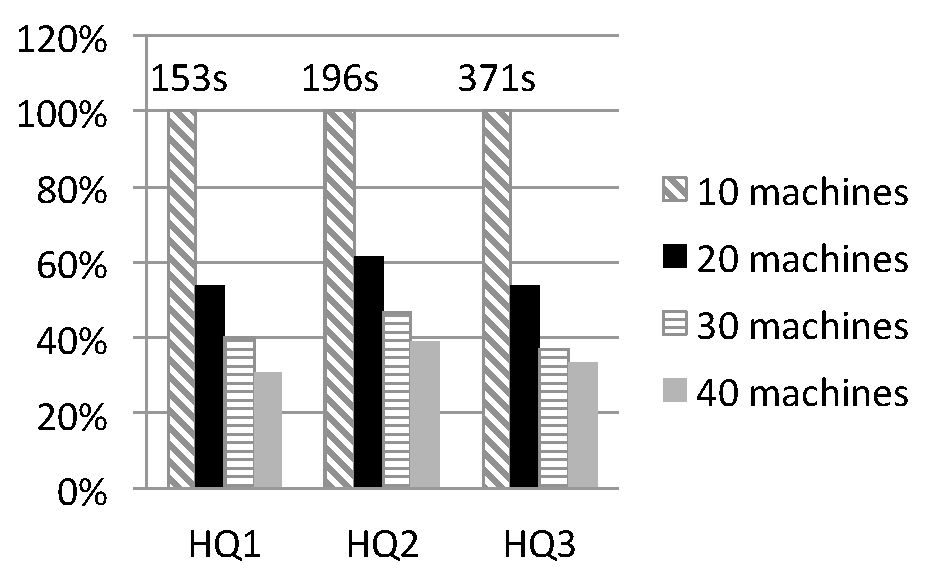
\includegraphics[width=\columnfigurewidth]{images/hivestrix_speed_up}
\centering
\vspace{-2ex}
\caption{Hivesterix cluster speed up (percentage of 10 machines).}
\label{fig:hivestrix_speed_up}
\end{figure}

\begin{figure}[!ht]
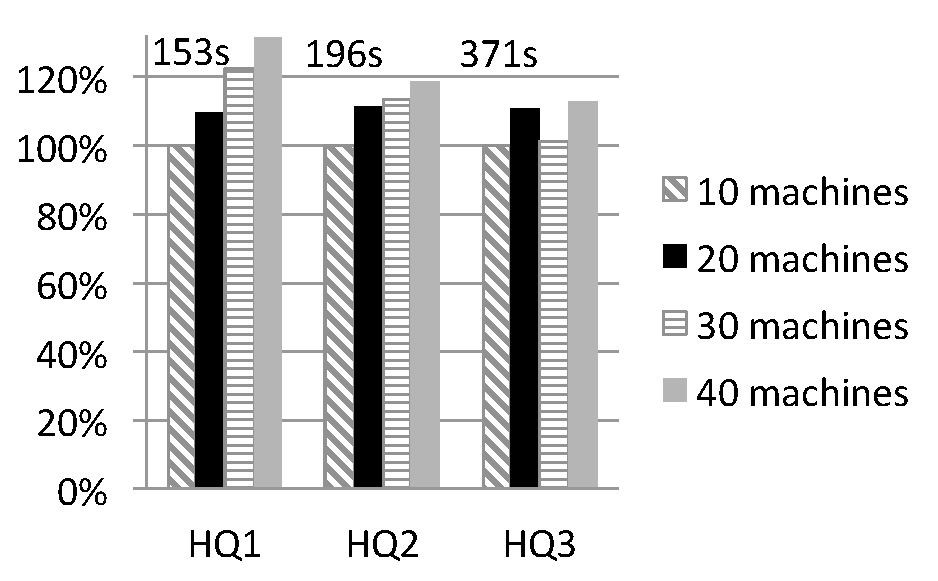
\includegraphics[width=\columnfigurewidth]{images/hivestrix_scale_up}
\centering
\vspace{-2ex}
\caption{Hivesterix cluster scale up (percentage of 10 machines).}
\label{fig:hivestrix_scale_up}
\end{figure}

\begin{figure}[!ht]
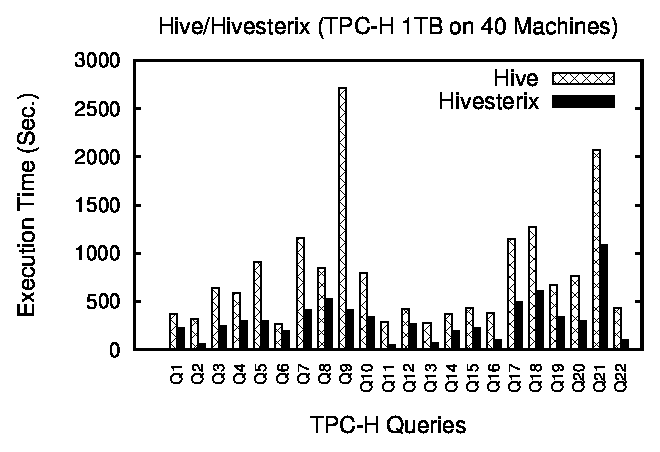
\includegraphics[width=\columnfigurewidth]{images/hivesterix}
\centering
\vspace{-1ex}
\caption{Hivesterix and Hive-on-Hadoop Comparison on TPC-H.}
\label{fig:hivestrix_hive}
\end{figure}


\subsection{Apache AsterixDB}

\eat{
\begin{itemize}
\item Asterix cluster description.
\item Show \& briefly describe each query.
\item Emphasize on the fact that the queries belong to different categories, and there is a huge difference in their running time (they do operations with naturally different costs and may exploit an index (as it exists in AsterixDB) which can change the data access path and performance considerably).
\item Present and explain Scale-up and Speed-up graphs separately.
\end{itemize}
}

\noindent\textbf{Cluster}: We ran the reported experiments on a 10-node IBM x3650 cluster with a Gigabit Ethernet switch. Each node had one Intel Xeon processor E5520 2.26GHz with four cores, 12GB of RAM, and four 300GB, 10K RPM hard disks. On each machine 3 disks were used for data. The other disk was used to store "system's data" (transaction logs and system logs).
\noindent\textbf{Data}: We used a synthetic data generator to create records for the collections related to these tests (``GleambookUsers'' etc.) For the speedup experiments, we generated 338GB of data, loaded on 9, 18 and 27 partitions. For the scaleup experiments, we generated 169GB, 338GB and 507GB of data for 9, 18 and 27 partitions respectively. A secondary index was constructed on the user\_since field of the GleambookUsers dataset.
%\yingyi{Pouria, can you please add the data description like that in the Hivesterix subsection?}
\noindent\textbf{Configuration}: We ran three partitions on each machine. 
We assigned a maximum of 6GB of memory to each node controller. 
The buffercache size for each node controller was set to be 1GB.
%\yingyi{Pouria, can you please add the configuration description like that in the Hivesterix subsection?}
\noindent\textbf{Queries}: We executed four representative AQL queries, as follows.

\subsubsection*{AQ1: Filter Query}

\begin{lstlisting}
for $t in dataset GleambookMessages
where $t.author_id < 0
return $t
\end{lstlisting}


\subsubsection*{AQ2: Filter Query Using Indexes}

\begin{lstlisting}
for $user in dataset GleambookUsers
where $user.user_since >= datetime('2005-08-16T15:52:14') 
and $user.user_since < datetime('2005-08-16T15:57:14') 
return $user
\end{lstlisting}



\subsubsection*{AQ3: Aggregate Query}

\begin{lstlisting}
avg(
  for $t in dataset ChirpMessages
  where $t.send_time >= datetime('2008-11-15T19:42:51')  
    and $t.send_time < datetime('2008-11-15T23:27:51')  
  return string-length($t.message_text)
)
\end{lstlisting}



\subsubsection*{AQ4: Join Query}

\begin{lstlisting}
for $message in dataset GleambookMessages
for $user in dataset GleambookUsers
where $message.author_id = $user.id 
  and $user.user_since >= datetime('2011-02-24T20:01:48')
  and $user.user_since < datetime('2011-02-25T05:01:48')
  and $message.send_time >=datetime('2008-10-24T14:21:21')
  and $message.send_time < datetime('2008-10-25T14:21:21')
return {
  "uname": $user.name,
  "message": $message.message
}
\end{lstlisting}


% Numbers can be found in the Google spread sheet.

\begin{figure}[tb]
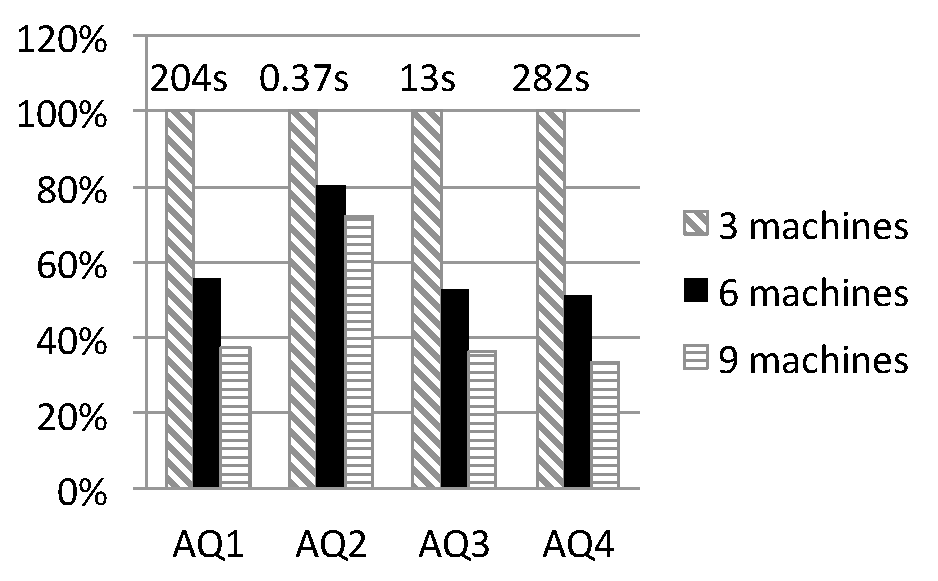
\includegraphics[width=\columnfigurewidth]{images/asterix_speed_up}
\centering
\vspace{-2ex}
\caption{AsterixDB cluster speed up (percentage of 3 machines).}
\label{fig:asterixdb_speed_up}
\end{figure}

\begin{figure}[tb]
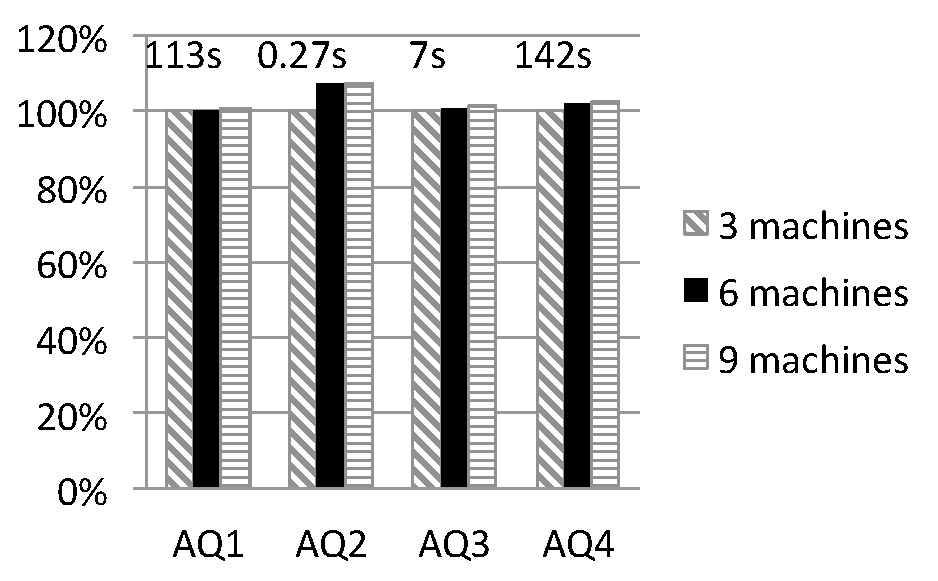
\includegraphics[width=\columnfigurewidth]{images/asterix_scale_up}
\centering
\vspace{-2ex}
\caption{AsterixDB cluster scale up (percentage of 3 machines).}
%\vspace{-3ex}
\label{fig:asterixdb_scale_up}
\end{figure}

Figure~\ref{fig:asterixdb_speed_up} and Figure~\ref{fig:asterixdb_scale_up} depict the parallel speedup and scaleup of the four AQL queries. AQ1 and AQ3 benefit from the same rules in Algebricks that helped HQ1 and HQ2 in Hivesterix. Scanning partitions and filtering is done in parallel on the different nodes of the cluster. In AQ3, the aggregation is performed in two phases to reduce network transfer. Join parallelism allows AQ4 to use the cluster effectively. AQ2 uses an index in AsterixDB to evaluate filters instead of scanning all the data. The index range scan is performed in parallel on the different partitions. Note that Algebricks includes facilities for utilizing indexes for query processing, but AsterixDB is currently the only system built on top of Algebricks that implements indexing at the storage level.
Detailed AsterixDB performance characteristics can be found in~\cite{ASTERIX}.



\subsection{Apache VXQuery}\label{sec:VXQuery}

\eat{
Highlights
\begin{itemize}

  \item XML parsing dominates query time 
  \item real weather data

\end{itemize}
}

\noindent \textbf{Cluster}: Experiments were run on a cluster whose nodes have two Dual-Core AMD Opteron(tm) processor 2212 HE CPUs, 8GB of RAM, and two 1TB hard drives. 
\noindent \textbf{Data}: We used NOAA's Global Historical Climatology Network (GHCN)-Daily dataset that includes daily summaries of climate recordings (e.g., high and low temperatures, wind speed, rainfall). 
The complete XML data definition can be found on NOAA's site \cite{NOAA-GHCND:website}. 
For the speed-up experiments, we used 57GB of weather  XML data partitioned over the number of machines (varied from 1 to 8) for each run.
The scale-up experiments were performed while keeping the amount of data per machine constant at 7.2GB and varying the number of machines from 1 to 8. 
%for each of the queries shown below.
\noindent \textbf{Configuration}: We ran four partitions per machine.
\noindent \textbf{Queries}: We used the following three XQuery queries:

\subsubsection*{VQ1: Filter Query}\label{query:VQ1}
% VQ1 represents VXQuery's benchmark query Q01
Query VQ1 filters the data to show all readings that report an extreme wind warning. 
Such warnings occur when the wind speed exceeds 110 mph. 
(The wind measurement unit, tenths of a meter per second, has been converted to miles per hour.)

\begin{lstlisting}
for $r in collection("sensors")/dataCollection/data
where $r/dataType eq "AWND"
  and xs:decimal(data($r/value)) gt 491.744
return $r
\end{lstlisting}


\subsubsection*{VQ2: Aggregate Query}\label{query:VQ2}
% VQ2 represents VXQuery's benchmark query Q02
Query VQ2 finds the annual precipitation for Syracuse, NY using the airport weather station (USW00014771) for 1999. 
The precipitation is reported in tenths of an inch. 

\begin{lstlisting}
sum(
  for $r in collection("sensors")/dataCollection/data
  where $r/station eq "GHCND:USW00014771" 
    and $r/dataType eq "PRCP" 
    and year-from-dateTime(xs:dateTime(data($r/date))) 
        eq 1999
  return $r/value
) div 10
\end{lstlisting}



\subsubsection*{VQ3: Join + Aggregate Query}\label{query:VQ3}
% VQ3 represents VXQuery's benchmark query Q05
Query VQ3 finds the lowest recorded temperature (TMIN) in the United States for 2001. 
This query includes nested loops which are commonly used in XQuery.
While XQuery does not have a join expression, these nested loops can be converted into a join operation using the Algebricks join operator.
Converting a nested loop into a more efficient join algorithm provides the expected performance improvement for Apache VXQuery.
%with a speed improvement over naive implementations. 


\begin{lstlisting}
min(
  for $s in 
      collection("stations")/stationCollection/station
  for $r in collection("sensors")/dataCollection/data
  where $s/id eq $r/station
    and (some $x in $s/locationLabels satisfies 
        ($x/type eq "CNTRY" and $x/id eq "FIPS:US"))
    and $r/dataType eq "TMIN" 
    and year-from-dateTime(xs:dateTime(data($r/date))) 
        eq 2001
  return $r/value
) div 10
\end{lstlisting}


% Numbers can be found in the Google spread sheet.

\begin{figure}[tb]
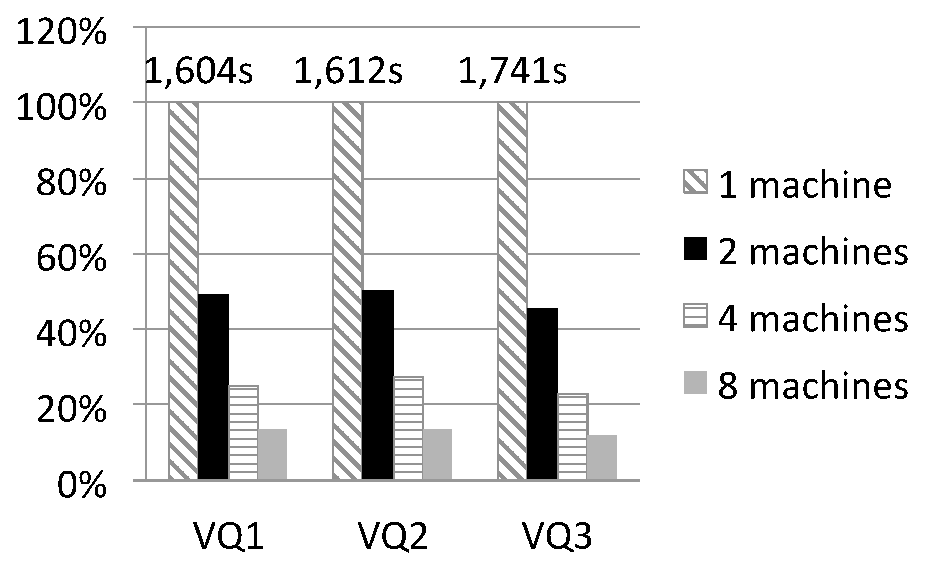
\includegraphics[width=\columnfigurewidth]{images/vxquery_speed_up}
\centering
\vspace{-2ex}
\caption{VXQuery cluster speed up (percentage of 1 machine).}
%\vspace{-1ex}
\label{fig:vxquery_speed_up}
\end{figure}

\begin{figure}[tb]
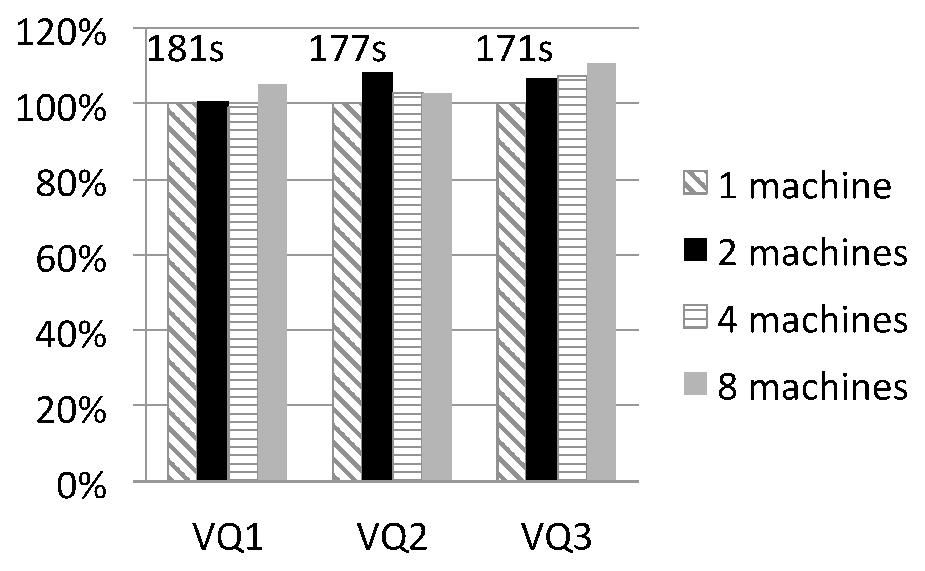
\includegraphics[width=\columnfigurewidth]{images/vxquery_scale_up}
\centering
\vspace{-2ex}
\caption{VXQuery cluster scale up (percentage of 1 machine).}
%\vspace{-1ex}
\label{fig:vxquery_scale_up}
\end{figure}

Figure~\ref{fig:vxquery_speed_up} and Figure~\ref{fig:vxquery_scale_up} show the parallel speedup and scaleup of Apache VXQuery. The optimizations implemented in Algebricks help VQ1, VQ2, and VQ3 to achieve good parallel performance by parallelizing scans, filters, aggregations, and joins.
More performance results for the current Apache VXQuery implementation on top of Algebricks can be found in \cite{Carman:2015}.

\section{Conclusion}

Algebricks has served as a useful tool to build not just the AsterixDB query compiler, but also query compilers for HiveQL and XQuery. Table~\ref{tbl:codemetrics} shows the lines of code, the number of rewrite rules, the number of logical operators, and the number of physical operators that were provided by Algebricks, and those that needed to be additionally implemented in AsterixDB, Hivesterix, and VXQuery. Algebricks provides about 50 rewrite rules, 39 logical operators, and 44 physical operators that are helpful for all three query processors. Additionally, AsterixDB required only 2 logical operators and 6 physical operators. These operators were AsterixDB specific and related to accessing indexes. The extensibility offered by Algebricks allowed the AsterixDB platform to implement these operators and plug them into the Algebricks framework. 61 rewrite rules were implemented in the AsterixDB platform to deal with rewrites specific to the Asterix data model. Hivesterix and VXQuery did not require any additional operators. Operators available in Algebricks were sufficient to implement the entire HiveQL and XQuery language compilers. Hivesterix and VXQuery required 4 and 29 rewrite rules, respectively, that were specific to the datamodel semantics of the two systems.


\begin{table}
\begin{center}
\begin{tabular}{|l|l|l|l|l|}
\hline
 & Algebricks & AsterixDB & Hivesterix & VXQuery \\
\hline
\hline
LOC & 42K & 40K & 3.4K & 12.8K \\
\hline
\# Rules & 50 & 61 & 4 & 29 \\
\hline
\# Logical Ops & 39 & 2 & 0 & 0 \\
\hline
\# Physical Ops & 44 & 6 & 0 & 0 \\
\hline
\end{tabular}
\caption{Code metrics as a proxy for the effort required to build query compilers using Algebricks}\label{tbl:codemetrics}
\end{center}
\end{table}

In the next chapter, we look more in detail at how Algebricks was used in implementing the query processing layer of AsterixDB.

\chapter{AsterixDB: Putting It All Together}
\label{ch:asterixdb}

\section{Overview}

Hyracks (Chapter~\ref{ch:hyracks}) and Algebricks (Chapter~\ref{ch:algebricks}) were developed in the context of the AsterixDB project, as mentioned in Chapter~\ref{ch:intro}. AsterixDB is a scalable Big-Data Management system built from the
ground up to ingest, manage, index, query, and analyze mass quantities semi-structured data~\cite{vision}. As a concluding case study, this chapter of the thesis describes
how Hyracks and Algebricks form the underpinnings of this Big-Data Management system. We begin by first providing an overview of AsterixDB's data definition capabilities (Section~\ref{ch:asterixdb:sec:ddl}) and its data manipulation capabilities (Section~\ref{ch:asterixdb:sec:dml}). In Section~\ref{ch:asterixdb:sec:sysarch}, we describe how Algebricks and Hyracks come together to form the bottom half of AsterixDB.

\section{Data Definition}
\label{ch:asterixdb:sec:ddl}

In this section we describe AsterixDB's data definition features.  We illustrate them by example through a scenario based on information about users and their messages from a hypothetical social network called Mugshot.com.

\subsection{Dataverses, Datatypes, and Datasets\label{ssec:dataverse}}

The top-level organizing concept in AsterixDB is the \emph{Dataverse}.
A Dataverse, short for "data universe", is a place (akin to a database in an RDBMS) within which one can create and manage the types, Datasets, functions, and other artifacts for a given application.
Initially, an AsterixDB instance contains no data other than the system catalogs, which live in a system-defined Dataverse (the Metadata Dataverse).
To store data in AsterixDB, one creates a Dataverse and then populates it with the desired Datatypes and Datasets.
A \emph{Datatype} specifies what its definer wants AsterixDB to know, a priori, about a kind of data that it will be asked to store.
A \emph{Dataset} is a stored collection of data instances of a Datatype, and one can define multiple Datasets of a given Datatype.
AsterixDB ensures that data inserted into a Dataset conforms to its specified type. 

Since AsterixDB targets semi-structured data, its data model provides the concept of \emph{open} (\emph{vs.~closed}) Datatypes.
When defining a type, the definer can use open Datatypes and tell AsterixDB as little or as much about their data up front as they wish.  
(The more AsterixDB knows about the potential residents of a Dataset, the less it needs to store in each individual data instance.)  
Instances of open Datatypes are allowed to have additional content, beyond what the type specifies, as long as they at least contain the information prescribed by the Datatype definition.  
Open types allow data to vary from one instance to another, leaving "wiggle room" for instance-level variations as well as for application evolution (in terms of what can be stored in the future). 
To restrict the objects in a Dataset to contain only what a Datatype says, with nothing extra in instances, one can opt to define a closed Datatype for that Dataset.
AsterixDB prevents users from storing objects with extra or illegally missing data in such a data set.
The closed, flat subset of ADM is thus relational.
Datatypes are open by default and closed only if their definition says so, the reason for this choice being that many Big Data analysts seem not to favor \emph{a priori} schema design and ADM's design targets semi-structured data.
To the best of our knowledge, this support for open and closed Datatypes is novel---we have not seen similarly flexible schema facilities in other data management systems, and it consistently garners very positive reactions when AsterixDB is presented to outside groups.

Shape-wise, ADM is a superset of JSON \cite{json}---ADM is what one gets by extending JSON with a larger set of Datatypes (e.g. datetime) and additional data modeling constructs (e.g. bags) drawn from object databases and then giving it a schema language.
We chose JSON for its self-describing nature, relative simplicity, and growing adoption in the Web world.
Note that, unlike AsterixDB, current JSON-based data platforms do not offer the option to define all (or part) of their data's schema.

%\begin{aql}[Data definition]{Dataverse and data types}{ddl:types}
\begin{ddl}[Dataverse and data types]{ddl:types}
drop dataverse TinySocial if exists;
create dataverse TinySocial;
use dataverse TinySocial;

create type EmploymentType as open {
    organization-name: string,
    start-date: date,
    end-date: date?
}

create type MugshotUserType as {
    id: int32,
    alias: string,
    name: string,
    user-since: datetime,
    address: {
        street: string,
        city: string,
        state: string,
        zip: string,
        country: string
    },
    friend-ids: {{ int32 }},
    employment: [EmploymentType]
}

create type MugshotMessageType as closed {
    message-id: int32,
    author-id: int32,
    timestamp: datetime,
    in-response-to: int32?,
    sender-location: point?,
    tags: {{ string }},
    message: string
}
\end{ddl}

We illustrate ADM by defining a Dataverse called \emph{TinySocial} to hold the Datatypes and Datasets for Mugshot.com.
The data definition statements in Data definition \ref{ddl:types} show how we can create the Dataverse and a set of ADM types to model Mugshot.com's users, their users' employment histories, and their messages. 
The first three lines tell AsterixDB to drop the old TinySocial Dataverse, if one exists, and to create a new Dataverse and make it the focus of the statements that follow. 
The first type creation statement creates a Datatype to hold information about one piece of a Mugshot user's employment history. 
It defines a record type with a mix of string and date data, much like a (flat) relational tuple.
Its first two fields are mandatory, with the last one (end-date) being optional as indicated by the "?" that follows it.
An optional field in ADM is like a nullable field in SQL -- it may be present or missing, but when present, its data type will conform to the Datatype's specification for it. Also, because EmploymentType is open, it is important to note that additional fields will be allowed at the instance level. 

\begin{table} [htbp]
\centering
\small
\begin{tabular}{|l|l|}
\hline %%%%%%%%%%%%%%%%%%%%%%%%%%%%%%%%%%%%%%%%%%%%%%%%%%%%%%%%
\textbf{Types}      & \textbf{functions}                     \\
\hline %%%%%%%%%%%%%%%%%%%%%%%%%%%%%%%%%%%%%%%%%%%%%%%%%%%%%%%%
string              & contains                               \\
                    & like                                   \\
                    & matches                                \\
                    & replace                                \\
                    & word-tokens                            \\
                    & edit-distance                          \\
                    & edit-distance-check                    \\
                    & edit-distance-contains                 \\
\hline %%%%%%%%%%%%%%%%%%%%%%%%%%%%%%%%%%%%%%%%%%%%%%%%%%%%%%%%
\emph{bag}          & similarity-jaccard                     \\
                    & similarity-jaccard-check               \\
\hline %%%%%%%%%%%%%%%%%%%%%%%%%%%%%%%%%%%%%%%%%%%%%%%%%%%%%%%%
date/time/datetime  & current-date/time/datetime             \\
interval            & interval-start-from-date/time/datetime \\
duration            & adjust-datetime-for-timezone           \\
day-time-duration   & adjust-time-for-timezone               \\
year-month-duration & subtract-date/time/datetime            \\
                    & interval-bin                           \\
                    & \emph{Allen's relations} on intervals  \\\hline %%%%%%%%%%%%%%%%%%%%%%%%%%%%%%%%%%%%%%%%%%%%%%%%%%%%%%%%
point               & spatial-distance                       \\
line                & spatial-area                           \\
rectangle           & spatial-intersect                      \\
circle              & spatial-cell                           \\
polygon             &                                        \\
\hline %%%%%%%%%%%%%%%%%%%%%%%%%%%%%%%%%%%%%%%%%%%%%%%%%%%%%%%%
\end{tabular}
\caption{Sample of advanced types and functions\label{tab:types}}
%\vspace{-0.1in}
\end{table}

The second create type statement creates a Datatype for Mugshot users.
MugshotUserType is also open since that is the default for AsterixDB Datatypes.
This second type highlights several additional features of ADM.
The address field illustrates one way that ADM is richer than the relational model; it holds a nested record containing the primary address of a user.
The friend-ids field shows another extension of ADM over the relational model and also over JSON.
This field holds a bag (unordered list) of integers -- presumably the Mugshot user ids for this user's friends.
Lastly for this type, its employment field is an ordered list of employment records, again a beyond-flat-relational structure.

The last create type statement in the example defines a Datatype to store the content of a Mugshot message.
In this case, since the type definition for Mugshot messages says \emph{closed}, the fields that it lists will be the only fields that instances of this type will be allowed to contain in Datasets of this type.
Also, among those fields, in-response-to and sender-location are optional, while the rest must be present in valid instances of the type.

Recall that AsterixDB aims to store and query not just Big Data, but Big \emph{Semi-structured} Data. 
Most of the fields in the create type statements above could be omitted, if desired, while changing only two things in terms of the example.  
One change would be the size of the data on disk. 
AsterixDB stores information about the fields defined \emph{a priori} as separate metadata; information about fields that are "just there" in instances of open Datatypes is stored within each instance.
A logical change would be that AsterixDB would be more flexible about the contents of records in the resulting Datasets, as it enforces only the specified details of the Datatype associated with a given Dataset.
The only fields that must currently be specified \emph{a priori} are the primary key fields. 

One other important feature of AsterixDB for managing today's Big Data is its built-in support for useful advanced primitive types and functions, specifically those related to space, time, and text.
Table \ref{tab:types} lists some of the advanced ADM primitive types as well as some of their corresponding AQL functions.
A complete list and more details can be found in the AsterixDB documentation \cite{docs}.

%spatial
%contructors (from coordinates or from string)
%accessors (get-x, get-y, get-points, get-center, get-radius)
%spatial-distance (between points)
%spatial-area (rectangle, circle, or polygon)
%spatial-intersect (2 spatial objects)
%spatial-cell

%constructors (from string)
%interval-from-date
%interval-from-time
%interval-from-datetime
%components (year/month/day/hour/minute/second/millisecond from data, time, datetime, duration)
%calendar-duration-from-datetime (normalize??)
%calendar-duration-from-date
%date-from-datetime, time-from-datetime
%date-from-unix-time-in-days, datetime-from-unix-time-in-ms, time-from-unix-time-in-ms
%get-interval-start, get-interval-end
%duration, year-month-duration, day-time-duration -> no functions?

\pagebreak
\subsection{Dataset and Index Creation}\label{ss:dataset}

Having defined our Datatypes, we can now proceed to create a pair of Datasets to store the actual data. 

\begin{ddl}[Datasets and indexes]{ddl:datasets}
create dataset MugshotUsers(MugshotUserType)
    primary key id;
create dataset MugshotMessages(MugshotMessageType)
    primary key message-id;

create index msUserSinceIdx 
    on MugshotUsers(user-since);
create index msTimestampIdx
    on MugshotMessages(timestamp);
create index msAuthorIdx
    on MugshotMessages(author-id) type btree;
create index msSenderLocIndex
    on MugshotMessages(sender-location) type rtree;
create index msMessageIdx
    on MugshotMessages(message) type keyword;
\end{ddl}

\eat{
use dataverse TinySocial;

load dataset MugshotUsers using localfs
(("path"="127.0.0.1:///Users/tillw/Documents/Papers/AsterixDB/703942dkdpdw/data/msu.adm.txt"),("format"="adm"));

load dataset MugshotMessages using localfs
(("path"="127.0.0.1:///Users/tillw/Documents/Papers/AsterixDB/703942dkdpdw/data/msm.adm.txt"),("format"="adm"));
}
\eat{
use dataverse TinySocial;

for $u in dataset MugshotUsers return $u;
for $m in dataset MugshotMessages return $m;
}

The two ADM DDL statements shown in Data definition \ref{ddl:datasets} will create Datasets to hold data in the TinySocial Dataverse.
The first creates a Dataset called MugshotUsers; 
this Dataset will store data conforming to MugshotUserType and has the id field as its primary key. 
The primary key is used by AsterixDB to uniquely identify instances for later lookup and for use in secondary indexes.
Each AsterixDB Dataset is stored (and indexed) as a B\textsuperscript{+}-tree keyed on primary key; secondary indexes point to indexed data by its primary key. 
Also, in an AsterixDB cluster, the primary key is used to hash-partition (shard) the Dataset across the cluster's nodes. 
The \emph{create dataset} statement for MugshotMessages is similar. 

%The last one illustrates an optional clause for providing useful hints to AsterixDB. 
%In this case, the hint tells AsterixDB that the dataset definer is anticipating that the TweetMessages dataset will contain roughly 100 objects; knowing this can help AsterixDB to more efficiently manage and query this dataset. 
%(AsterixDB does not yet gather and maintain data statistics; it will currently, abitrarily, assume a cardinality of one million objects per dataset in the absence of such an optional definition-time hint.)

The two \emph{create dataset} statements are followed by five more DDL statements, each requesting the creation of a secondary index on a field of one of the Datasets. 
The first two will index MugshotUsers and MugshotMessages on their user-since and timestamp fields. 
These indexes will be B\textsuperscript{+}-tree indexes, as their type is unspecified and \emph{btree} is the default. 
The other three show how to explicitly specify the desired index type. 
In addition to \emph{btree}, \emph{rtree} and inverted \emph{keyword} indexes are supported. 
Indexes can have composite keys, and more advanced text indexing is also available (\emph{ngram(k)}, where k is the gram length, for fuzzy searching).

\subsection{External Data}

So far we have explained how to specify Datatypes, Datasets, and indexes for AsterixDB to store and manage in its role as a full BDMS.  
AsterixDB also supports direct access to externally resident data.
Data does not need to be pre-loaded and handed to AsterixDB for storage and management just to be queried---avoiding the costly (and often infeasible) transfer or duplication of ``Big Data''.
The current AsterixDB system offers external data adaptors to access local files that reside on the Node Controller nodes of an AsterixDB cluster and to access data residing in HDFS. 
To illustrate, Data definition \ref{ddl:ext} shows the definition of an external Dataset based on a local file.  
In this case, the local file is a CSV version (Figure \ref{fig:csv-log}) of an Apache log file (Figure \ref{fig:apache-log}). 
When accessed at query time, CSV parsing of the data into ADM object instances will be driven by the type definition associated with the Dataset.

Once defined in this manner, an external Dataset can be accessed in a query just like any internal Dataset.
Unlike an internal Dataset, however, external Datasets in the current release of AsterixDB are limited to being read-only. More details about external datasets can be found in~\cite{DBLP:conf/cikm/AlamoudiGCB15}.

% \TODO{What happens if the type is open and % the CSV contains more fields than the type??}

\begin{figure*}
\lstinputlisting{data/apache.log.txt}
%\vspace*{\betweenfigureandcaption}
\caption{Apache HTTP server common log format\label{fig:apache-log}}
\end{figure*}

\begin{figure*}
\lstinputlisting{data/apache.csv.txt}
%\vspace*{\betweenfigureandcaption}
\caption{CSV version of web server log\label{fig:csv-log}}
\end{figure*}

\begin{ddl}[External data]{ddl:ext}
create type AccessLogType as closed {
    ip: string,
    time: string,
    user: string,
    verb: string,
    path: string,
    stat: int32,
    size: int32
}

create external dataset AccessLog(AccessLogType)
    using localfs
        (("path"="{hostname}://{path}"),
         ("format"="delimited-text"),
         ("delimiter"="|"));
\end{ddl}

% 127.0.0.1:///Users/tillw/Documents/Papers/AsterixDB/703942dkdpdw/data/apache.csv.txt

%    using hdfs (
%        ("hdfs"="{HDFS_URL}"), ("path"="{HDFS_PATH}"),
%        ("input-format"="text-input-format"),
%        ("format"="delimited-text"),
%        ("delimiter"="|"));
%\vspace{-0.1in}
\subsection{Data Feed Creation}\label{ss:feeds}

\emph{Data Feeds}~\cite{DBLP:conf/edbt/GroverC15} are a built-in mechanism that AsterixDB offers to allow new data to be continuously ingested into one or more Datasets from external sources, incrementally populating the Datasets and their associated indexes.
Feed support is provided because the need to persist and index "fast flowing" data is ubiquitous in the Big Data world, and it otherwise involves gluing together multiple systems. 
We feel that, just as current DBMSs were created to provide the commonly required functionality to support data-centric applications, a BDMS should provide support for continuous data ingestion and should be responsible for managing the performance and fault-tolerance of the ingestion pipeline.

An AsterixDB data feed ingests a continuous stream of data into a Dataset. 
User queries then work against the stored data, not on the incoming stream, just as if the Dataset's contents had arrived via loading or insertions. 
With this approach, the system does not require a separate notion of queryable streams (with their different semantics, etc.) distinct from its support for stored data sets.

Data definition \ref{ddl:feed} shows the declaration of a Data Feed and the connecting of it to a Dataset for storage. 
A socket-based feed adaptor is used, allowing data from outside to be pushed at AsterixDB via a TCP/IP socket where the adaptor will listen for data.

\begin{ddl}[Data feeds]{ddl:feed}
use dataverse TinySocial;

create feed socket_feed
    using socket_adaptor 
        (("sockets"="{address}:{port}"),
         ("addressType"="IP"),
         ("type-name"="MugshotMessageType"),
         ("format"="adm"));

connect feed socket_feed to dataset MugshotMessages;
\end{ddl}
\eat{
("sockets"="127.0.0.1:9009")
}

In addition to the \emph{socket\_adaptor} there are a few built-in adaptors included with AsterixDB.
To customize an existing adaptor it is also possible to apply a previously defined function (see Section \ref{ss:udfs}) to the output of the adaptor.
Finally, AsterixDB also provides a mechanism to add custom adaptors to the system.

Feeds that process external data, like the one above, are called \emph{Primary Feeds}. 
AsterixDB also supports \emph{Secondary Feeds} that are fed from other feeds.
Secondary Feeds can be used, just like Primary Feeds, to transform data and to feed Datasets or feed other feeds.
%Feed ingestion is a long running task and is bound to encounter hardware failure(s) as it runs on a cluster of machines. 
%Soft failures (runtime exceptions) may occur due to unexpected format or values of received data. 
%The degree of robustness associated with feed ingestion is configurable by means of associating an ingestion policy. For more details the reader is referred to \cite{AsterixFeeds}.
More about the user model for feeds, its extensibility, and its implementation and performance can be found in \cite{DBLP:conf/edbt/GroverC15}.

\subsection{User Defined Functions}\label{ss:udfs}

One final DDL feature that should be mentioned is  support for reusable \emph{user-defined functions} (UDFs), which are similar in nature to views in relational databases.
(AsterixDB's AQL UDFs are essentially views with parameters.)
As the definition of such a function requires an AQL function body, we will provide an example in Query \ref{q:function} in Section \ref{ch:asterixdb:sec:dml} and will provide more information about UDFs once we have introduced the reader to the basics of AQL.



\section{Data Manipulation}
\label{ch:asterixdb:sec:dml}

The query language for AsterixDB is AQL (Asterix Query Language).
Given the nature of ADM, we needed a language capable of dealing nicely with nesting and a lack of a priori schemas; we also wanted its semantics to be the same with and without schemas.
XQuery~\cite{xquery} had similar requirements from XML, so we chose to base AQL loosely on XQuery. 
ADM is simpler than XML, and XPath compatibility was irrelevant, so we jettisoned the ``XML cruft'' from XQuery---document order and identity, elements \emph{vs.} attributes, blurring of atomic and sequence values---keeping its core structure and approach to handling missing information.
We could have started over, but XQuery was co-designed by a diverse band of experienced language designers (SQL, functional programming, and XML experts) and we wanted to avoid revisiting many of the same issues and making mistakes that the W3C XQuery team had made, identified, and fixed in their years of work.
Starting from SQL would have been messier, syntactically and semantically, as ANSI SQL was designed for flat data---subqueries often have scalar-at-runtime-else-error semantics---and its treatment of nesting for its nested table feature is ugly and complex.
We wanted a much cleaner start for AQL.

AQL is an expression language; as such, the expression 1+1 is a valid AQL query that evaluates to 2.  
Most useful AQL queries are based on the FLWOR expression structure that AQL borrows from XQuery. 
FLWOR stands for \emph{for-let-where-order by-return}, naming the five most frequently used clauses of the full AQL query syntax. 
A \emph{for} clause provides an incremental binding of ADM instances in a sequence (e.g. a Dataset) to variables, while the \emph{let} clause provides a full binding of variables to entire intermediate result expressions.
Roughly speaking, the \emph{for} clause in AQL is like the \emph{FROM} clause in SQL, the \emph{return} clause in AQL is like the \emph{SELECT} clause in SQL (but goes at the end of a query), the \emph{let} clause in AQL is like SQL's \emph{WITH} clause, and the \emph{where} and \emph{order by} clauses in both languages are similar.
AQL also has \emph{group by} and \emph{limit} clauses, as we will see shortly. 

We will describe AQL by presenting a series of illustrative AQL queries based on our Mugshot.com schema. 
Most of the salient features of AQL will be presented, and of course more detail can be found in the online AsterixDB documentation \cite{docs}.

\begin{query}[All Datasets and indexes in the system]{q:metadata}
for $ds in dataset Metadata.Dataset return $ds;
for $ix in dataset Metadata.Index return $ix;
\end{query}

We begin our AQL tour with Query \ref{q:metadata}, which shows two queries that use the simplest (useful) \emph{for} and \emph{return} clauses and show how the keyword \emph{dataset} is used to access an AsterixDB Dataset in AQL.  
The queries each return the instances in a target Dataset, and each targets a Dataset in the Metadata Dataverse. 
The first one returns the set of all Datasets that have been defined so far, and the second one returns the set of all known indexes. 
These queries highlight the useful fact that AsterixDB ``eats its own dog food'' with respect to system catalogs---AsterixDB metadata is AsterixDB data, so (unlike Hive, for example) AsterixDB catalogs are stored in the system itself, as is also true in most RDBMSs.

\eat{ % "old version"
\begin{query}[Find a record]{q:lookup}
for $user in dataset MugshotUsers
where $user.id = 8
return $user;
\end{query}

Query \ref{q:lookup} illustrates an AQL where clause. This query's \emph{for} clause conceptually iterates over all records in the Dataset \emph{MugshotUsers}, binding each to the variable \emph{\$user}, returning ADM records whose \emph{id} field contains the value 8.
(Of course, as \emph{id} is the key field of the Dataset \emph{MugshotUsers}, the query's actual evaluation will be more efficient, utilizing the Dataset's primary index under the covers.) 
}

\begin{query}[Datetime range scan]{q:range-scan}
for $user in dataset MugshotUsers
where $user.user-since >= datetime('2010-07-22T00:00:00')
  and $user.user-since <= datetime('2012-07-29T23:59:59')
return $user;
\end{query}

Query \ref{q:range-scan} illustrates an AQL where clause. This query's \emph{for} clause conceptually iterates over all records in the Dataset \emph{MugshotUsers}, binding each to the variable \emph{\$user}, returning the ADM records for users  that joined mugshot.com from July 22, 2010 to July 29, 2012.
(Of course,  the query's actual evaluation may be more efficient, e.g., using an index on \emph{user-since} under the covers.) 

\begin{query}[Equijoin]{q:equijoin}
for $user in dataset MugshotUsers
for $message in dataset MugshotMessages
where $message.author-id = $user.id
  and $user.user-since >= datetime('2010-07-22T00:00:00')
  and $user.user-since <= datetime('2012-07-29T23:59:59')
return {
  "uname" : $user.name,
  "message" : $message.message
};
\end{query}

Query \ref{q:equijoin} shows a first example where new records are being synthesized by a query.
It first selects user records like Query \ref{q:range-scan}, but then it also selects matching message records whose \emph{author-id} is equal to the user's \emph{id}---an equijoin expressed in AQL.
For each match, it creates a new ADM record containing two fields, \emph{uname} and \emph{message}, that will contain the user’s name and the message text, respectively, for that user/message pair. 
Note that the query returns a sequence of flat records, i.e., it repeats the user name with every message. Also, as the match predicate is only true when a match exists, users without matching messages and messages without matching users are not returned.

\begin{query}[Nested left outer-join]{q:outer-join}
for $user in dataset MugshotUsers
where $user.user-since >= datetime('2010-07-22T00:00:00')
  and $user.user-since <= datetime('2012-07-29T23:59:59')
return {
  "uname" : $user.name,
  "messages" :
    for $message in dataset MugshotMessages
    where $message.author-id = $user.id
    return $message.message
};
\end{query}

Query \ref{q:outer-join} shows a more natural way to match users and messages in AQL.
Users of interest are targeted by the first \emph{for} and \emph{where} clause, and a nested \emph{FLWOR} expression synthesizes a bag of matching messages for each user.
In contrast to Query \ref{q:equijoin}, the result will include users who have not yet sent any messages, and the result will be a set of nested ADM records, one per user, with each user's messages listed ``inside'' their user record.
This is the equivalent of a SQL left outer join in AQL, but with a more natural result shape since ADM permits nesting (unlike the relational model).

\begin{query}[Spatial join]{q:spatial-join}
for $t in dataset MugshotMessages
return {
  "message" : $t.message,
  "nearby-messages":
    for $t2 in dataset MugshotMessages
    where spatial-distance($t.sender-location,
                           $t2.sender-location) <= 1
    return { "msgtxt" : $t2.message }
};
\end{query}

Query \ref{q:spatial-join} shows another ``join'' example, one that illustrates the use of AsterixDB's spatial data support. 
This query goes through the set of all Mugshot messages and, for each one, uses a nested query to pair it with a bag of messages sent from nearby locations.

\begin{query}[Fuzzy selection]{q:fuzzy-string-join}
set simfunction "edit-distance";
set simthreshold "3";

for $msu in dataset MugshotUsers
for $msm in dataset MugshotMessages
where $msu.id = $msm.author-id
  and (some $word in word-tokens($msm.message)
       satisfies $word ~= "tonight")
return {
  "name" : $msu.name,
  "message" : $msm.message
};
\end{query}

Query \ref{q:fuzzy-string-join} illustrates some of AsterixDB's \emph{fuzzy} matching capabilities.
This query returns the sending user name along with a message if one of the words in a tokenization of the message fuzzily matches (^~=^) "tonight".
\emph{Fuzzy} in this case means that the edit-distance is less than or equal to 3, e.g., a message that contains the word "tonite" would also be returned. 
The \emph{set} statements in the query's prologue are used to specify the desired fuzzy matching semantics;  a functional syntax for fuzzy matching is also available to specify the matching semantics within the matching predicate itself (which is needed if a query requires multiple fuzzy match predicates, each with different match semantics).

\begin{query}[Existential quantification]{q:existential}
for $msu in dataset MugshotUsers
where (some $e in $msu.employment 
       satisfies is-null($e.end-date)
         and $e.job-kind = "part-time")
return $msu;
\end{query}

Query \ref{q:existential} illustrates two more advanced aspects of AQL, namely existential quantification and the use of an open field (one that's not part of the type definition for the data in question).
This example query uses existential quantification in its \emph{where} clause to find users who have a current employment record (i.e., one with a null \emph{end-date}) that has a job-kind field whose value is \emph{"part-time"}.
(Note that \emph{job-kind} is not declared to be a field of \emph{EmploymentType}.)

\begin{query}[Universal quantification and function definition]{q:function}
create function unemployed() {
  for $msu in dataset MugshotUsers
  where (every $e in $msu.employment 
         satisfies not(is-null($e.end-date)))
  return {
    "name" : $msu.name,
    "address" : $msu.address
  }
};
\end{query}

\begin{query}[Function use]{q:call}
for $un in unemployed()
where $un.address.zip = "98765"
return $un
\end{query}

Query \ref{q:function} defines a function (similar to a view in SQL) that returns the name and address of unemployed users.
It tests for unemployed users by seeing that all their employments have ended.
Query \ref{q:call} then uses this function and selects all unemployed users in the ZIP code 98765. Such a function can be written by an experienced user (one with a taste for universal quantifiers) and then used by a novice user (one with more normal tastes).

\begin{query}[Simple aggregation]{q:agg}
avg(
  for $m in dataset MugshotMessages 
  where $m.timestamp >= datetime("2014-01-01T00:00:00")
    and $m.timestamp <  datetime("2014-04-01T00:00:00")
  return string-length($m.message)
)
\end{query}

Like any reasonably expressive query language, AQL includes support for aggregation. Query \ref{q:agg} is a first example of an AQL aggregate query, computing the average message length during a time interval of interest. 
AQL aggregates include \emph{count}, \emph{min}, \emph{max}, \emph{avg}, and \emph{sum} as well as \emph{sql-count}, \emph{sql-min}, \emph{sql-max}, \emph{sql-avg}, and \emph{sql-sum}. AQL's own aggregates have what we consider to be ``proper'' semantics regarding null values; e.g., the average of a set of values is null (unknown) if any of the values encountered is null. 
AQL also offers a set of aggregate functions with SQL's ``best guess'' null handling semantics, wherein the average of a set of values with nulls is the sum of the non-null values divided by the number of non-null values.

\eat{
\begin{query}[Grouping and aggregation]{q:gagg}
for $msg in dataset MugshotMessages
group by $aid := $msg.author-id with $msg
return {
  "author" : $aid,
  "no messages" : count($msg)
};
\end{query}
}

\begin{query}[Grouping with sorting and limits]{q:sort}
for $msg in dataset MugshotMessages
where $msg.timestamp >= datetime("2014-02-20T00:00:00")
  and $msg.timestamp <  datetime("2014-02-21T00:00:00")
group by $aid := $msg.author-id with $msg
let $cnt := count($msg)
order by $cnt desc
limit 3
return {
  "author" : $aid,
  "no messages" : $cnt
};
\end{query}

AQL supports grouped aggregation as well and also provides the machinery to get the `top'' results.
Query \ref{q:sort} illustrates how the \emph{group by}, \emph{order by}, and \emph{limit} clauses can be used to group and count messages by their sender and to report the results only for the three chattiest Mugshot.com users.
The \emph{group by} construct in AQL is designed to perform grouping on the specified keys (\$msg.author-id in Query~\ref{q:sort}), and implicitly create collections of the variable refernced in the \emph{with} clause. Logically, after the \emph{group by} clause, the variables present in the query until then go out of scope. The only values that are present after grouping are the keys and the collection created by the \emph{with} clause. In order to be able to access the keys, each key can be optionally bound to a variable that is in scope after grouping. In Query~\ref{q:sort}, \$aid holds the value of author-id for each group. The \emph{with} variable is re-bound after grouping to the collection.

\begin{query}[Active users]{q:active}
let $end := current-datetime()
let $start := $end - duration("P30D")
for $user in dataset MugshotUsers
where some $logrecord in dataset AccessLog
  satisfies $user.alias = $logrecord.user
  and datetime($logrecord.time) >= $start 
  and datetime($logrecord.time) <= $end
group by $country := $user.address.country with $user
return {
  "country" : $country,
  "active users" : count($user)
}
\end{query}

Query \ref{q:active} identifies all \emph{active} users and then counts them grouped by country.
The query considers users that had activity in the last 30 days to be active.
Activity data is taken from the web server logs that are exposed as an external dataset (see Figure \ref{fig:csv-log}).
This example also shows the use of datetime arithmetic in AQL.

\begin{query}[Left outer fuzzy join]{q:fuzzy-join}
set simfunction "jaccard";
set simthreshold "0.3";

for $msg in dataset MugshotMessages
let $msgsSimilarTags := (
  for $m2 in dataset MugshotMessages
    where  $m2.tags ~= $msg.tags
      and $m2.message-id != $msg.message-id
    return $m2.message
  )
where count($msgsSimilarTags) > 0
return {
  "message" : $msg.message,
  "similarly tagged" : $msgsSimilarTags    
};
\end{query}

Last but not least, Query \ref{q:fuzzy-join} closes out our tour of AQL's query power by showing how one can express fuzzy joins in AQL. 
This example analyzes Mugshot.com's messages by finding, for each message where there are one or more counterparts with similar tags, the similarly tagged messages. 
Here similarity means Jaccard similarity of 0.3 (messages with more than 30\% of the same tags). 
Under the covers AsterixDB has built-in support for both ad hoc parallel fuzzy joins as well as indexed fuzzy joins.

\begin{update}[Simple insert]{upd:insert}
insert into dataset MugshotUsers
(
  { 
    "id":11, 
    "alias":"John", 
    "name":"JohnDoe", 
    "address":{ 
      "street":"789 Jane St", 
      "city":"San Harry", 
      "zip":"98767", 
      "state":"CA", 
      "country":"USA" 
    }, 
    "user-since":datetime("2010-08-15T08:10:00"), 
    "friend-ids":{{ 5, 9, 11 }}, 
    "employment":[{ 
        "organization-name":"Kongreen", 
        "start-date":date("2012-06-05")
    }]
  }
);
\end{update}


\begin{update}[Simple delete]{upd:delete}
delete $user from dataset MugshotUsers 
where $user.id = 11;
\end{update}

Data can enter AsterixDB via loading, feeds, or insertion. AQL's support for \emph{insert} operations is illustrated in Update \ref{upd:insert}; its corresponding support for doing \emph{delete} operations is shown in Update \ref{upd:delete}. 
The data to be inserted is specified as any valid AQL expression; in this case the expression is a new record whose content is known a priori. 
Delete operations' \emph{where} clauses can involve any valid AQL boolean expression. 
Currently the AsterixDB answer for modifying data in a Dataset is ``out with the old, in with the new\!''---i.e., a delete followed by an insert. 
(We are targeting append-heavy use cases initially, not modification-heavy scenarios.)

In terms of the offered degree of transaction support, AsterixDB supports record-level ACID transactions that begin and terminate implicitly for each record inserted, deleted, or searched while a given AQL statement is being executed. 
This is quite similar to the level of transaction support found in today’s NoSQL stores. 
AsterixDB does not support multi-statement transactions, and in fact an AQL statement that involves multiple records can itself involve multiple independent record-level transactions \cite{docs, storage}.


\section{System Architecture}
\label{ch:asterixdb:sec:sysarch}

Figure \ref{fig:arch} shows the architecture of AsterixDB.
The top box shows the components of a Query Control Node, which in the current release coincides with the Hyracks Cluster Controller, from Hyracks, described in detail in Section~\ref{ch:hyracks:sec:implementation:subsec:control}.

\begin{figure}
\centering
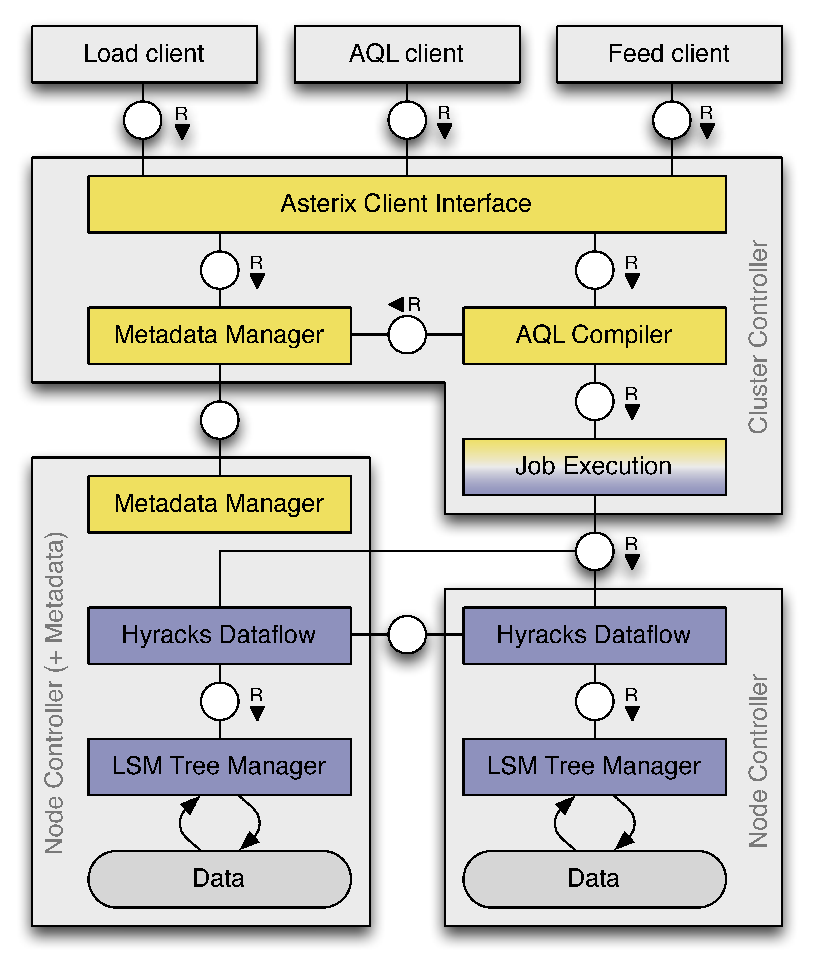
\includegraphics[width=2.7in]{images/asterixdb_arch}
%\vspace*{\betweenfigureandcaption}
\caption{Architecture\label{fig:arch}}
%\vspace{-0.1in}
\end{figure}

This node receives queries via an HTTP-based API and returns their results to the requester either synchronously or asynchronously (in which case a handle to the result is returned and the client can inquire about the query's status and request the result via the handle).
The Query Control Node also runs (a) the AQL compiler that translates AQL statements to Job Descriptions for the dataflow-engine Hyracks and (b) the Job Executor that distributes the Job Descriptions to the Hyracks Node Controllers and starts the execution. The AQL Compiler internally uses Algebricks to compile queries into Hyracks Jobs, that are then executed by the Hyracks Job Executor. Algebricks has access to the Metadata Manager through the metadata interface described in Section~\ref{subsec:metadata} in Chapter~\ref{ch:algebricks}.
The Worker Nodes -- represented by the boxes at the bottom of Figure \ref{fig:arch} -- have to (a) manage their partitions of the data stored in LSM-trees and to (b) run their parts of each Hyracks Job.
In the following subsection we will describe Hyracks and Algebricks. 

\begin{figure}[htb]
\centering
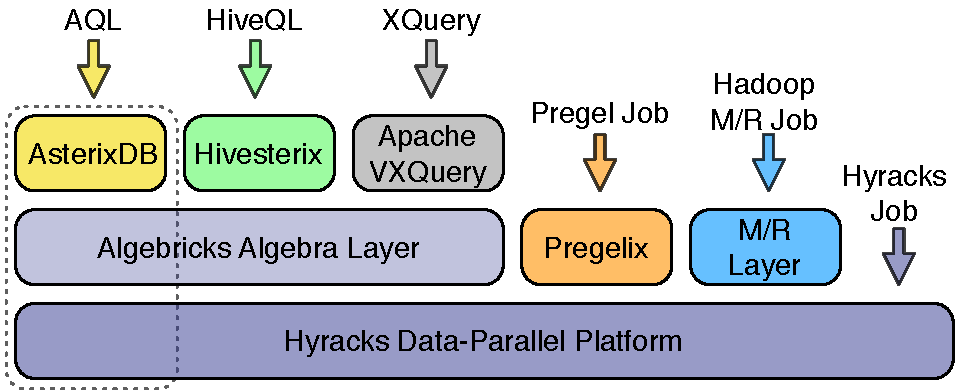
\includegraphics[width=5.0in]{images/asterixdb_stack}
%\vspace*{\betweenfigureandcaption}
\caption{Asterix software stack\label{fig:stack}}
%\vspace{-0.1in}
\end{figure}

\subsection{Hyracks and Algebricks}

The Hyracks layer of AsterixDB is the bottom-most layer of the Asterix software stack as described before, and shown in Figure \ref{fig:stack} repeated here for readability.
Hyracks is the runtime layer (\emph{a.k.a.}~executor) whose responsibility is to accept and manage data-parallel computations requested either by one of the layers above it in the Asterix software stack or potentially by direct end-users of Hyracks. 
In the case of AsterixDB, Hyracks serves as the scalable runtime engine for AQL queries once they have been compiled down into Hyracks Jobs for execution.

As mentioned before, jobs are submitted to Hyracks in the form of DAGs made up of \emph{Operators} and \emph{Connectors}. 
As described in \ref{ch:hyracks}, Hyracks Operators are responsible for consuming partitions of their inputs and producing output partitions. 
Connectors redistribute data from the output partitions and provide input partitions for the next Operator.

Figure \ref{fig:job} depicts the Hyracks Job for Query \ref{q:agg}.
The boxes represent its Operators and the lines represent Connectors.
One thing that we see is that all Connectors, except for the last one, are OneToOneConnectors. 
This means that no redistribution of data is required for this part of the plan---and it can be evaluated on the node that stores the data.
The degree of parallelism (the number of Operator instances evaluating in parallel) for these Operators is the number of partitions that is used to store the Dataset.
Looking at the Operators bottom-up, we see that the first 2 Operators perform a search on a secondary index.
This will return a set of primary key values that are fed into the search Operator on the primary index.
Note that the primary keys are sorted first to improve the access pattern on the primary index.
Above the primary index access we see two Operators that evaluate a predicate that should intuitively always be true for records that were identified by the search on the secondary index. This test is needed owing to the specific record-level transaction model implemented by AsterixDB. For more details about the transaction model supported by AsterixDB, please refer to~\cite{ASTERIX}.
Finally, we see that the \emph{avg} function that encapsulates the rest of the query has been split into two Operators: a \emph{Local Aggregation Operator} that pre-aggregates the records for the local node and a \emph{Global Aggregation Operator} that aggregates the results of the the Local Aggregation Operators.
Between these Operators is a MToNReplicatingConnector.
As the degree of parallelism for the Global Aggregation Operator is constrained to be 1, the Connector replicates the results of all instances of the Local Aggregation Operators to the single instance of the Global Aggregation Operator.
This split maximizes the distributed computation and minimizes network traffic.

\begin{figure}[htb]
\centering
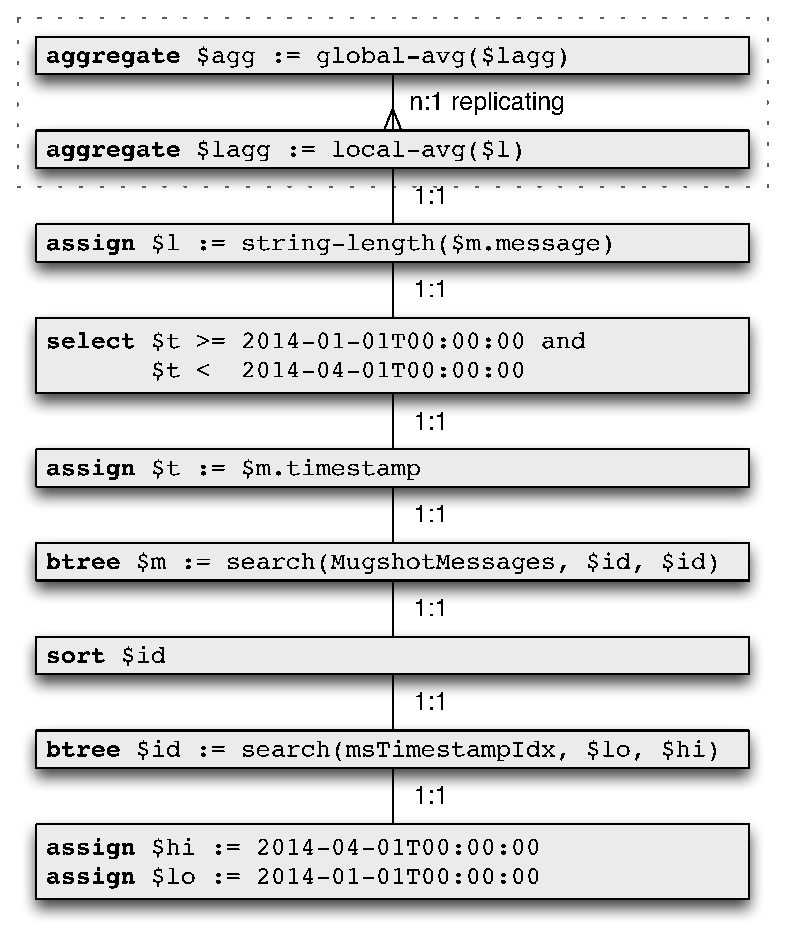
\includegraphics[width=3.0in]{images/hyracks-job2}
%\vspace*{\betweenfigureandcaption}
\caption{Hyracks job of the aggregation query in Query~\ref{q:agg}\label{fig:job}}
%\vspace{-0.1in}
\end{figure}

As the first step in the execution of a submitted Hyracks Job, its Operators are expanded into their constituent \emph{Activities}. 
While many Operators have a single Activity, some Operators consist of two or more Activities.
For example, a HybridHash Join Operator is made up of two Activities, the Join Build Activity and the Join Probe Activity. 
This expansion is made possible by APIs that Hyracks provides to Operator implementors to enable them to describe such behavioral aspects of an Operator.
Although Hyracks does not understand the specifics of the various activities of an Operator, exposing the blocking characteristics of Operators provides important scheduling information to Hyracks -- the separation of an Operator into two or more Activities surfaces the constraint that it can produce no output until all of its input has been consumed.

To execute a Job, Hyracks analyzes the Activity graph produced by the expansion described above to identify the collections of Activities (Stages) that can be executed at any time (while adhering to the blocking requirements of the Operators). 
Each Stage is parallelized and the resulting graph is executed in the order of the dependencies. 
More details about Hyracks' computational model, as well as its implementation and performance, are available in \cite{hyracks}.

The Hyracks job shown above, is generated by the Algebricks layer in AsterixDB. AsterixDB's AQL parser parses the query (Query~\ref{q:agg}, in this case) and produces a logical query expression using Algebricks operators, shown in the listing below.

\lstset{numbers=left, numberstyle=\tiny, stepnumber=1, numbersep=5pt}
\begin{center}
\scriptsize
\begin{lstlisting}
DISTRIBUTE-RESULT( $$temp1 )
PROJECT $$temp1
AGGREGATE $$temp1: avg( $$temp0 )
ASSIGN( $$temp0:string-length(
    field-access-by-name($$m, "message")) )
SELECT( algebricks-and(
    algebricks-ge(field-access-by-name($$m, "timestamp"), 
        datetime("2014-01-01T00:00:00")), 
    algebricks-lt(field-access-by-name($$1, "timestamp"), 
        datetime("2014-04-01T00:00:00")) )
UNNEST( $$m:dataset("MugshotMessages") ) 
EMPTY_TUPLE_SOURCE
\end{lstlisting}
\end{center}

After the initial logical plan is created, the compilation of the query proceeds using the Algebricks compiler. The metadata provider implemented within AsterixDB exposes source metadata to the Algebricks compiler. In the example above, the metadata provider is used to check if ``MugshotMessages'' is a valid dataset, and if so, also fetch the type associated with this dataset. In this specific instance, Algebricks realizes that the dataset has a secondary index on the ``timestamp'' field, and hence the time-range selection can be achieved by using that index. Based on this information, the Algebricks compiler rewrites the bottom part of the logical expression into one that would use the secondary index. Furthermore, Algebricks also optimizes the aggregate step of the query by converting it into a two-step distributed aggregate operation so that the amount of data transported over the network is minimized. The rewrite rule that utilizes indexes is specific to AsterixDB and lives in the AsterixDB codebase. On the other hand, the rule that optimizes aggregation for parallelism is available as part of the core Algebricks distribution.

AsterixDB uses the Algebricks framework to perform some optimizations specific to itself. As mentioned before, AsterixDB supports open types. A field accessed in a record of an open type might fall under one of two categories. The field could be one that was defined in the open type definition of the record type, or it could be a non-declared field. The concrete datamodel representation of record values in AsterixDB stores these two types of fields in different ways. Declared fields are stored without storing their field names in every record instance, and can be accessed using the index of the field. The undeclared fields, on the other hand, are stored along with their name. Although the declared fields can be accessed by name (by first probing the record type definition for the index, and then accessing the actual field value in the record instance by index), it is more efficient to ``constant-fold'' the name-to-index mapping step, so that the field can be looked up directly by index at runtime. AsterixDB uses a rewrite rule to perform data-flow analysis at compile-time to identify type lineage of values to maximize the locations in the query where the name-to-index mapping can be performed during compilation. All such occurrences of ``field-access-by-name'' invocations are then replaced by the ``field-access-by-index'' function, thus making the cost of accessing declared fields no worse than the costs associated with accessing fields in a fully typed language like SQL.

\section{Conclusion}

In this chapter, we took a look at AsterixDB, a semi-structured, parallel Big Data Management System and the roles of Hyracks and Algebricks in its architecture. Hyracks and Algebricks form core foundational pieces that provide significant functionality for compiling AQL queries and then running them in parallel on commodity clusters.

\chapter{Conclusions and Future Work}
\label{ch:conclusions-and-future-work}

This thesis presented Hyracks, a high-performance parallel dataflow runtime layer, and Algebricks, a parallel query compilation layer, both of which underpin the AsterixDB stack. Hyracks in conjunction with Algebricks also support quite a few other query processing systems. In addition to AsterixDB, described in Chapter~\ref{ch:asterixdb}, Hivesterix and Apache VXQuery are two other query processing engines that have been built on top of Hyracks + Algebricks. Hyracks has also served as a research platform for building specialized Big Data processing systems. Pregelix~\cite{pregelix} is a clone of the Pregel~\cite{Pregel} programming model for performing graph analytics over large distributed graphs, using a dataflow approach rather than a message-passing approach to solve the problem. Hyracks has also been used to implement a highly scalable version of the Batch Gradient Descent Algorithm for machine learning~\cite{DBLP:journals/corr/abs-1303-3517}.

Since Hyracks was first implemented and tested in 2011~\cite{hyracks}, we had the opportunity to test the software at scale (thanks to Yahoo! Research collegues who gave us access to their 180-node research cluster). The inter-process communication layers in Hyracks were re-architected based on lessons learned while running at that scale. Hyracks has also been used by outside groups as a research system. Researchers at Rice University used Hyracks to prototype Online Aggregation~\cite{DBLP:journals/pvldb/PansareBJC11}. A research group at UCSD working on Lineage Analysis instrumented Hyracks with their algorithms~\cite{Logothetis:2013:SLC:2523616.2523619}.

Hyracks still has a lot of room for improvement. For example, Hyracks implements a fairly simple form of fault-tolerance where a failed part of a job is re-executed until it succeeds. More sophisticated strategies, perhaps one that checkpoints operators periodically, could be used to reduce the amount of time spent in reruns. Furthermore, a cost-based analysis could be used to decide on the best operators to checkpoint in order to reduce the cost of the entire job. Automatic resource management is one other area that remains very open in the Hyracks platform. Distributing compute resources among concurrent queries is an important field of study that is not dealt with in this thesis. Hyracks uses a manual approach to resource management, where it is the programmer's or query compiler's responsibility to specify the amount of parallelism to use when running a job. In the future, Hyracks could benefit from an automatic resource management architecture, so that jobs could be optimized using various policies without the over (or under) consumption of available resources.

The Algebricks compilation framework has proven to be a valuable resource in building parallel query compilers, including several in addition to the AQL compiler in AsterixDB. As mentioned earlier, Algebricks has been used to build both Hivesterix (a Hive clone on Hyracks) and Apache VXQuery. Based on our experience building these query compilers, we have encountered some areas that could be explored in the future. Algebricks currently contains a rule-based optimizer. Cost-based optimization inside the Algebricks framework would be a welcome addition, and it would then benefit all the compilers built on top of Algebricks. In fact, the Database Research Group at IIT, Bombay has been working to embed their cost-based optimizer into the platform. Algebricks could also be extended to model iterative processing by perhaps adding an operator similar to the Alpha Operator~\cite{DBLP:journals/tse/Agrawal88}. Native iterative processing support would in turn allow Algebricks to be used to model systems like Pregelix and IMRU (both of which are currently hand-coded on top of Hyracks) and thus benefit from having an optimization step instead of relying on hand-coded plans as they do today.

AsterixDB, a project that originally started as a collaboration between the three Universities of California, at Irvine, Riverside, and San Diego, is now incubating at the Apache Software Foundation. Hyracks and Algebricks are now distributed as part of the AsterixDB project.


% These commands fix an odd problem in which the bibliography line
% of the Table of Contents shows the wrong page number.
\clearpage
\phantomsection

\bibliographystyle{abbrv}
\bibliography{bibliography,references}

\appendix

\end{document}
